\documentclass[12pt]{article}
\usepackage[utf8]{inputenc}
%\usepackage{nips_2017}
\usepackage{graphicx}
\usepackage{natbib}
\usepackage{booktabs}
\usepackage{float}
\usepackage{amsmath}
\usepackage{psfrag}
\usepackage{epsf}
\usepackage{enumerate}

%\bibliographystyle{apalike}

%\bibliographystyle{unsrt} % Use for unsorted references 
\newcommand{\blind}{0}

%\bibliographystyle{plainnat} % use this to have URLs listed in References

% DON'T change margins - should be 1 inch all around.
\addtolength{\oddsidemargin}{-.5in}%
\addtolength{\evensidemargin}{-.5in}%
\addtolength{\textwidth}{1in}%
\addtolength{\textheight}{1.3in}%
\addtolength{\topmargin}{-.8in}%

% Title Page

\bibliographystyle{natbib}

\def\spacingset#1{\renewcommand{\baselinestretch}%
{#1}\small\normalsize} \spacingset{1}

%%%%%%%%%%%%%%%%%%%%%%%%%%%%%%%%%%%%%%%%%%%%%%%%%%%%%%%%%%%%%%%%%%%%%%%%%%%%%%

\begin{document}

\if0\blind
{
  \title{\bf The Effect of Medicaid Expansion on Non-Elderly Adult Uninsurance Rates Among States that did not Expand Medicaid}
  \author{Max Rubinstein \hspace{.2cm}\\
    and \\
    Amelia Haviland \\ \\
    Heinz College and the Department of Statistics and Data Science \\ Carnegie Mellon University}
  \maketitle
} \fi

\if1\blind
{
  \bigskip
  \bigskip
  \bigskip
  \begin{center}
  \title{\bf The Effect of Medicaid Expansion on Non-Elderly Adult Uninsurance Rates Among States that did not Expand Medicaid}
\end{center}
  \medskip
} \fi

\bigskip

\begin{abstract}

We estimate the effect of Medicaid expansion on the adult uninsurance rates in states that did not expand Medicaid in 2014 using a novel extension of the synthetic controls approach (\cite{abadie2010synthetic}). The existing literature primarily estimates treatment effects on states that expanded Medicaid. We hypothesize these effects differ: evidence suggests that Medicaid take-up rates are lower among conservative states (\cite{sommers2012understanding}), and Republicans were more likely to govern non-expansion states. We therefore hypothesize that the treatment effect on states that did not expand Medicaid would have been closer to zero than for states that did expand Medicaid. Using data from the American Communities Survey (ACS), we estimate the effect on non-expansion states by re-weighting expansion regions to approximately balance the covariates from non-expansion regions. We contribute to the literature on balancing weights by accounting for hierarchical data and measurement error in the covariates when calculating our weights. We estimate that Medicaid expansion would have changed the uninsurance rate by -2.14 percentage points (-3.57, -0.71). These results are smaller in absolute magnitude than existing estimates of the ETT (see, eg, \cite{courtemanche2017early}). We provide evidence that factors associated with Republican governance may drive this difference.

\end{abstract}

\noindent%
{\it Keywords:} Balancing weights, synthetic controls, measurement error, regression calibration, treatment effect on the controls, Medicaid expansion, uninsurance rates
\vfill

\newpage
\spacingset{1.45} % DON'T change the spacing!

\maketitle

\section{Introduction}

The 2010 Affordable Care Act (ACA) required states to expand their Medicaid eligibility requirements by 2014 to offer coverage to all adults with incomes at or below 138 percent of the federal poverty level (FPL). The United States Supreme Court ruled this requirement unconstitutional in 2012, allowing states to decide whether to expand Medicaid coverage. In 2014, twenty-six states and the District of Columbia expanded their Medicaid programs. From 2015 through 2019 an additional ten states elected to expanded their Medicaid programs (\cite{KFF}). This first wave of expansions in 2014 enabled researchers to examine the effects of Medicaid expansion by using expansion states as ``treated'' states, and non-expansion states as ``control'' states. Our goal is to model the effect of 2014 Medicaid expansion on non-elderly adult uninsurance rates among states that did not expand Medicaid.

We predict that the treatment effect on non-expansion effect will be smaller in absolute magnitude than in states that expanded Medicaid in 2014. Medicaid take-up rates are lower than 100 percent and historically have varied across states. This variation is partly a function of state discretion in administering programs: for example, program outreach, citizenship verification policies, and application processes differ across states (\cite{courtemanche2017early}). Here we consider how political composition may have driven differences in take-up rates between states. Prior to the 2014 Medicaid expansion, \cite{sommers2012understanding} found that conservative political ideology was associated with lower Medicaid enrollment take-up rates, even after controlling for a variety of correlated policies. Most importantly, political ideology appears to have largely driven a state's decision to expand Medicaid in 2014. Figure~\ref{fig:stateideology} plots a measure of each state's 2013 institutional ideology by their Medicaid expansion status (\cite{fording}). Higher values of this score correspond to more liberal government institutions. The red dashed line indicates the mean expansion state score and the gray dashed line indicates the mean non-expansion state score. Figure~\ref{fig:stateideology} illustrates that non-expansion states are more conservative than expansion states.  If these differential take-up rates observed by \cite{sommers2012understanding} continue to hold post-expansion, we should expect treatment effects on non-expansion states to be smaller in absolute magnitude than treatment effects on expansion states. 

\begin{figure}
    \begin{center}
    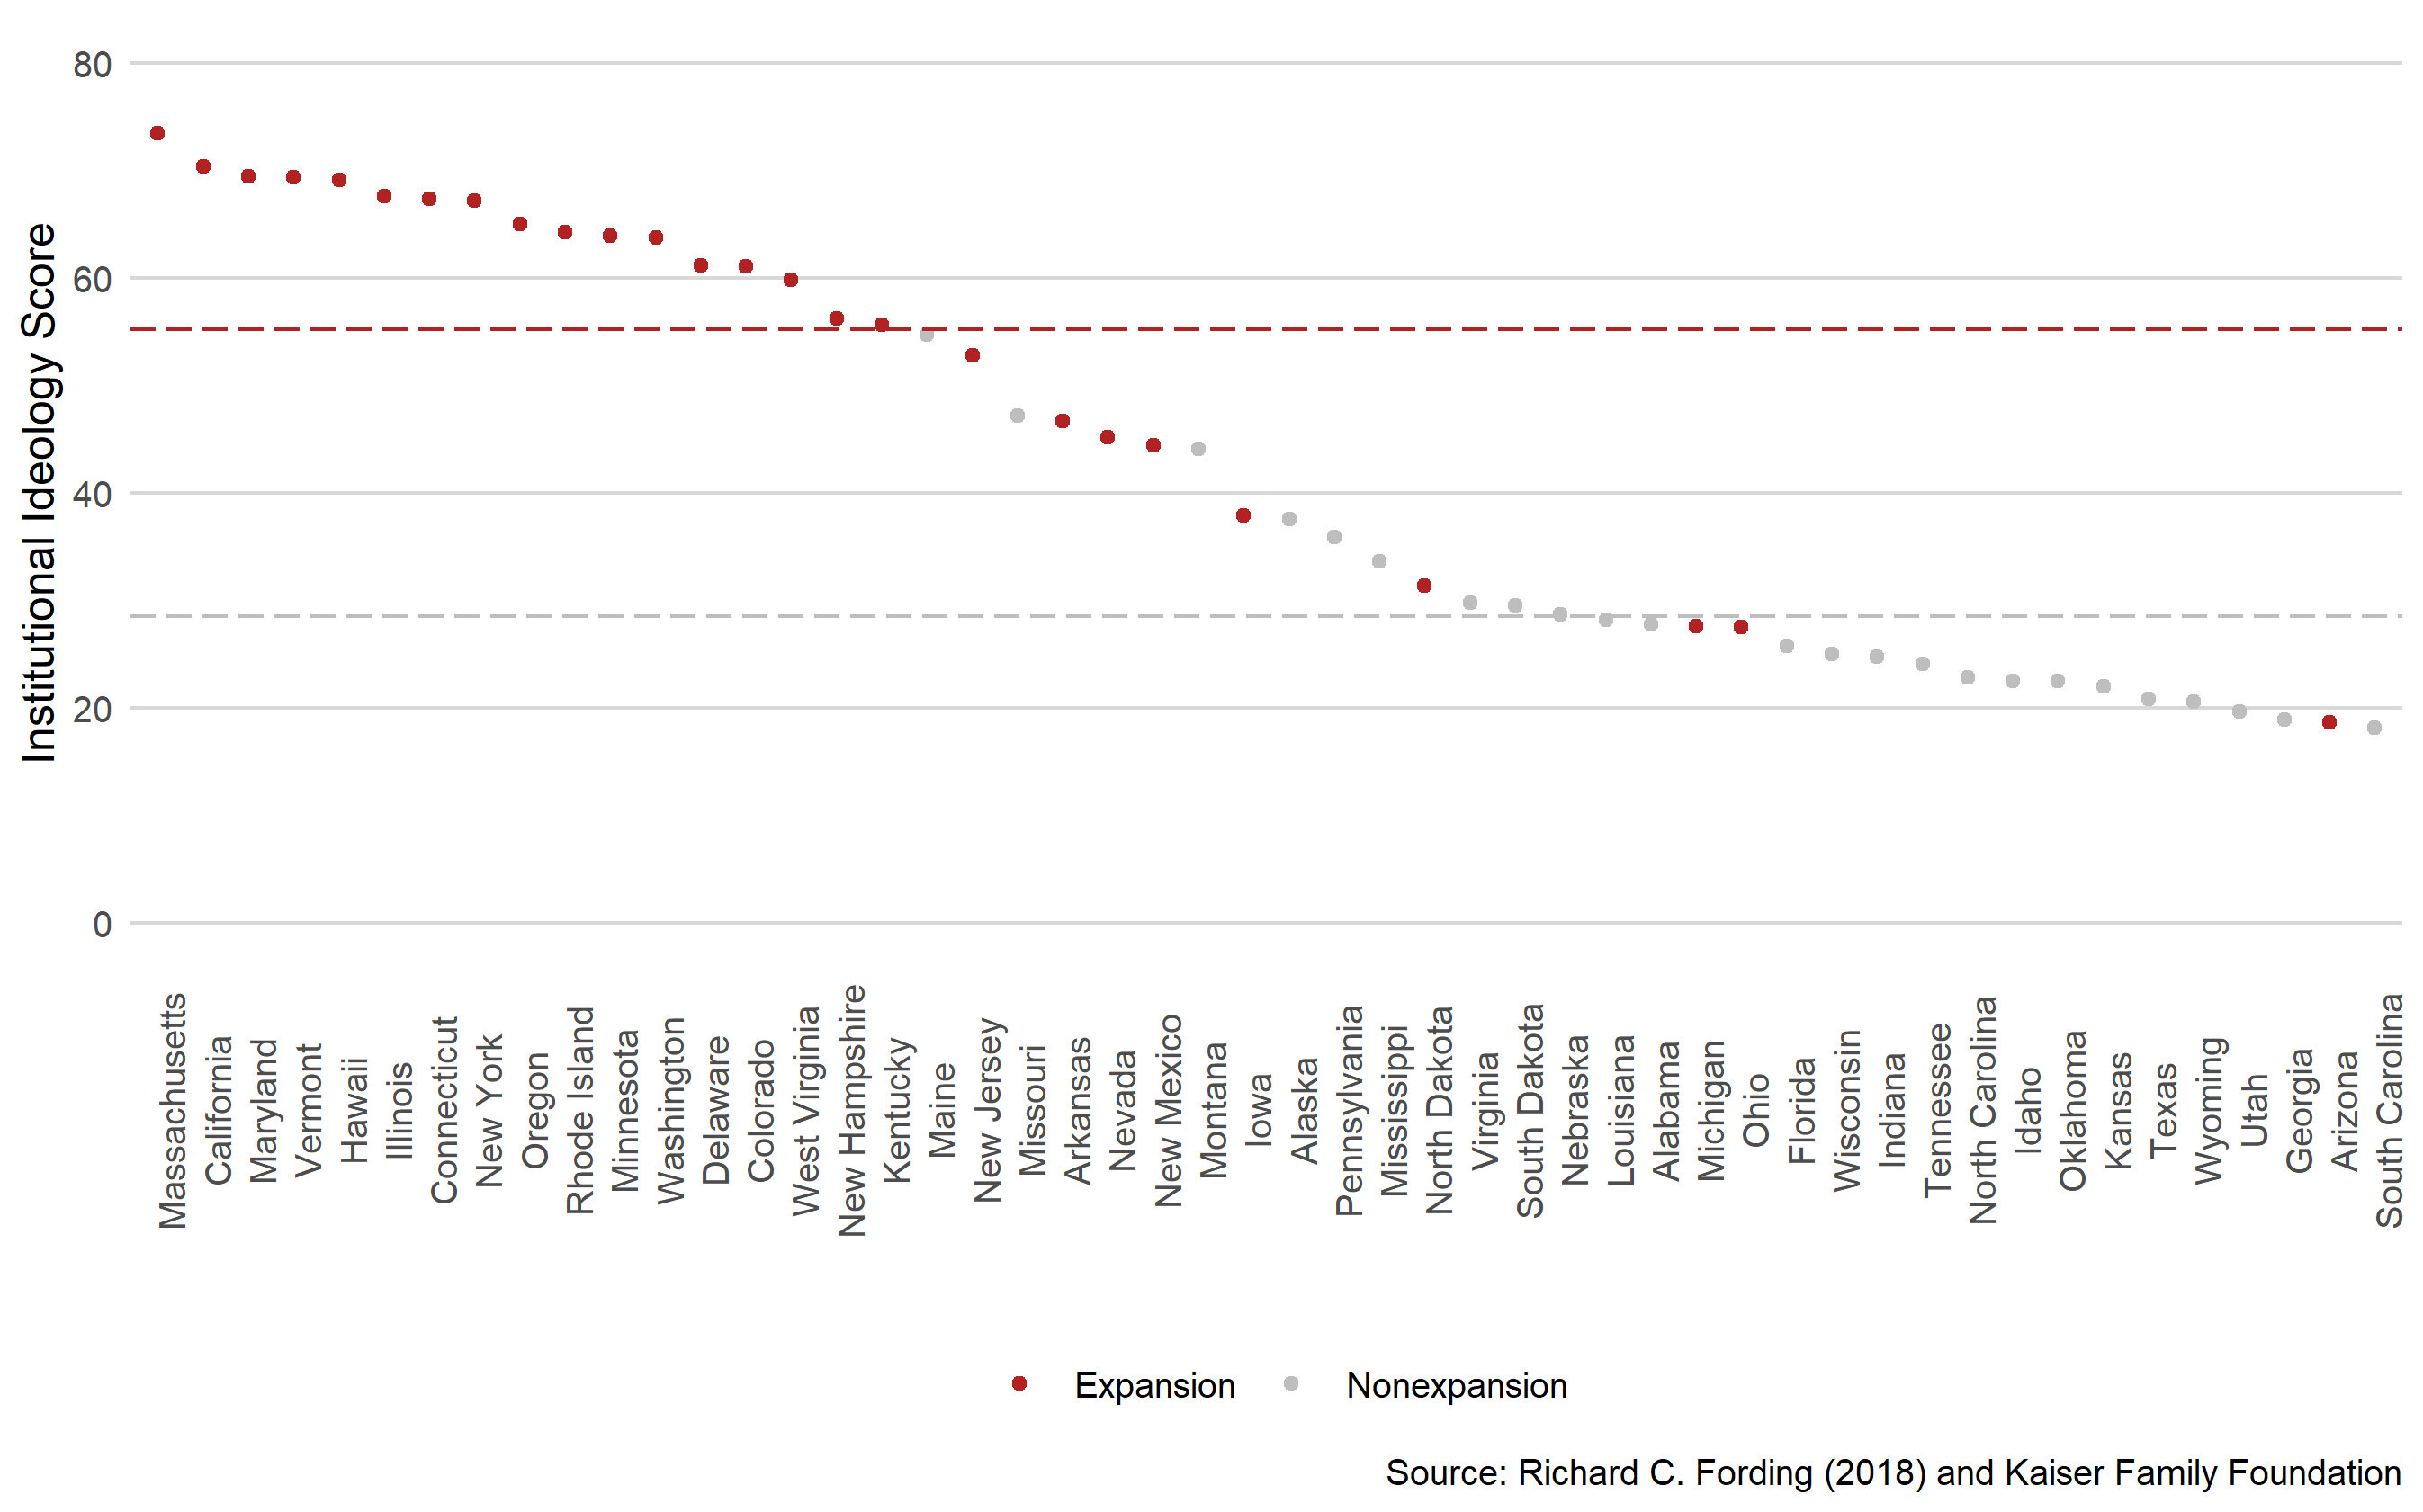
\includegraphics[scale=0.7]{01_Plots/political-expansion-plot.png}
    \caption{Government ideology and Medicaid expansion}
    \label{fig:stateideology}
    \end{center}
\end{figure}

This paper makes several methodological contributions. First, we extend the ``synthetic controls'' framework to estimate the treatment effect on the controls (ETC) and clarify the required assumptions. While balancing on pre-treatment outcomes alone arguably suffices for some synthetic control applications (see, eg, \cite{botosaru2017role}), here our goal is to estimate treatment response. We assume no unmeasured confounding given a rich covariate set and a linear and additive outcome model that accounts for all interactions between treatment and the covariates. Secondly, we use an implementation of Stable Balancing Weights (\cite{zubizarreta2015stable}) to estimate a set of positive weights to weight the expansion regions to approximately match the covariate distribution of the non-expansion regions. To account for remaining imbalances in the covariates, we also augment these weights with a regression-model following \cite{ben2018augmented}.

Our second contribution is to modify Stable Balancing Weights (SBW) for this setting. In particular, the SBW objective performs well assuming independent data with no measurement error. However, we use data from the American Communities Survey (ACS) aggregated to the consistent public use microdata area (CPUMA) level. These regions nest within states, and using these smaller regions allows us to get better balance on our covariates. However, as a result, our data both has a hierarchical structure (regions within states) and, because our region-level covariates are estimated from underlying survey data, the sampling variability used to estimate our covariates is a form of measurement error which may bias our treatment effect estimates. We propose a modification of the SBW objective function to account for the hierarchical nature of the data. We leverage the replicate survey weights provided in the ACS data to estimate the covariance matrix associated with the sampling variability and use this information to correct for this bias, following the regression calibration literature (see, eg, \cite{gleser1992importance}). This is the first study we are aware of that attempts to adjust for hierarchical data structure and measurement error in the covariates when using balancing weights. 

The remainder of this paper has the following structure. Section II provides an overview of the data and defines the study period, outcome, covariates, and treatment. Section III discusses our methods, beginning by defining our target estimand, and then outlining our identification, estimation, and inferential procedures. Section IV presents our primary results and sensitivity analyses. Section V provides a brief discussion of the policy relevance of our findings, and Section VI contains a brief concluding summary of the paper. Supplemental materials may be found in the Appendices.

\section{Data}

Our data source is the annual household and person public use microdata files from the American Community Survey (ACS) from 2011 through 2014. The ACS is an annual survey of approximately three million individuals across the United States. The public use microdata files include information on individuals in geographic areas greater than 65,000 people. The smallest geographic unit contained in these data are public-use microdata areas (PUMAs), arbitrary boundaries that nest within states but not within counties or other more commonly used geographic units. One limitation of these data is a 2012 change in the PUMA boundaries, which do not overlap well with the previous boundaries. As a result, the smallest possible geographic areas that nest both PUMA coding systems are known as consistent PUMAs (CPUMAs). The United States contain 1,075 total CPUMAs, with states ranging from having one CPUMA (South Dakota, Montana, and Idaho) to 123 CPUMAs (New York). The average total number of sampled individuals per CPUMA across the four years within our primary dataset of 929 CPUMAs (discussed in Section \ref{sssec:txassign}) is 1,001; the minimum number of people sampled was 334 and the maximum is 23,990.

\subsection{Study period}

We begin our analysis in 2011 following \cite{courtemanche2017early}, who note that several other aspects of the ACA were implemented in 2010 -- including the provision allowing for dependent coverage until age 26, and the elimination of co-payments for preventative care -- likely induced differential shocks across states. We also restrict our post-treatment period to 2014 only: several additional states expanded Medicaid in 2015, including Indiana, Michigan, and Pennsylvania. However, these states did not expand Medicaid contemporaneously with the 2014 ACA provisions. Without additional assumptions, this second-year expansion cannot help us estimate the effect of the 2014 expansion. 

\subsection{Covariates}

We use the underlying individual-level ACS survey data and accompanying survey weights to aggregate the data at the CPUMA level. We choose our covariates to approximately align with those considered in \cite{courtemanche2017early} and that are likely to be believe are potential confounders. Because we are ultimately interested in calculating rates, these variables include both the numerator and denominator counts.\footnote{We note that these ratio estimators will in general be biased; however, this bias decreases quickly with the sample size; given that our CPUMA sample sizes are all over 300 we treat these estimates as unbiased.}

Using the ACS survey weights, we first estimate: the total non-elderly adult population for each year 2011-2014; the total labor force population (among non-elderly adults) for each year 2011-2013; and the total number of households averaged from 2011-2013. We also construct an average of the total non-elderly adult population from 2011-2013. These are our denominator variables. For our numerator counts, we then estimate the total number of: females; whites; people born outside of the United States; citizens; people with less than high school education, high school degrees, some college, or college graduates or higher; people living under 138 percent of the FPL, between 139 and 299 percent, 300 and 499 percent, more than 500 percent, and who did not respond to the income survey question; total number aged 19-29, 30-39, 40-49, 50-64; households with one or more children, and who did not respond about children in their household. We average these estimated counts using the ACS survey weights from 2011-2013. For each individual year from 2011-2013, we also estimate the total number of people who were unemployed and uninsured at the time of the survey (calculated among all non-elderly adults and all non-elderly adult within the labor force, respectively). We divide the numerator counts by the corresponding denominator counts to estimate the percentage in each category. For the demographics, these include the average number of non-elderly adults from 2011-2013. For the time-varying variables, we use the corresponding year (where uninsurance rates are calculated as a fraction of the labor force rather than the non-elderly adult population). We also calculate the 2011-2012 and 2012-2013 population growth, and the average number of households to adult from 2011-2013. 

In addition to the ACS microdata, we use Census data to calculate the approximate percentage of people living within an ``urban'' area for each CPUMA (\cite{census}). Finally, we include three state-level covariates reflecting the partisan composition of each state's government in 2013. Specifically, we include an indicator for having a Republican governor, an indicator for Republican control over the lower legislative chamber, and an indicator for Republican control over both chambers of the legislature and the governorship.\footnote{Nebraska is the only state with a unicameral legislature; moreover, the legislature is technically non-partisan. We nevertheless classified them as having a Republican control of the legislature.} 

\subsection{Outcome}

Our primary outcome of interest is the non-elderly adult uninsurance rate in 2014, which we donate using $Y$. While take-up among the Medicaid-eligible population is a more natural outcome, we choose the non-elderly adult uninsurance rate for two reasons, one theoretic and one practical. First, Medicaid eligibility in the post-period is likely endogenous: Medicaid expansion may affect an individual's income and poverty levels, which in general define Medicaid eligibility. A second reason is to align our study to compare our results with the existing literature, and this is the outcome that \cite{courtemanche2017early} use. One implication of using this outcome is that the simultaneous adoption of other ACA provisions in 2014 more clearly affects this rate in a way that a more targeted group might not.

\subsection{Treatment assignment} \label{sssec:txassign}

While some states expanded Medicaid and other states did not, assigning a binary treatment status simplifies a more complex reality. There are three reasons to be cautious about this simplification. First, states differed substantially in prior Medicaid coverage policies: with perfect data we might consider Medicaid expansion as a continuous treatment with values proportional to the number of newly eligible individuals. The challenge though is correctly identifying newly eligible individuals in the data (see \cite{frean2017premium}, who attempt to address this). Second, \cite{frean2017premium} note that five states (California, Connecticut, Minnesota, New Jersey, and Washington) and the District of Columbia adopted partial limited Medicaid expansions prior to 2014. \cite{kaestner2017effects} and \cite{courtemanche2017early} also consider Arizona, Colorado, Hawaii, Illinois, Iowa, Maryland, and Oregon to have had early expansions. Lastly, timing is an issue: among the states that expanded Medicaid in 2014, Michigan's expansion did not go into effect until April 2014, while New Hampshire's expansion did not occur until September 2014.

Our primary analysis excludes New York, Vermont, Massachusetts, Delaware, and the District of Columbia from our pool of expansion states, because these states had comparable Medicaid coverage policies prior to 2014 (\cite{kaestner2017effects}). We also exclude New Hampshire because it did not expand Medicaid until September 2014. While Michigan expanded Medicaid in April 2014, we leave this state in our treated pool. We consider the remaining expansion states as ``treated'' and the non-expansion states as ``control'' states. We later consider the sensitivity of our results to these classifications by removing the early expansion states noted by \cite{frean2017premium}. Our primary classification of expansion and non-expansion states is unique among similar studies: \cite{courtemanche2017early} classifies all expansion states as treated, and all non-expansion states as control. \cite{frean2017premium} exclude Massachusetts from expansion states. Lastly, \cite{kaestner2017effects} include Delaware, the District of Columbia, Massachusetts, New York, and Vermont as control states. Our final dataset contains aggregated statistics for all of the above variables for 925 CPUMAs in our non-expansion and our pool of expansion states. 414 CPUMAs among 24 non-expansion states and 515 CPUMAs among 22 expansion states. When we exclude the early expansion states, we are left with 296 CPUMAs across 17 states.

\section{Methods}
\label{sec:methods}

In this section we present our causal estimand, identifying assumptions, estimation strategy, and inferential procedure. Additional details are available in the Appendix.

\subsection{Estimand}

We seek to estimate the average effect 2014 Medicaid expansion would have had on the non-elderly adult uninsurance rate in states that did not expand Medicaid. The 2014 Medicaid expansion occurred simultaneously with the implementation of several other major ACA provisions, including (but not limited to) the creation of the ACA-marketplace exchanges, the individual mandate, health insurance subsidies, and community-rating and guaranteed issue of insurance plans (\cite{courtemanche2017early}). Almost all states broadly implemented these reforms beginning January 2014. Conceptually we think of the other ACA components as a state-level treatment ($V$) separate from Medicaid expansion ($A$).

Let $c$ index a CPUMA, $s$ index the state, and $t$ index the time period. Let $N_1$ be the number of treated CPUMAs, $N_0$ be the number of control CPUMAs, and $N$ be the total number of CPUMAs. Similarly, let and $M = M_0 + M_1$ states (with $M_0$ and $M_1$ defined analogously). Each state has $n_s$ CPUMAs. Finally, let $Y_{scT}^{A_{scT} = a, V_{scT} = v}$ be the potential uninsurance rate given Medicaid expansion and other ACA-reforms at time $T = 2014$. We wish to estimate the following contrast:

$$
\psi &= \psi^1 - \psi^0 \\
&=N_0^{-1}\sum_{s: A_{sT} = 0, V_{sT} = 1}^{M_0}\sum_{c = 1}^{n_s} Y_{scT}^{A_{scT} = 1, V_{scT} = 1} - Y_{scT}^{A_{scT} = 0, V_{scT} = 1} 
$$

In other words, we want to estimate the difference in the non-elderly adult uninsurance rates among states that did not expand Medicaid, but did implement other aspects of the ACA. Because all states implemented the ACA marketplace expansion in 2014, contrasts with the corresponding potential outcome absent this expansion are not identified. Moreover, since we are only interested in the counterfactual at time $T$, we simplify notation by removing this variable and the subscript in the estimand:

$$
\psi = N_0^{-1}\sum_{sc: A_s = 0} Y_{sc}^{A_{sc} = 1} - Y_{sc}^{A_{sc} = 0}
$$

We therefore seek to identify the effect of Medicaid expansion in the context of the simultaneous implementation of the ACA, but do not attempt to separately identify the effects of these separate treatments. Because interactions between the ACA implementation and Medicaid expansion may vary over time, we do not seek to generalize these results outside of 2014. 

\subsection{Identification}

We make the following causal assumptions: consistency, no unmeasured confounding, no anticipatory treatment effects, and positivity of treatment assignment. We explain these assumptions in detail and why we think they might be reasonable in this context. We additionally make several parametric assumptions to help us identify our parameter given the problem of measurement error in our covariates.

Consistency states that the observed factual outcome under a given treatment assignment is equal to the potential outcome under that same treatment assignment ($Y_{sc}^{A_{sc} = a} = Y_{sc} \mid A_{sc} = a$). In other words, we assume that one regions' treatment assignment didn't affect another regions' observed outcome. This is a standard assumption, but is often not realistic. Violations of this assumption are likely in our setting: for example, \cite{frean2017premium} find evidence that Medicaid expansion drove previously eligible but uninsured individuals to enroll in Medicaid in both expansion and non-expansion states. Signing the potential bias from these spillovers requires redefining the causal estimand: for example, we might consider the treatment effect on the untreated given that all states have expanded Medicaid, where the contrast is against where only the observed expansion states expanded Medicaid. If spillovers occurred in equal proportions in each region, and the magnitude of the spillovers increase with the number of treated regions, then the true effect would be larger in absolute magnitude than the estimated estimated using the observed data. We could consider other estimands or assumptions to get different predictions about the sign of the bias, but we leave this as an area for future work.

We next assume that there were no anticipatory treatment effects. Letting treatment occur at time $T$, we have that for $t < T$:

$$
Y_{sct} = Y_{sct}^0
$$

This assumption is necessary because we are conditioning on pre-treatment outcomes. If these outcomes were affected by the treatment before it were implemented, these covariates would not be exogenous. Anticipatory treatment effects may occur if plans to expand Medicaid induce uninsured but Medicaid-eligible individuals to enroll in Medicaid prior to expansion. We do not think these violations occurred in large enough numbers to substantially affect our results. Instead, we address a more concerning version of this violation: as noted above, several states allowed certain counties to expand Medicaid prior to 2014. We therefore test the sensitivity of our results to the inclusion of these states.

Third, we assume no unmeasured confounding; that is, that at time $T$ the potential outcomes for each CPUMA are independent of the state-level treatment assignment conditional on the population-level CPUMA and state-level covariates $X_{sc}$ (which includes pre-treatment outcomes):

$$
Y_{sc}^a \perp A_{sc} \mid X_{sc}
$$

While unverifiable, we believe it is reasonable here given our rich covariate set. To be explicit, we believe that the potential uninsurance rates for each CPUMA given treatment is independent of the CPUMA's treatment assignment conditional on the percentage of uninsured individuals in each year of the pre-treatment period, the percentage of unemployed individuals in each year of the pre-treatment period, the population growth in 2012 and 2013, the average ratio of households to non-elderly adult population, the state's political composition, the average proportion of households with one or more children during the pre-treatment period, the average number of households who did not respond about their number children, and the average proportion of individuals during the pre-treatment period with given demographics noted above (age, sex, white, Hispanic ethnicity, US citizenship, foreign born, income-to-poverty group (including non-response), disability status, urban residence, and educational attainment group). If this assumption were violated -- that is, other covariates exist that determine this potential outcome and treatment assignment -- conditioning on pre-treatment outcomes is likely to help proxy for these covariates, thereby minimizing the potential for bias. 

Unfortunately we do not actually observe the true values of $X_{sc}$ but rather an estimate $W_{sc}$. Importantly, $Y_{sc}^a \perp A_{sc} \mid X_{sc} \not\implies Y_{sc}^a \perp A_{sc} \mid W_{sc}$. Therefore, the use of these proxies may also bias our estimates. We rely on several modeling assumptions outlined below in our estimation procedure to correct for this bias.

Finally, we assume positivity of treatment assignment; that is, that all states had some probability of being treated $\pi(X_{1s}, ..., X_{n_ss}) > 0$. Positivity violations can cause a lack of covariate overlap in the observed data. As we have noted before, overlap is an issue in this study. We address this in multiple ways that we outline in our estimation strategy below. 

These assumptions are sufficient to non-parametrically identify our causal estimand if we observed the true covariates $X_{sc}$. We next invoke parametric modeling assumptions that help us identify our estimand given that we observe the mean unbiased sample estimates $W_{sc}$. First, we assume that the potential outcome under treatment is linear and additive in the covariates $X_{sc}$. Specifically, we assume that the following model generates the potential non-elderly adult uninsurance rate under treatment:

$$
Y_{sc}^1 = \alpha + X_{sc}^T\beta + \epsilon_{sc} + c_s
$$

We assume that the errors $\epsilon_{sc}$ and $c_s$ are independent from each other and across time (ie we rule out serial-correlation), and that these errors are invariant to the intervention. This model then allows us to identify $\psi^1$ in terms of our model parameters; specifically, we have that $\psi^1 = \alpha + \bar{X}_0^T\beta$, where $\bar{X}_0$ is the (observed) mean covariate values among the control units.\footnote{To be precise, we use the population-weighted mean so as to target the individual-level treatment effect rather than the CPUMA-average treatment effect.} Let $s_{sc}$ be the vector of sample sizes used to calculate $W_{sc}$. We then assume that that $W_{sc} = X_{sc} + v_{sc}$, where $\sqrt{s_{sc}}v_{sc}$ are drawn independently from $MVN(0, \Sigma_{vv})$, and $v_{sc}$ is independent of the CPUMA-level errors $\epsilon_{sc}$ (which may include measurement error in the outcome) and the state-level errors $c_s$. We do not believe the errors in the CPUMA-level aggregates are correlated with the CPUMA outcome errors because the outcomes are estimated from a different cross-section of individuals than the covariates; therefore, any estimation error in $Y_{sc}$ is likely independent of $v_{sc}$. Moreover, because the measurement error comes from sampling variability, assuming that the error is normally distributed is reasonable.\footnote{While the sample sizes for each CPUMA are all relatively large, the variance is still larger than one might expect due to the design effect of the survey.} Using results from the measurement error literature, these parameters, and therefore our causal estimand, are identified if we know $\Sigma_{vv}$ (see, eg, \cite{gleser1992importance}). We discuss this further in Appendix A, while connecting these results to weighting estimators that directly estimate $\psi^1$ rather than outcome models that estimate $(\alpha, \beta)$. 

\subsection{Estimation}

We outline our estimation strategy first emphasizing how our method differs from the synthetic controls approach. In particular, we explain why estimating the ETC must rely on arguably stronger assumptions than the ETT. We then explain these how these assumptions differ from synthetic control applications and why we therefore choose to use an implementation of Stable Balancing Weights (SBW) for our modeling. Second, we explain a modification we make to the SBW criterion (which we call H-SBW) to address the hierarchical data structure and show that it reduces the variance of our estimator under our assumption of within-state correlation of our model errors. Third, we connect our estimator to the regression calibration literature by generating weights that balance on an imputation of the true covariates $\hat{\eta}(W_{sc})$. Finally, due to remaining imbalances in our covariates, we debias our estimator using ridge-augmented weights, following the suggestion of \cite{ben2018augmented}. As a sensitivity check, we also use overlap weights, to estimate a different causal parameter -- the overlap average treatment effect (OATE) -- as suggested by \cite{li2018balancing}.

Similar to synthetic controls applications, we seek to generate a set of positive weights that balance the means of covariates for the treated units to the mean of covariates for the control units. Assume that we observe the true covariates $X_1$ and $X_0$, and let $\bar{X}_0$ be the (population-weighted) average of the covariate values in the non-expansion region. Ideally, we could then find some $\gamma^\star$ such that for $\delta = 0$: 

$$
((N_0^{-1})X_1^T\gamma^\star - \bar{X}_0) \le \delta, \gamma_i^\star > 0, \sum_{sc} \gamma_{sc}^\star = N_0
$$

Let $p$ be a vector of (normalized) population weights for each CPUMA in the non-expansion region in year $T = 2014$. We could then estimate $\psi$ as

$$
\hat{\psi} = (N_0^{-1}\sum_{s: A_s = 1}^{M_1}\sum_{c = 1}^{n_s}\gamma_{sc}^\star Y_{sc} - \sum_{s: A_s = 0}\sum_{c = 1}^{n_s}Y_{sc}p_{sc})
$$

While synthetic controls are frequently motivated by the assumption that the outcomes follow a linear factor model, here we assume no unobserved confounding and that $\mu_1(X_{sc}) = \alpha + X_{sc}^T\beta$. The bias of our estimator is therefore less than or equal to $\beta^T \delta = 0$ (see, eg, \cite{zubizarreta2015stable}). The challenge, however, is that for any given dataset we have no guarantee that any such $\gamma$ exists that exactly balances the covariates; we therefore need some method of determining how to prioritize which parts of the covariate distribution we wish to balance to control the bias.

This is where our method to estimate the ETC contrasts with the commonly used synthetic control approach used to estimate the ETT: \cite{abadie2010synthetic} determine how to prioritize covariate balance by training their model on pre-treatment outcomes (\cite{kaul2015synthetic} shows that often the most relevant covariates simply become the pre-treatment outcomes). Because in that setting $Y^0_{sct}$ is actually observed for $t \le T_0$, \cite{abadie2010synthetic} leverage this data to select the covariates that best predict these values. By contrast we never observe $Y^1_{sct}$ prior to treatment. Without additional assumptions, we cannot use the pre-treatment data to learn which covariates matter most for determining this potential outcome.

Moreover, the problem of predicting treatment response also makes estimating the ETC more challenging than the ETT. As a result, we may care far more about balancing ``auxillary covariates'' (ie covariates that are not pre-treatment outcomes) in our setting than the traditional synthetic controls setting. Consider the following example: say for some application there exist two sets of weights, $\gamma_1$ and $\gamma_2$, that exactly balances $k$ pre-treatment means of the controls units to the treated unit(s). $\gamma_1$ additionally exactly balances $p$ auxillary covariates, while $\gamma_2$ does not. Heuristically, estimates using either set of weights may provide reasonable estimates of the counterfactuals for the treated unit(s) absent treatment. However, now consider inverting the treatment assignment -- ie the control units are treated and the treated units control -- and predicting the outcome under treatment for those not treated: intuitively, we should choose $\gamma_2$. Why? Because we might worry that these observable characteristics predict not just outcome levels without treatment but also treatment response, and the treatment response of these two units might differ substantially. 

More formally, assume that $\mu_0(X_{sc})$ is linear in the covariates. We might reasonably believe the coefficients on auxillary covariates are close to zero once we condition on pre-treatment outcomes. As a result, the bias induced by imbalances on these covariates would be small. On the other hand, the coefficients on the same covariates for the model $\mu_1(X_{sc})$ could be much larger, even after conditioning on pre-treatment outcomes. If our synthetic control weights fail to balance these covariates, we should expect that our estimates of $\mu_0$ will in general have less bias than our estimates of $\mu_1$. In summary, estimating the ETC requires a greater understanding of how the covariates are related to treatment response than the ETT; moreover, and we cannot learn this information by using pre-treatment outcomes.

We therefore estimate the ETC by using a variation of SBW that we call H-SBW.\footnote{Specifically, we use a modified implementation of Noah Griefer's ``optweight'' package in R, available on github.com/mrubinst757}. This procedure allows us to estimate the minimum variance weights that satisfy certain balance constraints. Let $\eta_a(W_{sc}) = \mathbb{E}\{X_{sc} \mid W_{sc}, A_s = a\}$, and $\hat{\eta}_1(W_1)$ be a matrix of estimates of $\eta(W_1)$. Let $\bar{W}_0$ be a vector of population-weighted estimates of the covariates for the non-expansion region.\footnote{Because $\bar{W}_0$ is in expectation equal to $\bar{X}_0$, the use of this target will not bias our estimator.} We generate weights that solve the following objective:

$$
\min_{\gamma \in \Gamma} \sum_{s: A_s = 1}^{M_1}(\sum_{c = 1}^{n_s} \gamma_{sc}^2 + \sum_{c \ne d}\rho \gamma_{sc}\gamma_{sd})
$$

$$
\Gamma := \{\gamma \mid N_0^{-1}\hat{\eta}_1(W_{sc})^T\gamma - \bar{W}_0 \mid \le \delta, \gamma_{sc} > 0, \sum_{sc}\gamma_{sc} = N_0\}
$$

Unlike the synthetic controls objective, the SBW objective allows the user to specify covariate-level balance constraints using the vector $\delta$. When estimating the ETC, we lean heavily on assumptions to justify our choice of $\delta$; in particular, we use a priori domain knowledge about which covariates are most likely to be important predictors of treatment effect heterogeneity when setting $\delta$. 

We now discuss how the H-SBW criterion differs from SBW. Notice that the SBW criterion is equivalent to ours when setting $\rho = 0$; in other words, SBW attempts to calculate the minimum variance weights for a fixed $\delta$. This is desirable if, for example, the errors in the outcome model are all independent and identically distributed. In our case, we account for possible state-level dependencies in the outcome model. Intuitively, by adding the tuning parameter $\rho$, this objective attempts to ensure that the within state sum of weights is roughly uniform across states as well as across CPUMAs. This is especially desirable if many weights would in some cases be concentrated in only one state. We discuss this objective in more detail and provide simulation results in Rubinstein et al (2021) (not yet available); broadly speaking, we can think of H-SBW being to SBW what generalized least squares (GLS) is to ordinary least squares (OLS): both SBW and OLS can produce unbiased estimates of certain parameters, but H-SBW and GLS are more efficient estimators assuming a block-matrix correlation structure in the outcome errors.

A second departure from SBW comes in the constraint set: rather than balancing on the observed covariate values $W_{sc}$, we instead balance on our estimate of $\eta_1(W_{sc})$. This is because the estimation error in these CPUMA-level covariates will bias our estimate of $\psi^1$. In Appendix A we show that this bias is equivalent to the bias induced in the classical measurement error framework using OLS. We further show that if we had access to $\eta_1$, we could get an unbiased estimate of $\psi^1$. Here we leverage the person-level replicate survey weights provided in the ACS microdata to estimate the variability in each CPUMA's observed covariate values. We then use a variant of regression calibration techniques to estimate $\eta_a(W_{sc})$ as a linear approximation to the true covariate values (see, eg, \cite{gleser1992importance}, \cite{carroll2006measurement}). We consider two versions of this procedure: our preferred version which accounts for the fact that some covariate values are estimated much more precisely than other values; and a second that follows the traditionally used procedures in this setting which does not account for this differential precision. Further details about these covariate adjustment procedures in Appendix B.

This is the first application we are aware of to use regression calibration methods in the context of balancing weights. We emphasize the key assumptions for the theoretical groundings for this procedure: (1) the outcome model is linear in the covariates; (2) the measurement error in the outcome is unrelated to the measurement error in the covariates; (3) the covariates are randomly sampled from some larger super-population. The first assumption is quite strong, though standard in many applications. The second assumption is reasonable, because our outcomes are estimated from a different cross-section of individuals than our covariates. The final assumption is not strictly necessary, though is often invoked to motivate using regression-calibration methods (see, eg, \cite{gleser1992importance}). 

Lastly, we are unable to achieve exact balance. These imbalances may well bias our estimator. Following the recent literature on synthetic controls, we reduce this bias by using ridge-regression augmented weights \cite{ben2018augmented}. Letting $\hat{\eta}_1(W_1)$ be the matrix of adjusted covariates, we standardize our weights to sum to one and use the regression-augmented weights:

$$
\gamma^{aug} = \gamma^{sbw} + (\hat{\eta}_1(W_1)^T\gamma^{sbw} - \bar{W}_0)^T(\hat{\eta}_1(W_1)^T\Omega^{-1}\hat{\eta}_1(W_1) + \lambda I_d)^{-1}\hat{\eta}_1(W_1)^T\Omega^{-1}
$$

where $\Omega$ is a block diagonal matrix with diagonal entries equal to one and the within-group off diagonals equal to $\rho$. We choose $\lambda$ so that the remaining imbalances all fall within 0.1 percentage points (see \cite{ben2018augmented} for more details on the connection between these weights and ridge-regression). The cost of this de-biasing procedure is that we must extrapolate from the support of the data, and therefore rely more heavily on our modeling assumptions. Finally, notice that we can also generate Oaxaca-Blinder weights ($\gamma^{ob}$) by setting $\gamma^{sbw} = 1/N_0$ and $\lambda = 0$. These are equivalent to running OLS (or GLS) on the observed outcomes among the treated units and imputing the missing counterfactual using these coefficient estimates. In our results we consider estimators using SBW ($\rho = 0$), $H-SBW$ ($\rho = 0.2$), and ridge-augmented versions of SBW and H-SBW that we call BC-SBW and HC-HSBW. We also generate Oaxaca-Blinder weights setting $\rho \in \{0, 0.2\}$ (OB and H-OB) and provide these results in Appendix D. We focus our discussion on our preferred estimators, H-SBW and the ridge augmented version BC-HSBW. 

\subsection{Inference}

We treat our estimate of $\psi^0$ as known, since the population-weighted CPUMA average of observed values is quite precisely estimated relative to the CPUMA-level averages. We then evaluate the uncertainty in our estimator with respect to our model-based estimates of $\psi^1$ and $\eta_1(W_{sc})$. We use the leave-one-state-out jackknife to estimate the standard error of our estimator of $\psi^1$ (\cite{cameron2015practitioner}). We compute standard errors both recalculating all of the estimators on the adjusted dataset using our estimates of $\eta_1(W_{sc})$, and also recalculating the estimators including the entire adjustment process. We expect that either of these estimators will be conservative: our target of inference is a finite-sample estimand while the bootstrapped standard errors give asymptotic coverage for imagined super-population effects (see, eg, \cite{imbens2015causal}). Moreover, it is not clear that resampling entire states to approximate the variability from our estimate of $\eta_1(W_{sc})$ is a sensible procedure when we view the underlying covariates as fixed, since, conditional on $X_{sc}$, it is reasonable to assume that the sampling variability is drawn independently at the CPUMA rather than the state-level. We therefore present the standard errors that are conditioned on the adjustment process in the paper, and leave the full-procedure jackknife confidence interval results to Appendix D. 

\section{Results}

We present the following results using our preferred covariate adjustment $\hat{\eta}_1(W_{sc})$.  Figure~\ref{fig:loveplot} shows how our balancing weights reduce the imbalances among covariates with greater than one percentage point difference between the targeted mean in the expansion region and the mean values in the non-expansion region (we target the population-weighted mean of the untreated region). Before applying our weights, we see that there are substantial imbalances in the republican governance indicators, as well as pre-treatment uninsurance and unemployment rates. Our weights drastically reduce these differences; however, some imbalances remain. In particular, imbalances remain in the Republican governance indicators. A full balance table is available in Appendix C. 

\begin{figure}[B]
\begin{center}
    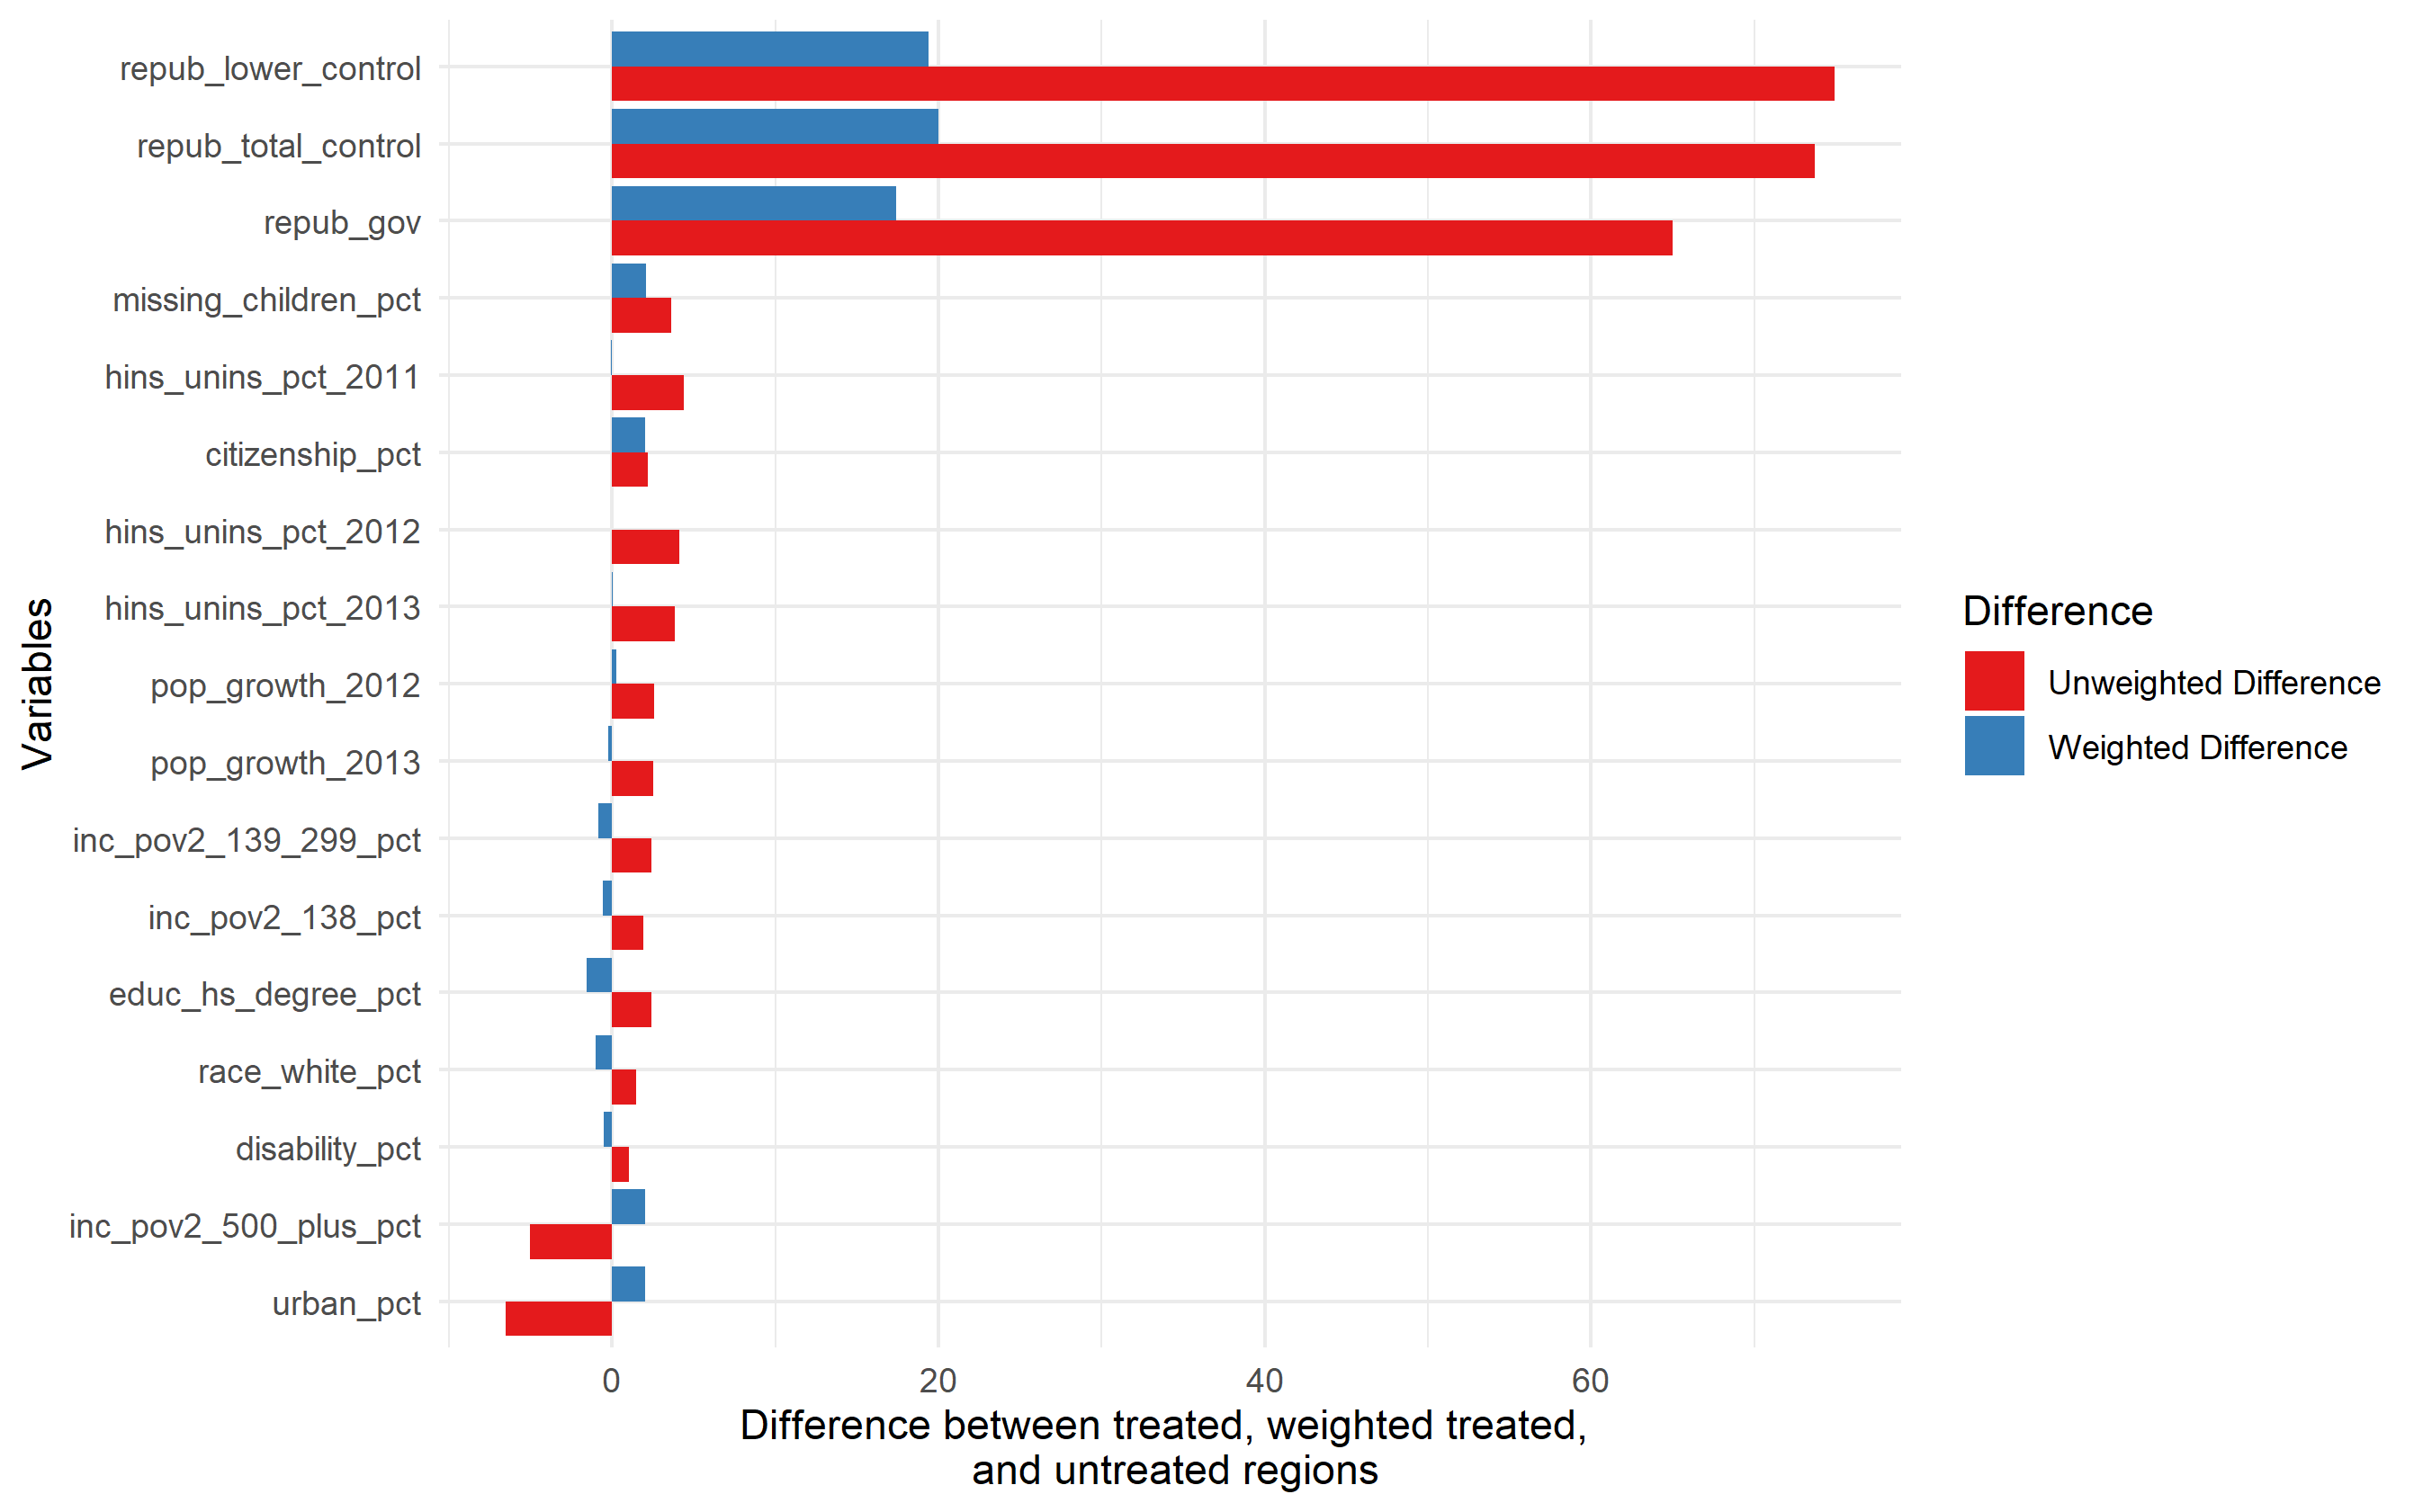
\includegraphics[scale=0.6]{01_Plots/balance-plot-etu.png}
    \caption{Balance plot}
    \label{fig:loveplot}
\end{center}
\end{figure}

As discussed above, we then use ridge-regression augmentation to extrapolate from the data in order to reduce all imbalances within 0.1 percentage points. Figure~\ref{fig:statewghts} shows the total weights summed across states for each estimator: H-SBW and BC-HSBW. This figure sums the negative weights separately from the positive weights to make clear the extent of the extrapolation. We see that BC-HSBW extrapolates heavily in order to estimate the counterfactual, particularly for CPUMAS in California. Due to this extensive extrapolation, we therefore prefer the H-SBW estimator, though we compare results against BC-HSBW as a robustness check.

\begin{figure}[B]
\begin{center}
    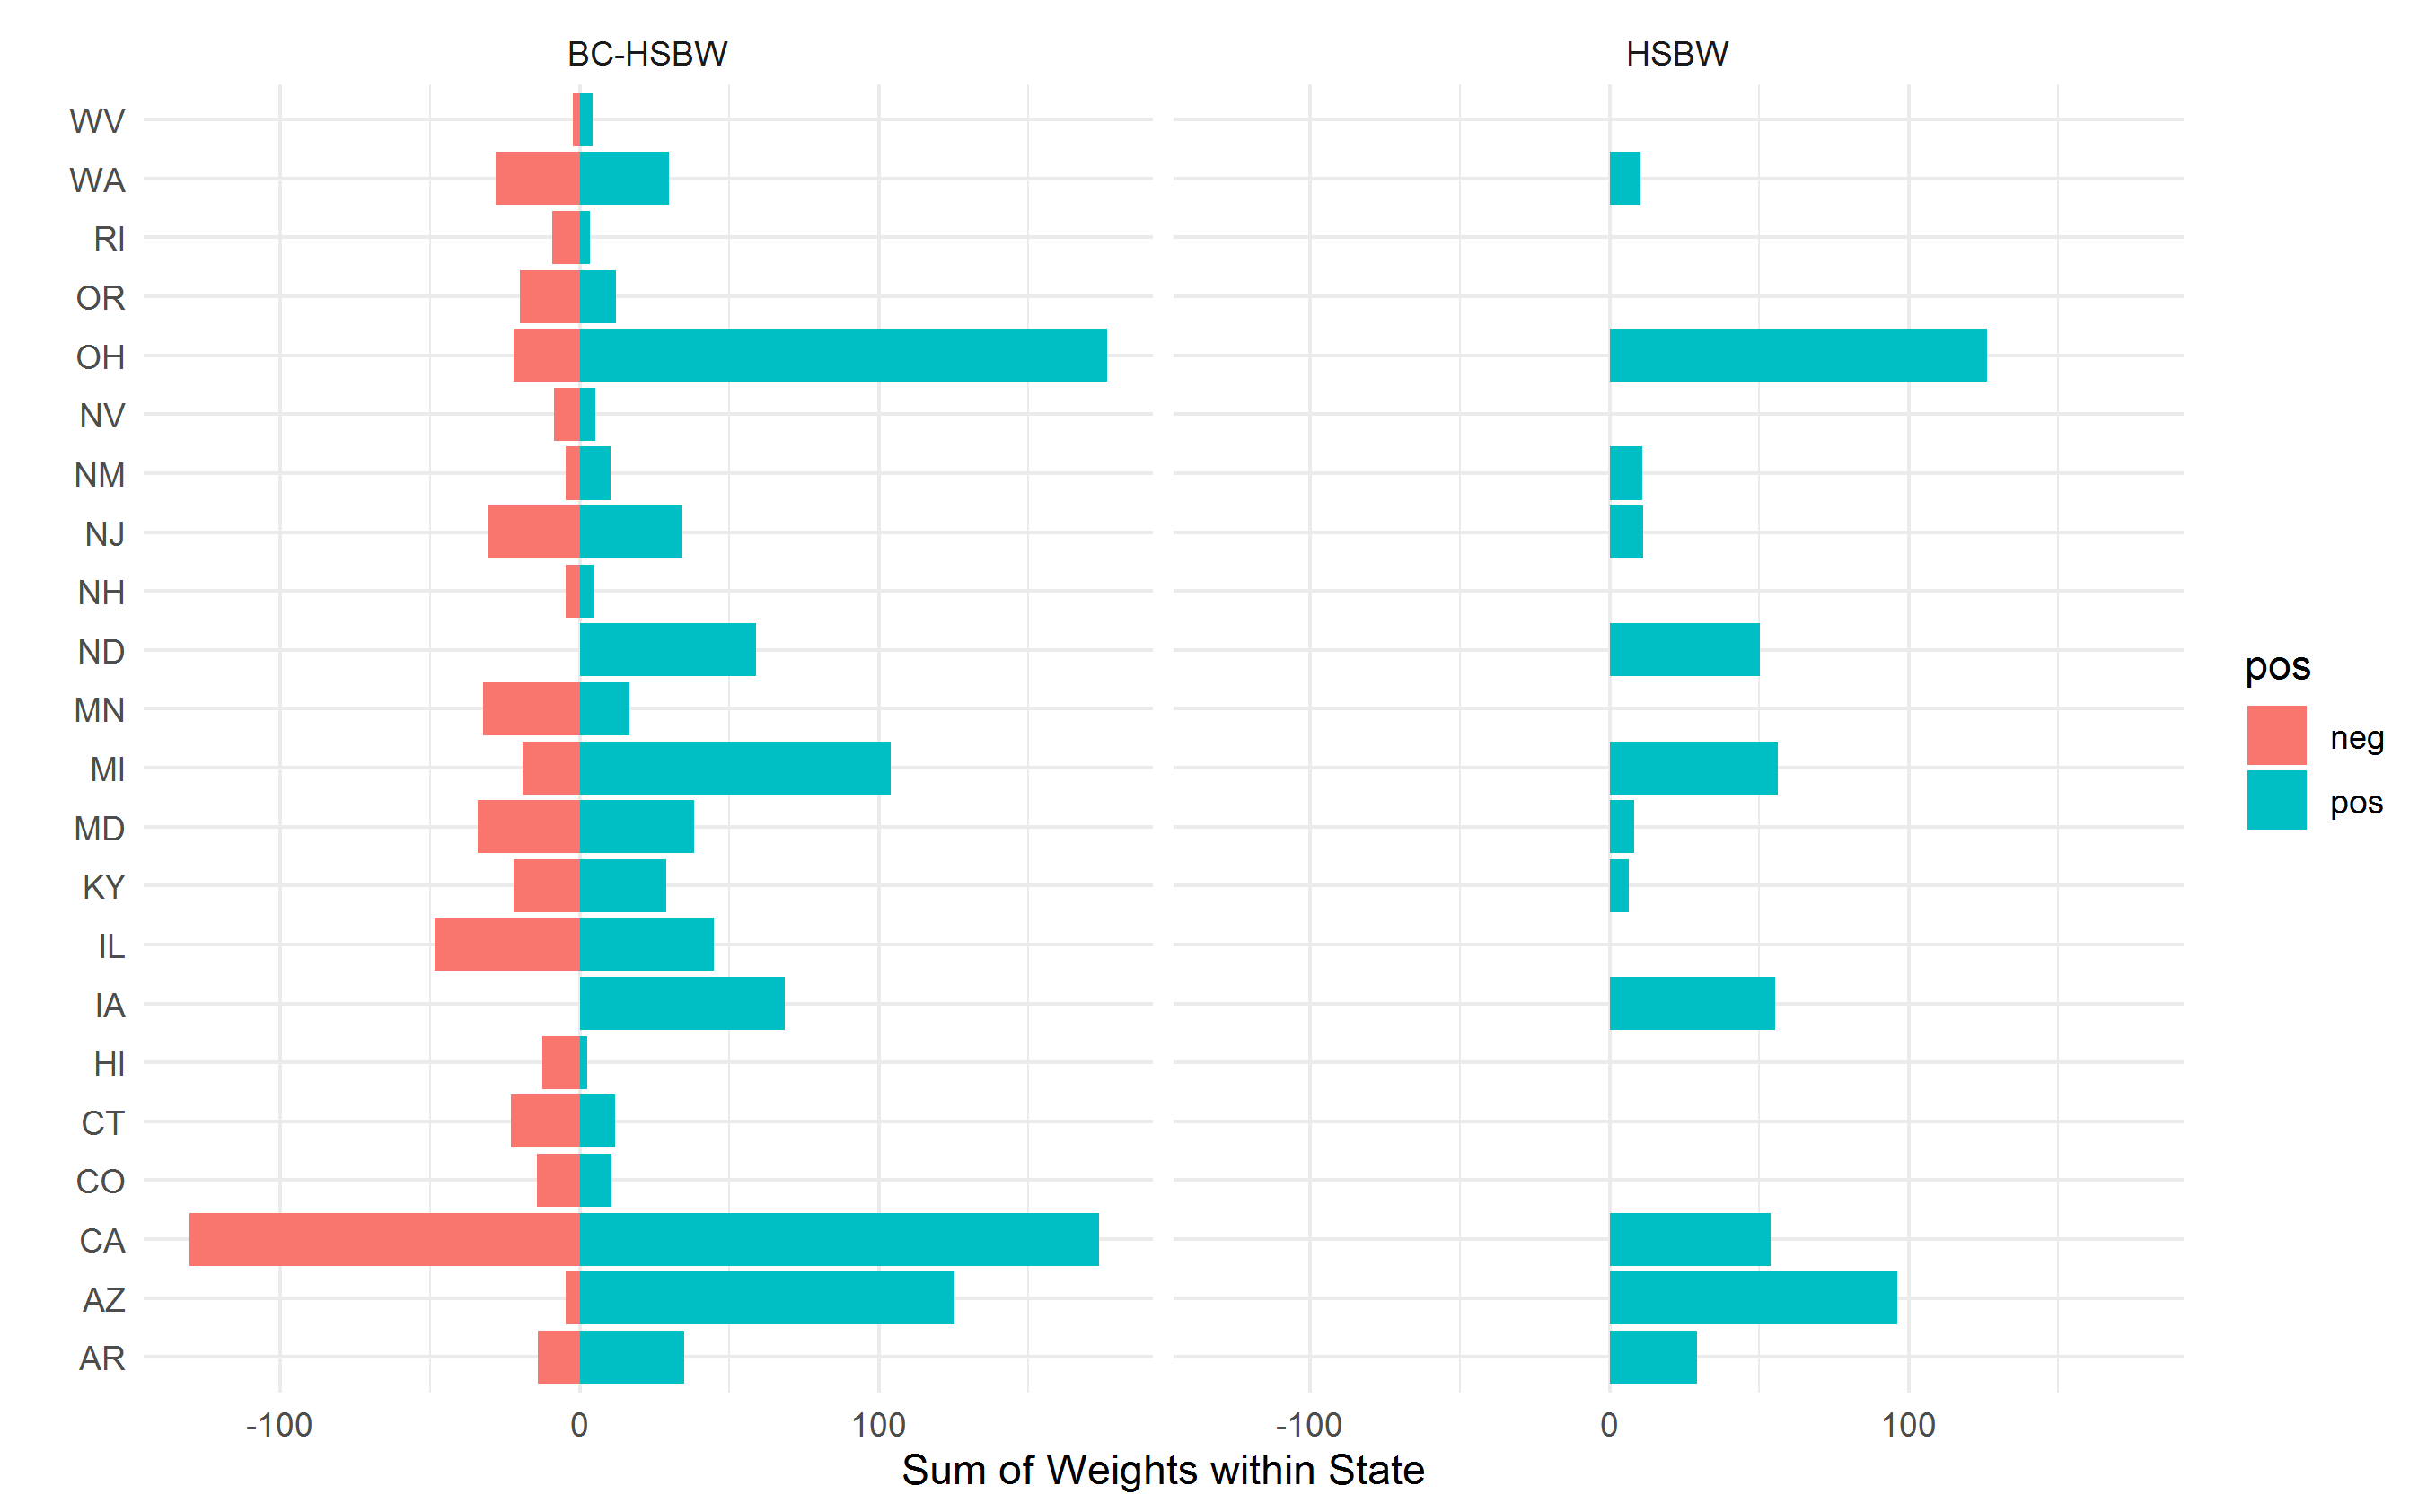
\includegraphics[scale=0.6]{01_Plots/weights-by-state-main.png}
    \caption{Total weights summed by state}
    \label{fig:statewghts}
\end{center}
\end{figure}

Our H-SBW estimator yields an estimated effect of -2.00 (-3.59, -0.40). The bias-correction makes little substantive difference, yielding an estimate of -2.14 (-3.57, -0.71). In other words, we estimate that had states that did not expand Medicaid in 2014 done so, they would have seen a 2 percentage point reduction in their uninsurance rates that year. These estimates differ somewhat from the estimates we find running the procedure on our unadjusted covariate estimates: here H-SBW gives an estimated effect of -2.26 (-3.23, -1.29), and the bias corrected estimator yields -2.50 (-3.41, -1.58). Using the adjusted covariate set appears to both move our estimate closer in absolute magnitude towards zero and increase the width of the estimated confidence intervals. Figure~\ref{fig:estimators} displays the point estimates from these weighting estimators, as well as estimators using SBW, on the adjusted and unadjusted datasets. We also calculate estimates using Oaxaca-Blinder (regression) weights and using a second covariate adjustment; these results are substantively similar and are available in Appendix D. 

\begin{figure}[B]
\begin{center}
    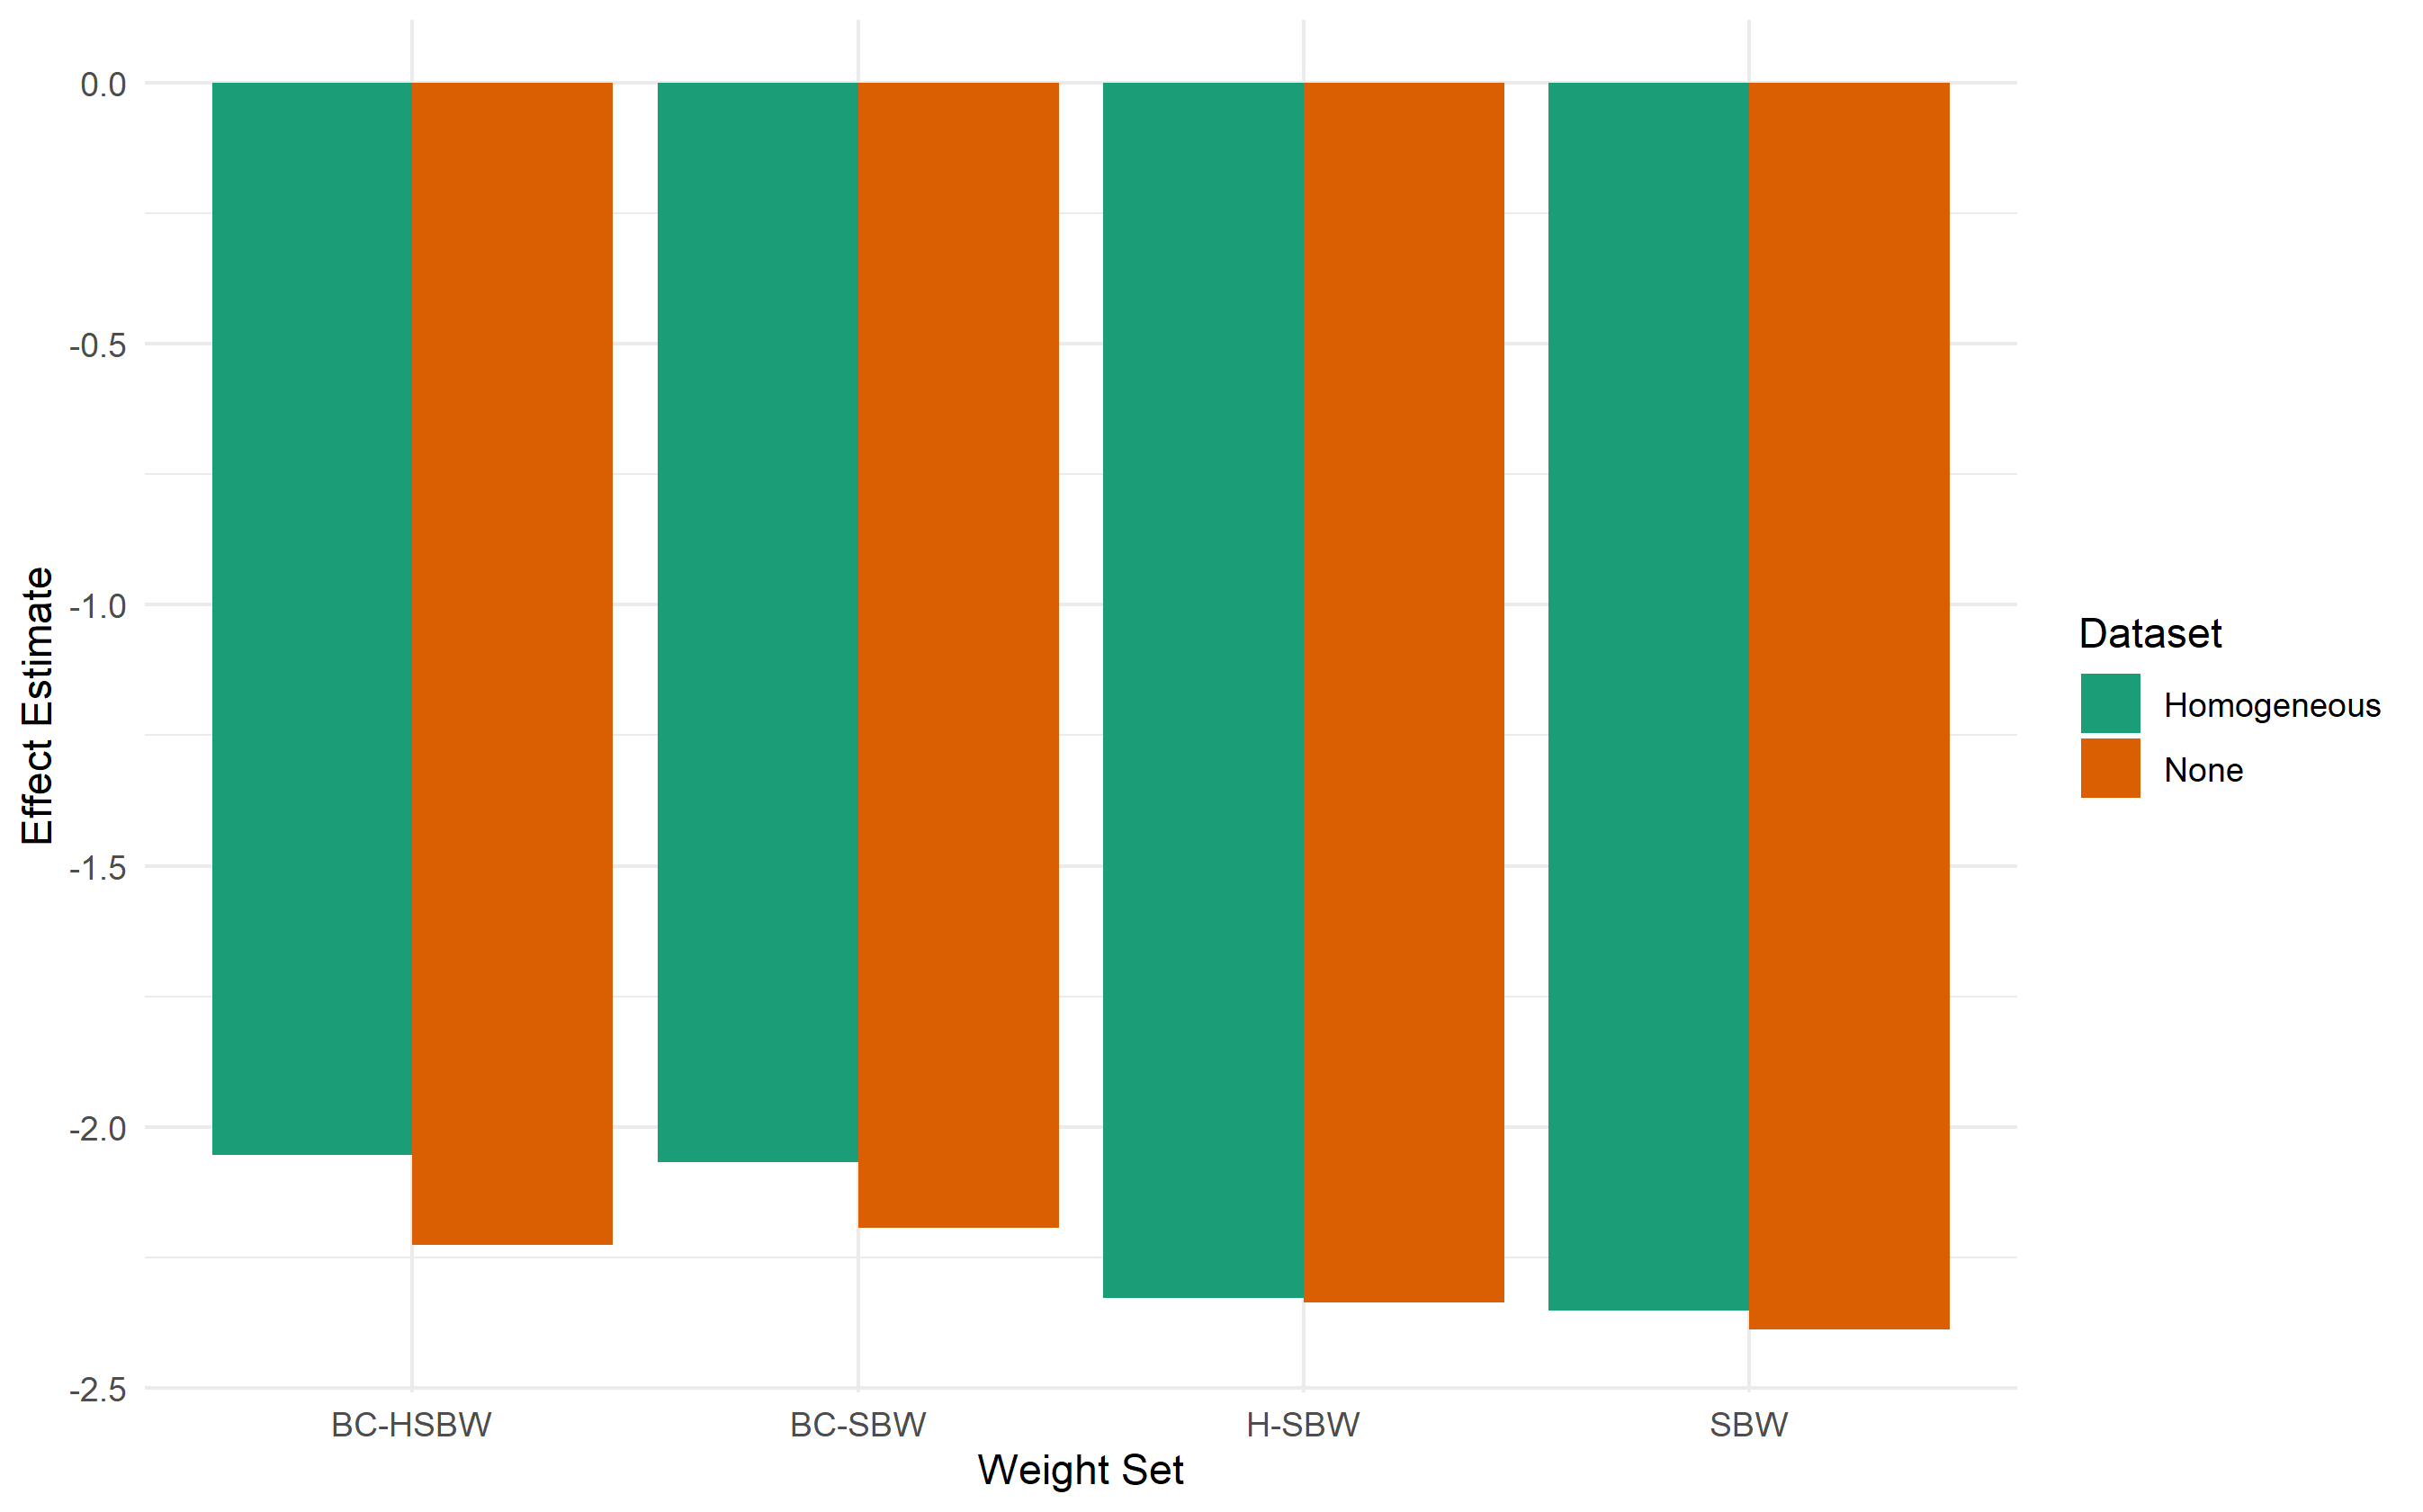
\includegraphics[scale=0.6]{01_Plots/point-estimates-c1.png}
    \caption{Point estimates}
    \label{fig:estimators}
\end{center}
\end{figure}

We next examine how removing specific covariate groups in the weighting procedure changes the estimated contrast between the weighted treatment and control regions' outcomes (ie the estimated treatment effect when all groups are included). We are especially interested in how this contrast changes when we remove the Republican governance indicators: because we hypothesize that regions under Republican governed administrations will have lower Medicaid take-up rates, we expect that removing these covariates will move this estimate farther away from zero. We divide our covariates into six separate groups: pre-treatment uninsurance rates and pre-treatment unemployment rates, Republican governance indicators, and three sets of different demographic indicators. Specifically, the first group includes: urban residence, age group, education, citizenship, student, disability, female; the second, white race, Hispanic ethnicity, foreign-born, and income-to-poverty ratio; the third, number of children, household to population ratio, and population growth. We then rerun the analyses excluding each group. 

\begin{figure}[]
\begin{center}
    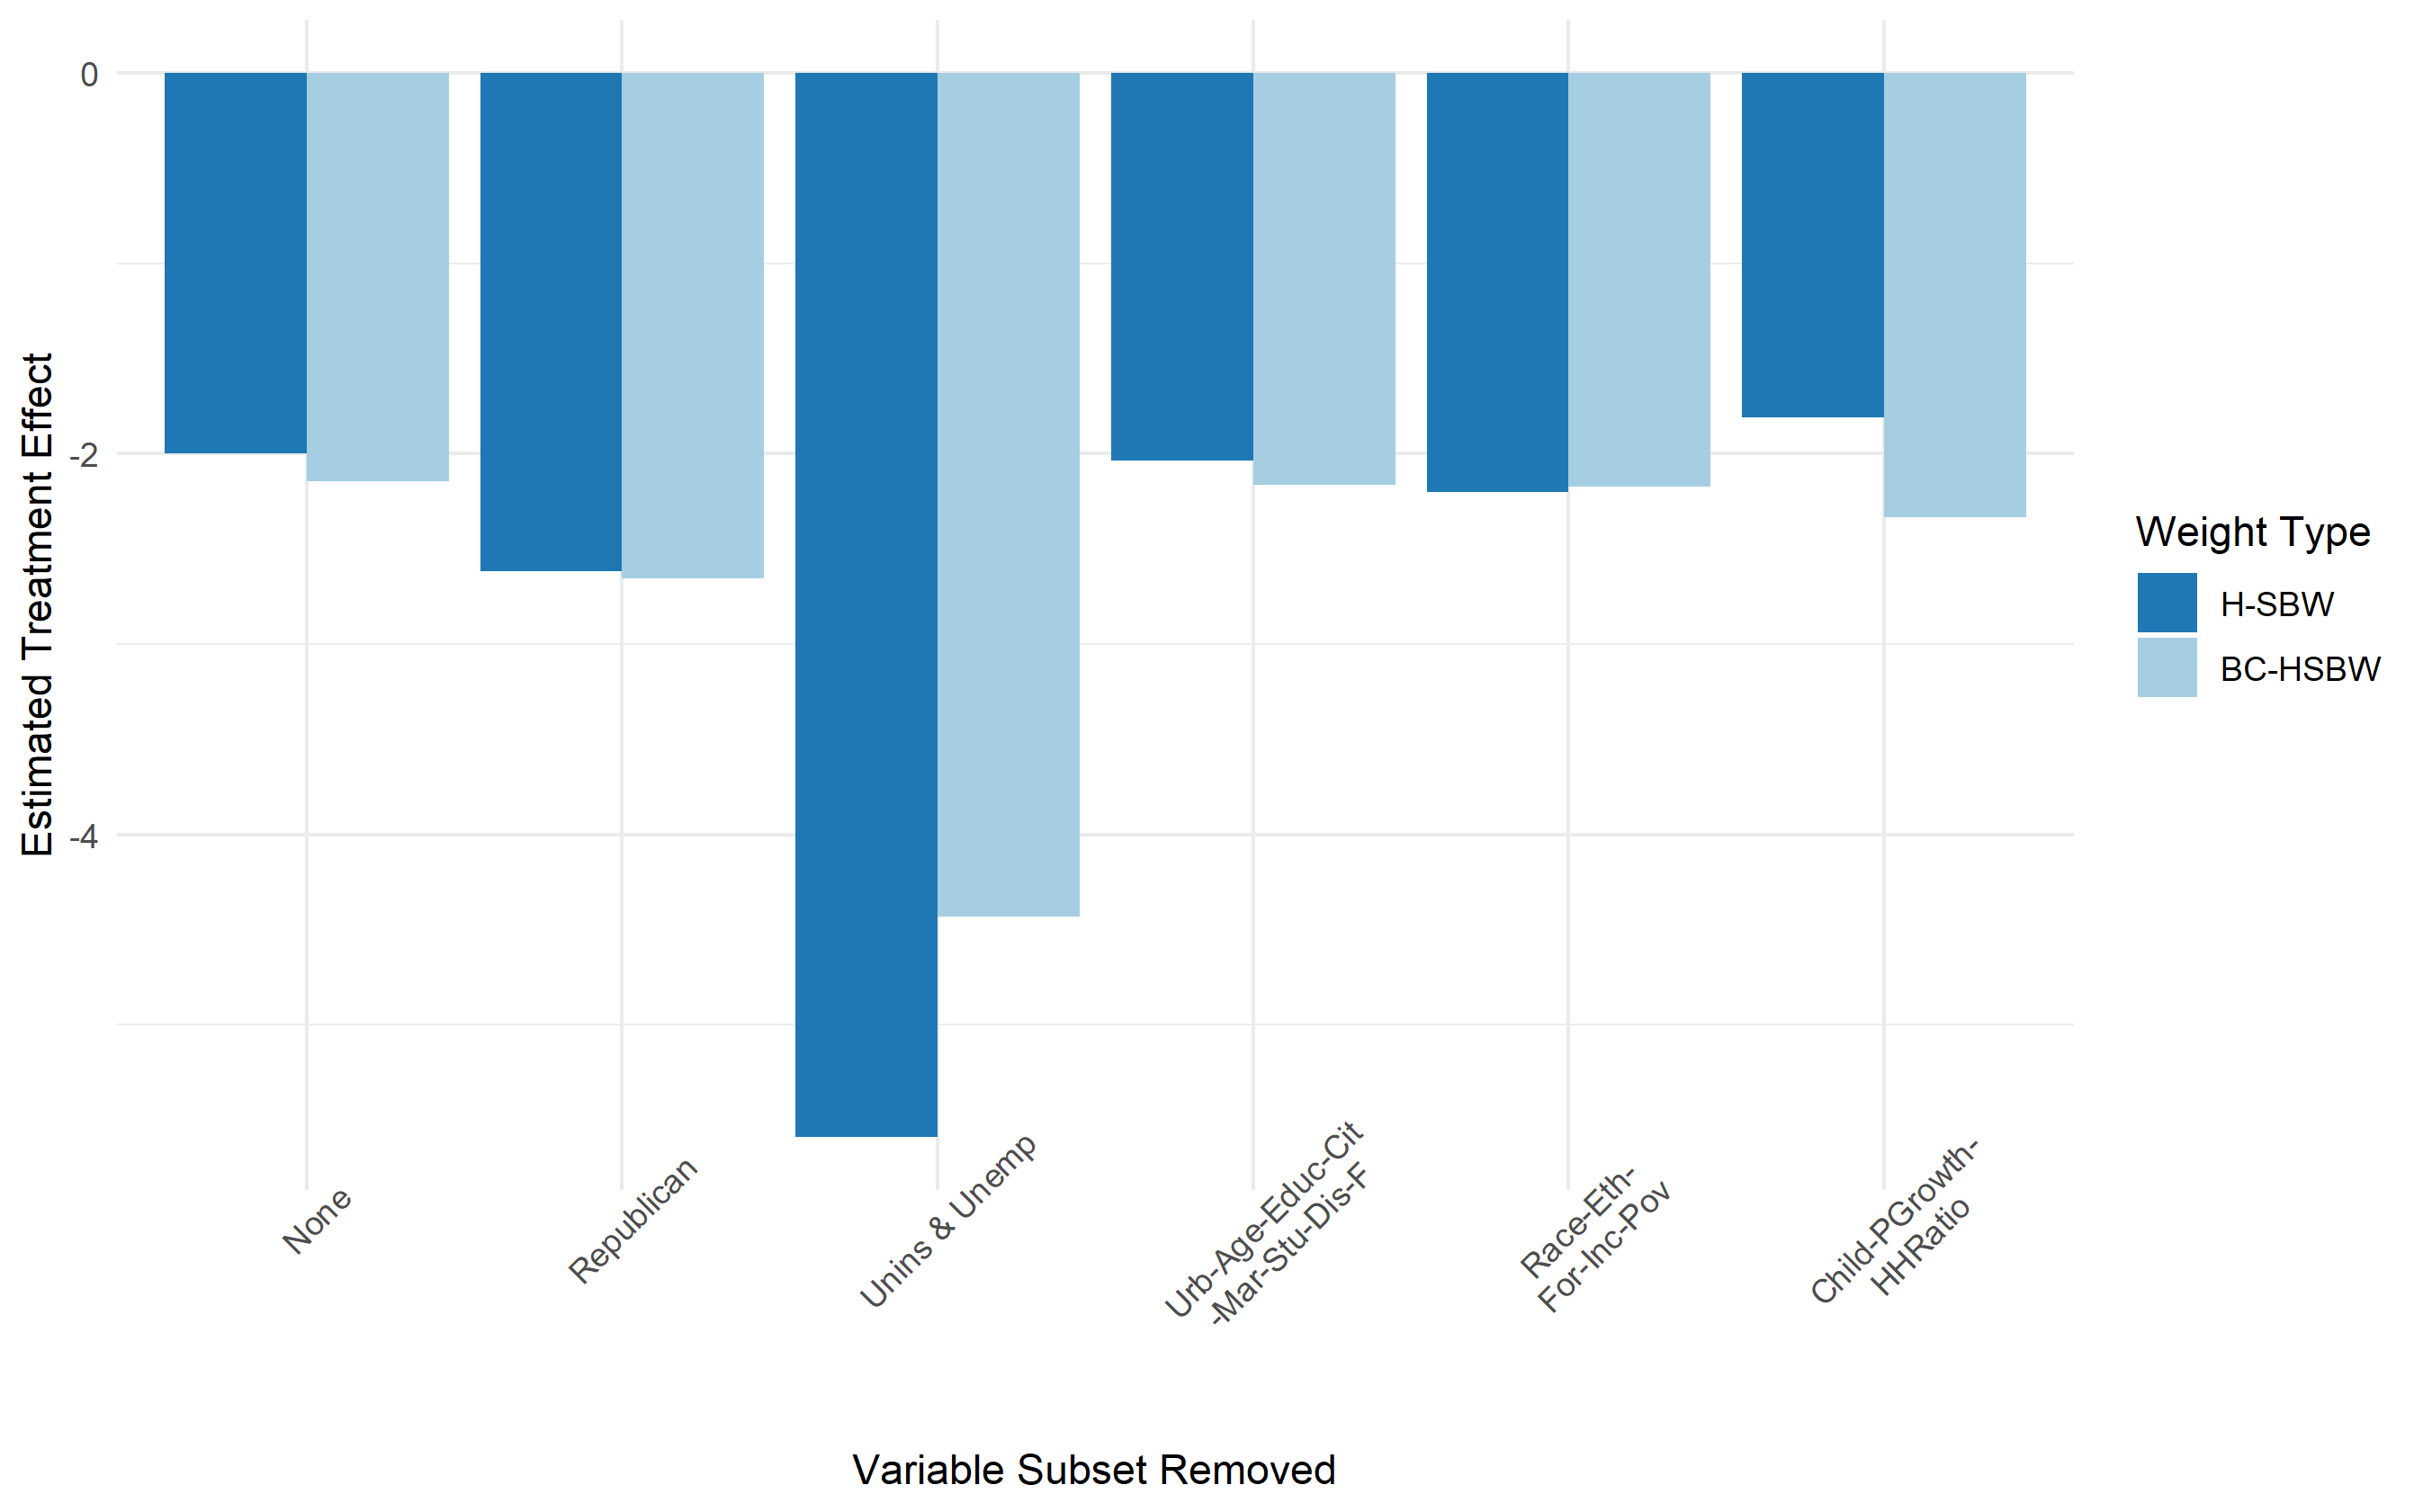
\includegraphics[scale=0.6]{01_Plots/loo-covariates-main-c1.png}
    \caption{Estimates}
    \label{fig:loocovariates}
\end{center}
\end{figure}

Figure~\ref{fig:loocovariates} displays the estimated treatment effects when removing each covariate group for our preferred set of weights and the bias corrected version of these same weights. We find that all our estimates are very sensitive to the removal of pre-treatment uninsurance and pre-treatment unemployment rates. When we fail to control for these covariates, our estimated contrast increases substantially in absolute magnitude. A full comparison of the difference in estimates across covariate groups is available in Appendix D, Table~\ref{tab:ptests}.

We also see an increase in absolute magnitude of our estimated contrast when removing the Republican governance indicators. Specifically, we find that our estimated contrast increases in absolute magnitude by 0.62 for H-SBW and by 0.51 BC-HSBW. We see similar differentials on our unadjusted dataset (0.64 and 0.49, respectively). These results are consistent with our hypothesis that Republican governance drives heterogeneity in the treatment effects. When we use the leave-one-out jackknife to calculate the standard errors of these differences, we are unable to conclude that these differences are statistically significant. Even so, we find that these differences are negative for all estimators we consider when removing each state. That is, the sign of the differences in the contrasts remains negative for every specification that we run -- conditional on the adjustment. When we re-run the entire adjustment procedure when removing each state, we do find that removing California results in a positive contrast between these estimates for BC-HSBW and BC-SBW and Illinois for BC-SBW for our adjusted dataset. However, this result does not occur with any set of weights that does not extrapolate beyond the support of the data. Figure REF displays the differences in these contrasts for our preferred adjustment dataset and our unadjusted dataset, conditional on the adjustment. Additional results are available in Appendix D, Table REF.

Finally, we consider the robustness of our estimators to the removal of individual states. Figure~\ref{fig:loostateplot} shows how the point estimates change for leave-one-state-out jackknife procedure for both the adjusted and unadjusted datasets. We see very similar results in both cases: removing Ohio and Arkansas tends to increase the absolute magnitude of the point estimates. By contrast, removing California decreases the absolute magnitude of the estimators that are not bias-corrected, but this goes away or even reverses when including the bias correction. The results are quite similar when using different covariate adjustments and when recalculating the entire procedure; some are available in Appendix D, Table~\ref{tab:sensitivityc1}. 

\begin{figure}[]
\begin{center}
    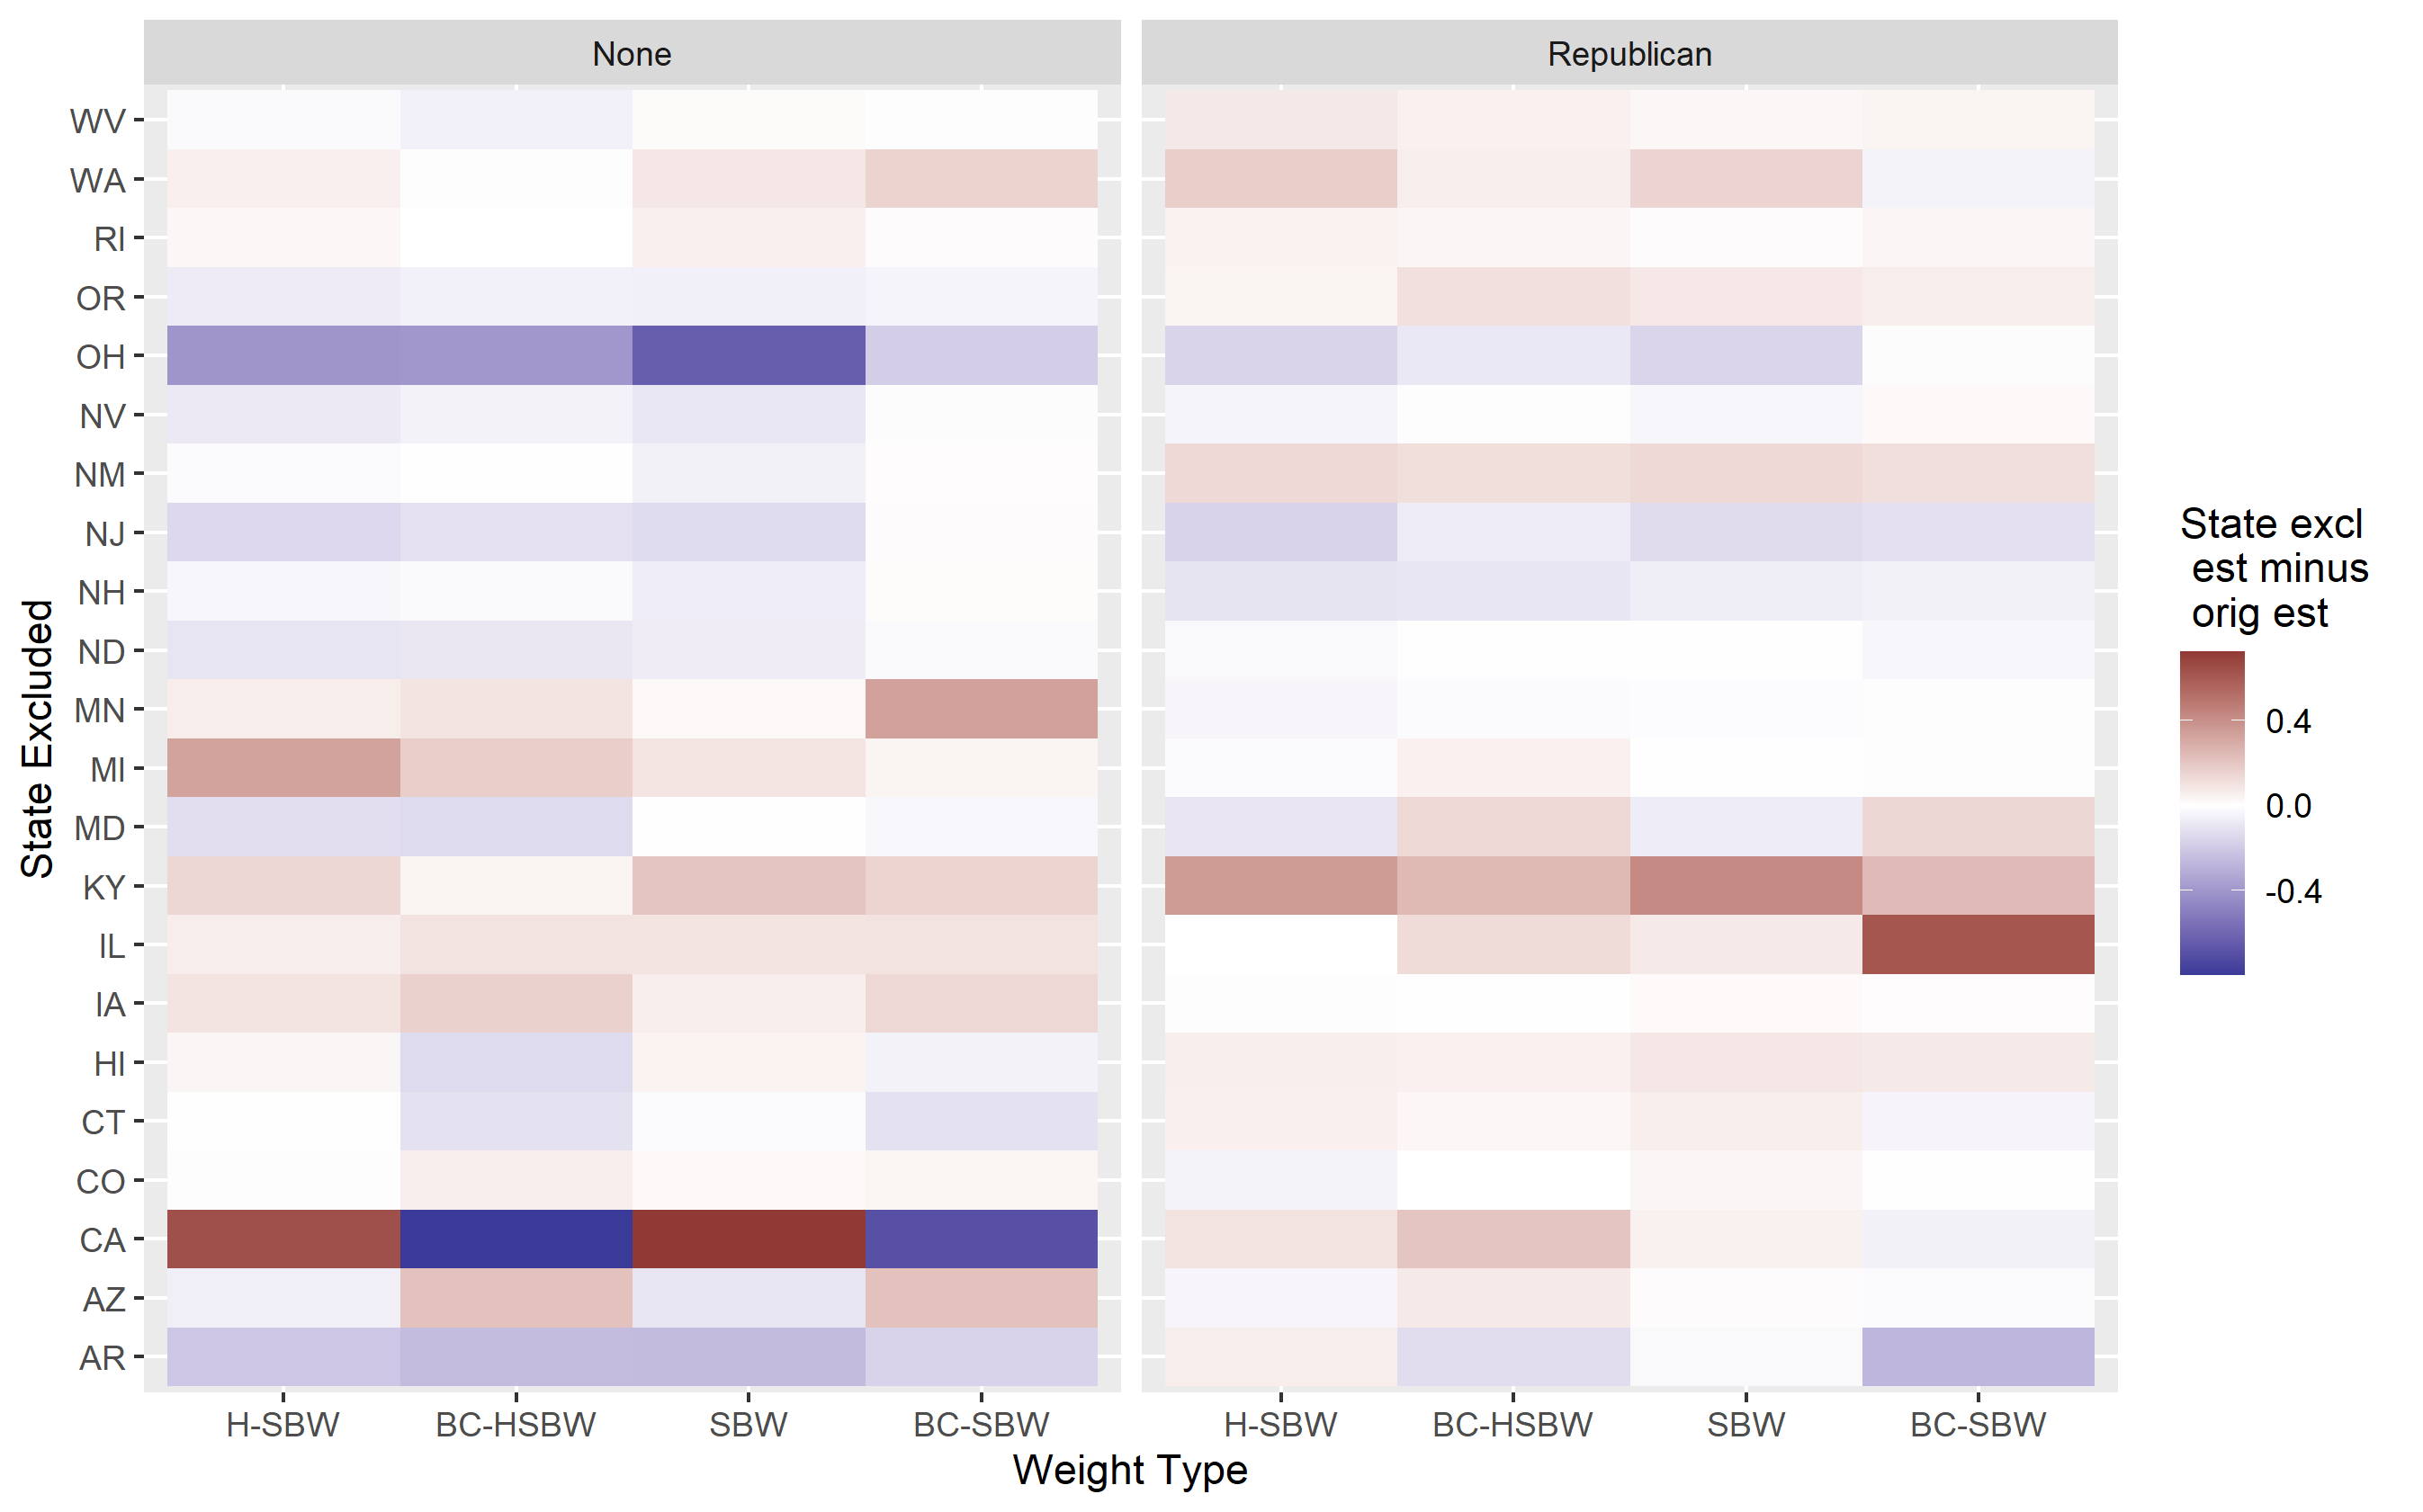
\includegraphics[scale=0.6]{01_Plots/c1-loostate-sensitivity.png}
    \caption{Estimator sensitivity to states}
    \label{fig:loostateplot}
\end{center}
\end{figure}

\subsection{Sensitivity Analyses} \label{sssec:sensitivity}

We examine the sensitivity of our estimates to violations of two key causal assumptions: (1) no anticipatory treatment effects, and (2) positivity violations. To the first point, several states had partial limited expansions prior to 2014. Following \cite{frean2017premium}, we consider these states to be California, Connecticut, Minnesota, New Jersey, and Washington. We rerun our analyses excluding CPUMAs from all five of these states. It is unclear how removing these states might affect our estimates: on the one hand, states that expanded early might have a smaller treatment effect after 2014 because they already enrolled newly eligible individuals. On the other hand, if these states were also more motivated to enroll people in Medicaid, they might have larger post-expansion coverage gains. When removing these states, we estimate an effect of -1.29 (-2.45, -0.12) using H-SBW weights and when we run the bias-corrected version we estimate -2.17 (-3.65, -0.68). While these point estimates are quite a bit different but the confidence intervals largely overlap. Table~\ref{tab:secondaryptests} in Appendix D displays additional results. 

Our leave-one-out covariate analysis shows similar associations to those in our primary analysis; however, we see a somewhat larger association between Republican governance indicators and our estimated contrast. Specifically, we find a 1.28 percentage point increase in absolute magnitude when for the H-SBW estimator and a 0.73 increase for BC-HSBW. Figure~\ref{fig:repub} displays these differences in the contrasts against those from our preferred dataset. 

\begin{figure}[]
\begin{center}
    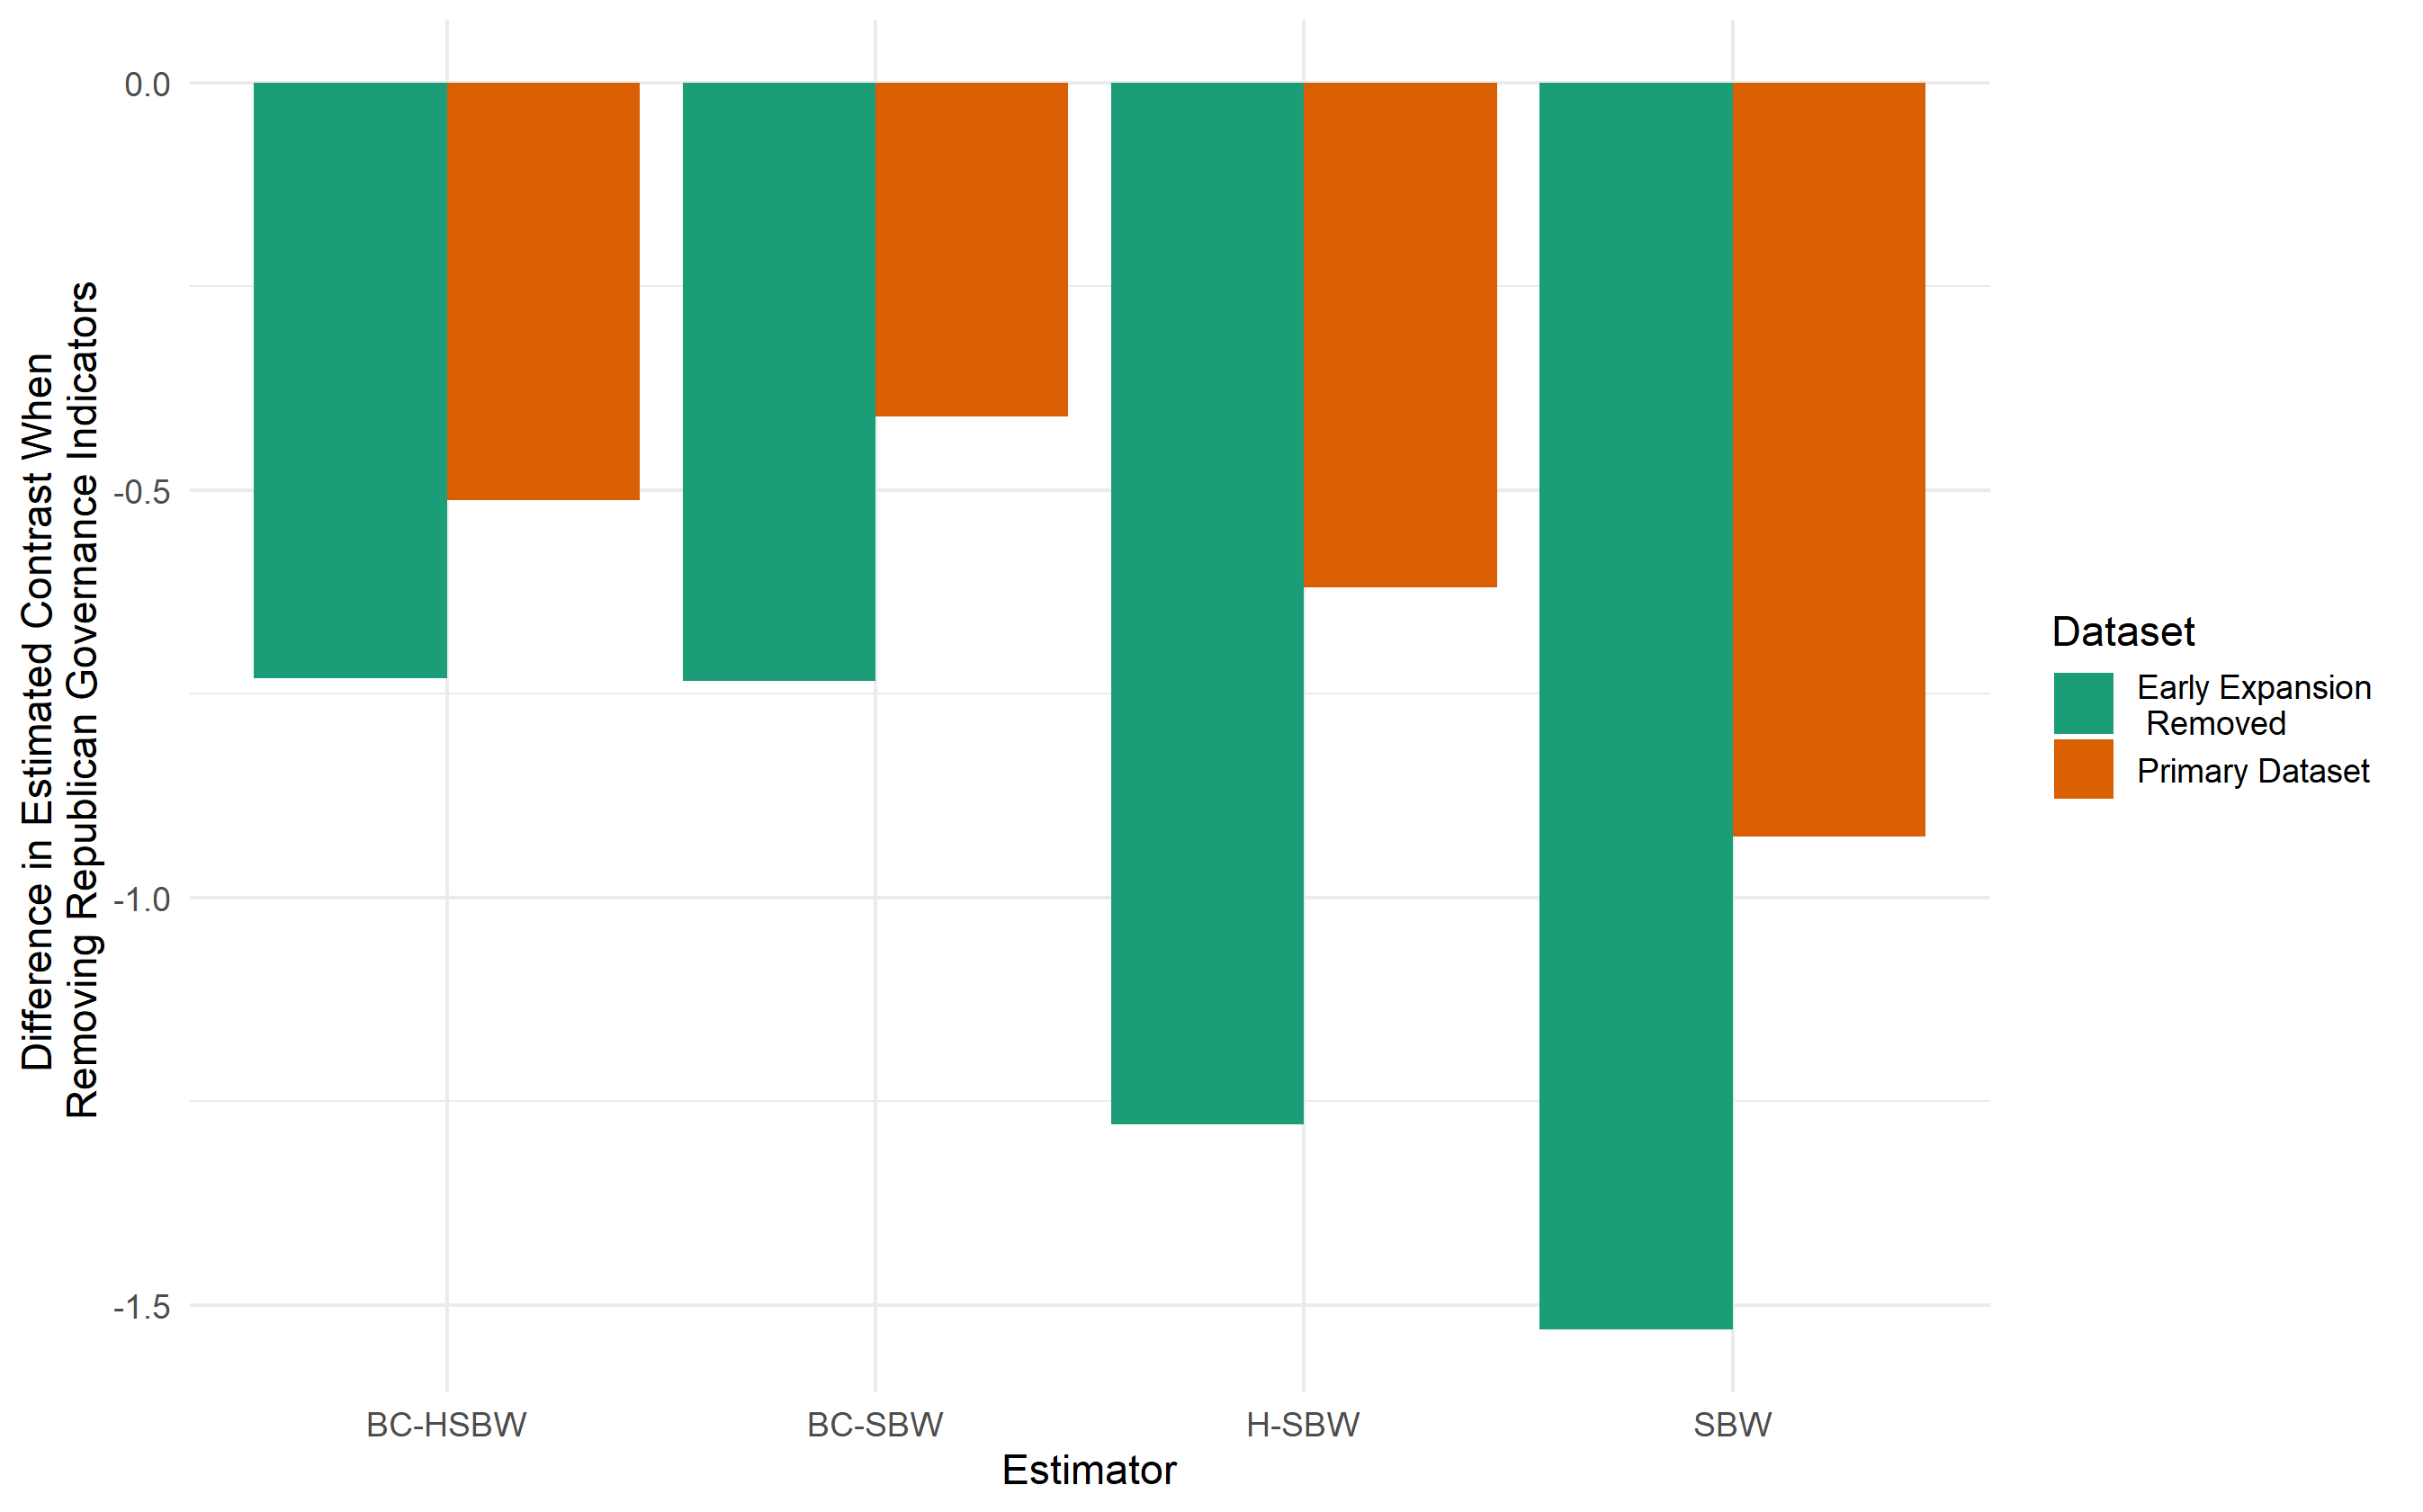
\includegraphics[scale=0.6]{01_Plots/repub-diff-c1c2.png}
    \caption{Removing Republican Governance Indicators}
    \label{fig:repub}
\end{center}
\end{figure}

When we compute the leave-one-out jackknife standard errors, we find that the estimates for H-SBW and SBW are statistically significantly different from zero on both the adjusted and unadjusted datasets (H-SBW (-2.19, -0.35); SBW (-2.30, -0.75)). This result also holds when calculating these contrasts when recalculating the entire procedure. We again find that for all estimators (including the Oaxaca-Blinder weights), the difference between the leave-one-out-states estimated contrasts are negative conditional on the preferred covariate adjustment. When we rerun the entire adjustment procedure, we again find that the only estimators that have positive differences between these contrasts are ones that allow for negative weights. For our preferred covariate adjustment, BC-HSBW and BC-SBW are only sensitive to the removal of Kentucky. Additional results are available in Appendix D, Table BLAH. 

We next consider an alternative method to account for positivity violations. To this point we have relied on either (1) retaining a potentially biased estimate from weights that do not provide exact balance, or (2) producing a a more model-dependent estimate that relies on extrapolation. Overall we found that the results didn't change substantially either way. Here we consider a third option: changing our target estimand. In particular, we consider the overlap average treatment effect (OATE), proposed by \cite{li2018balancing}. This is the treatment effect on the subset of the entire dataset where we have overlap. It is a data-dependent treatment effect, and is not the same as the treatment effect on the untreated; however, we believe that this effect will be more similar to the ETC than the ETT, since there were no Democratic controlled states that did not expand Medicaid. Indeed, after generating overlap weights on our primary dataset we find that across all covariates, the mean average absolute distance from the overlap region to the untreated region is 2.9 and to the treated region is 7.8.\footnote{The distance is between the overlap region calculated as an unweighted mean on the adjusted datasets.} Figure~\ref{fig:oatearea} displays the distance between covariates with greater than one percentage point distance from the overlap region to either the control or treated region. We see that the overlap region is substantially more Republican than the treated region, as expected. This region is also less Hispanic, more white, less rural, and more educated than either the expansion or non-expansion region. Table~\ref{tab:oatedist1} and Table~\ref{tab:oatedist2} in Appendix C show statistics on the OATE region versus the treatment and control regions for all covariates.

\begin{figure}[]
\begin{center}
    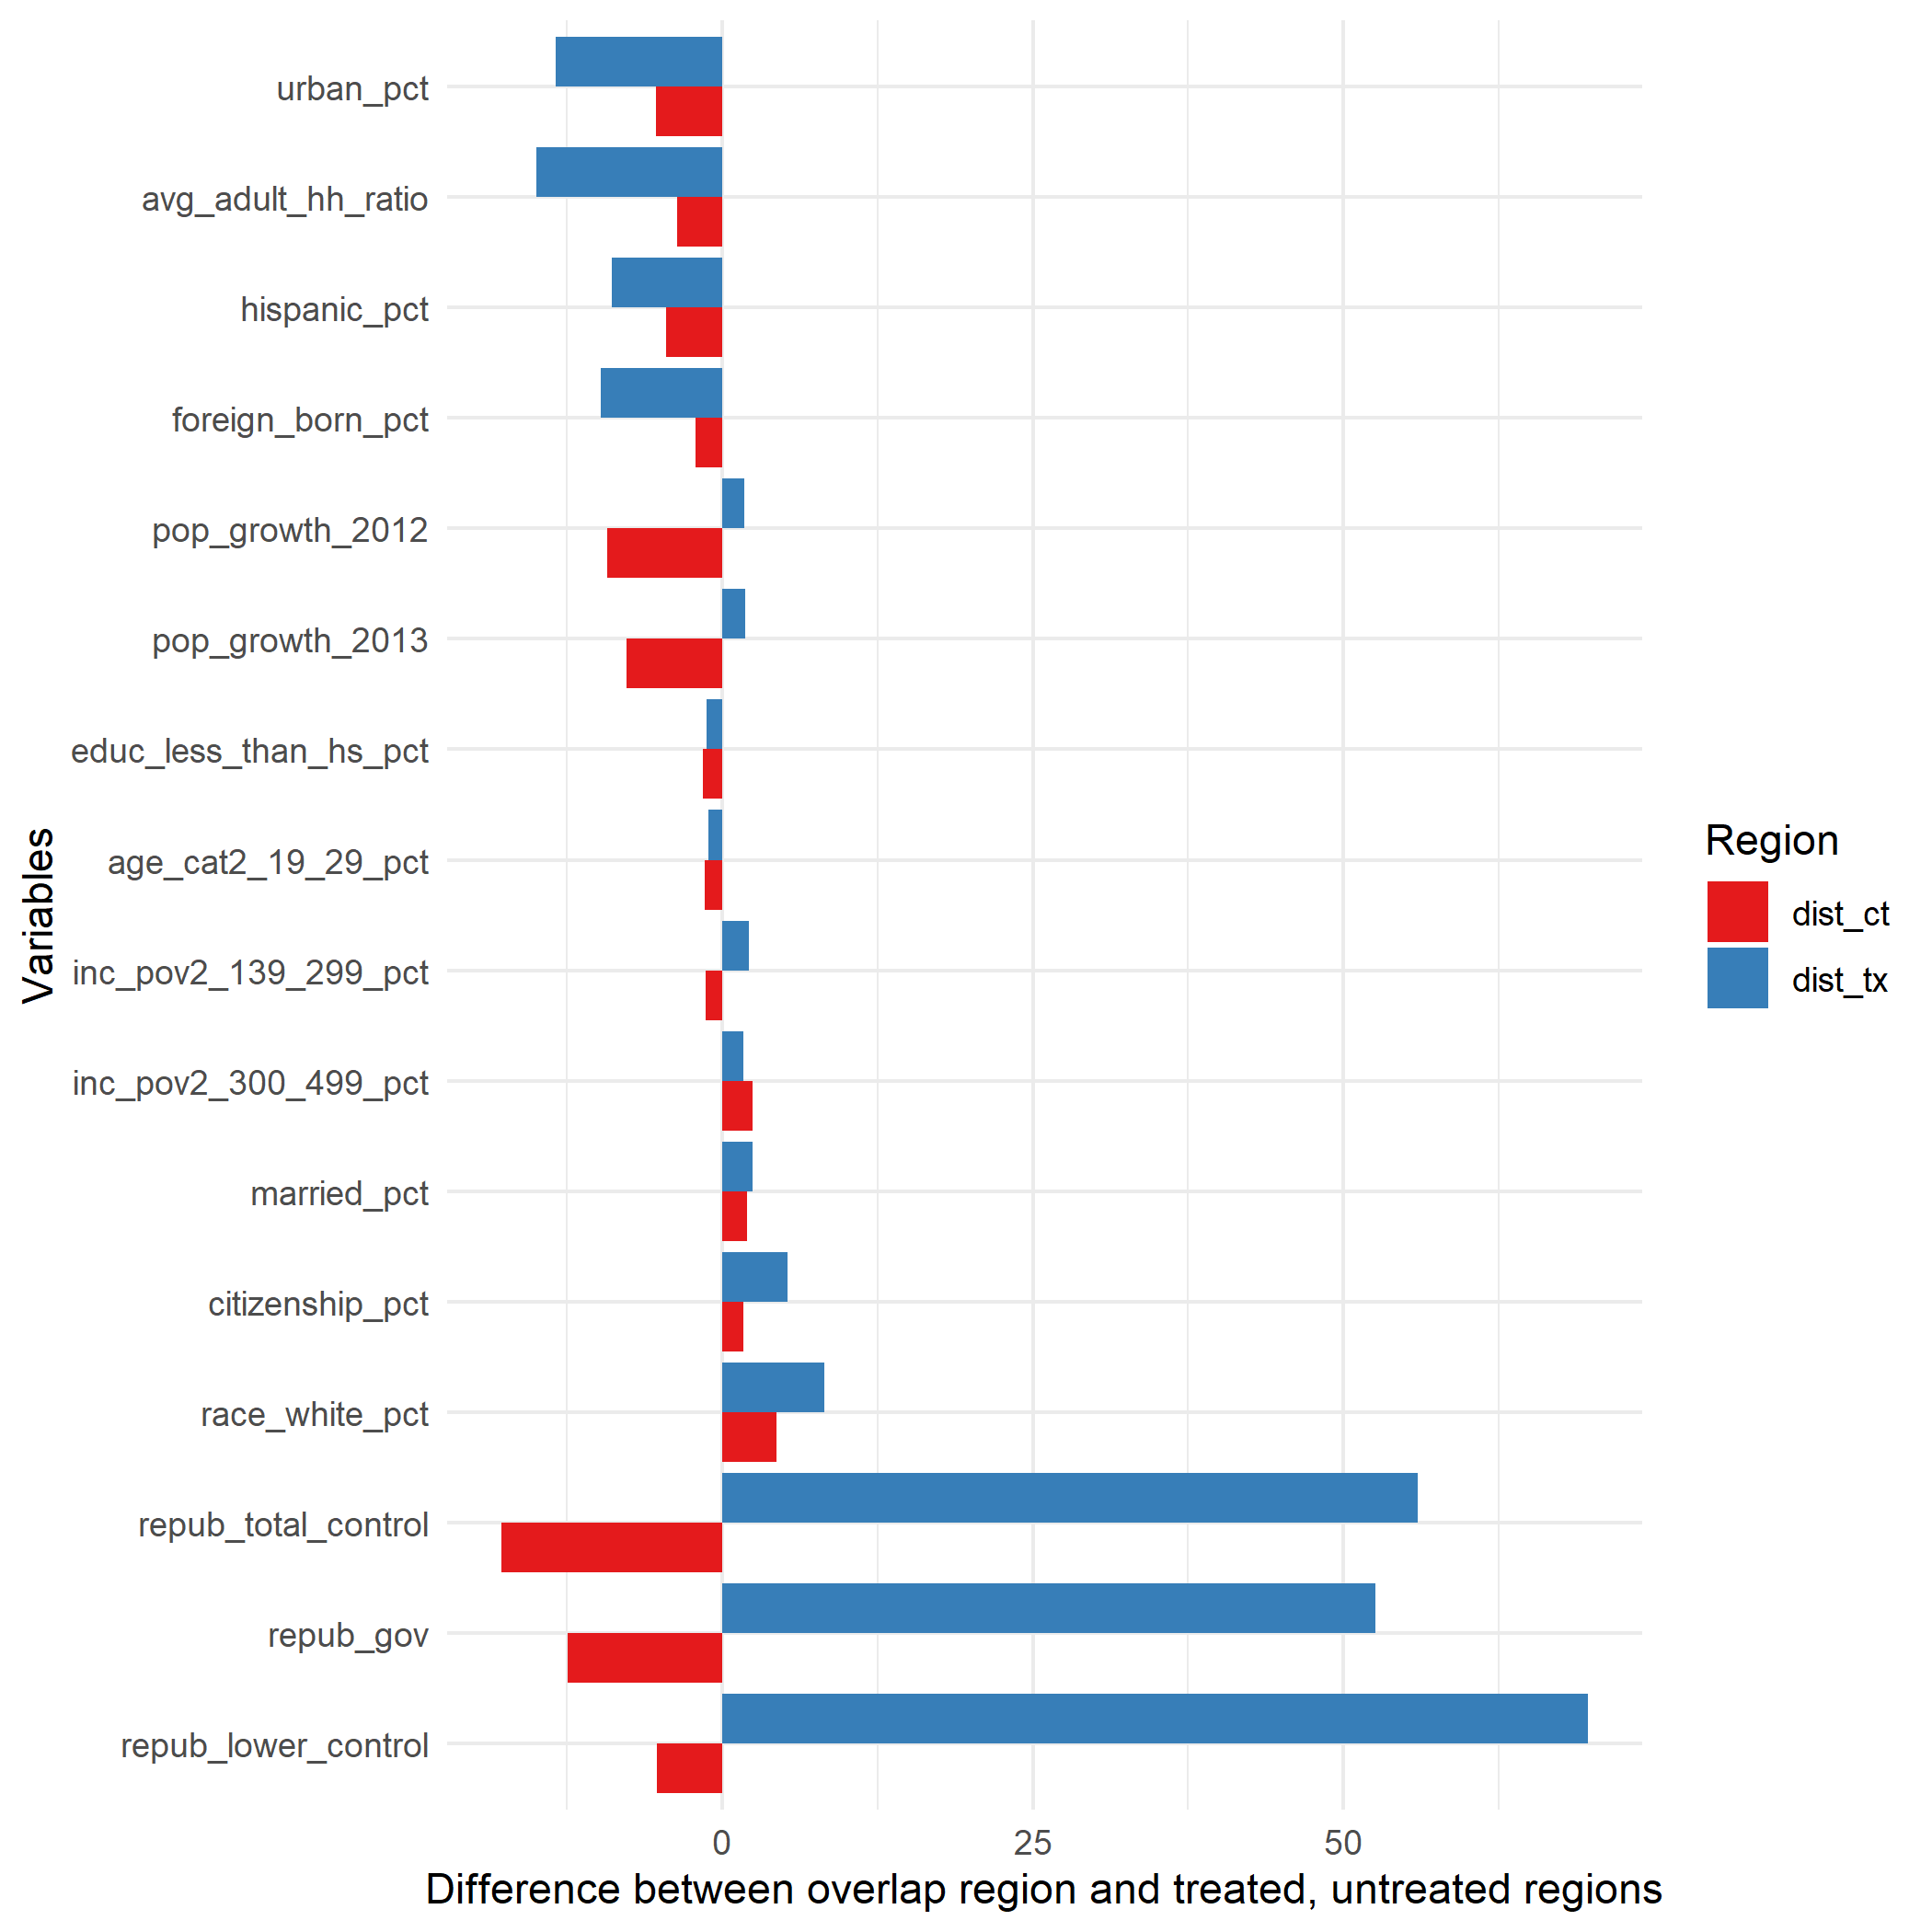
\includegraphics[scale=0.6]{01_Plots/oate-imbalances.png}
    \caption{Overlap area compared to treated, untreated regions}
    \label{fig:oateimbalance}
\end{center}
\end{figure}

Figure~\ref{fig:oateimbalance} displays the sum of the weights within each state by treatment group. Ohio, Michigan, and Arkansas, which all expanded Medicaid, are the most heavily weighted states (the weights are standardized to sum to 100). The weights are more evenly dispersed among the non-expansion regions, though Pennsylvania, Missouri, Wisconsin, and Florida are given the most weight. We note that this region is specific to the preferred covariate adjustment; the results are quite similar for the unadjusted and less preferred covariate adjustment and are available in Appendix D, Table ~\ref{tab:oatestateweights}.

\begin{figure}[]
\begin{center}
    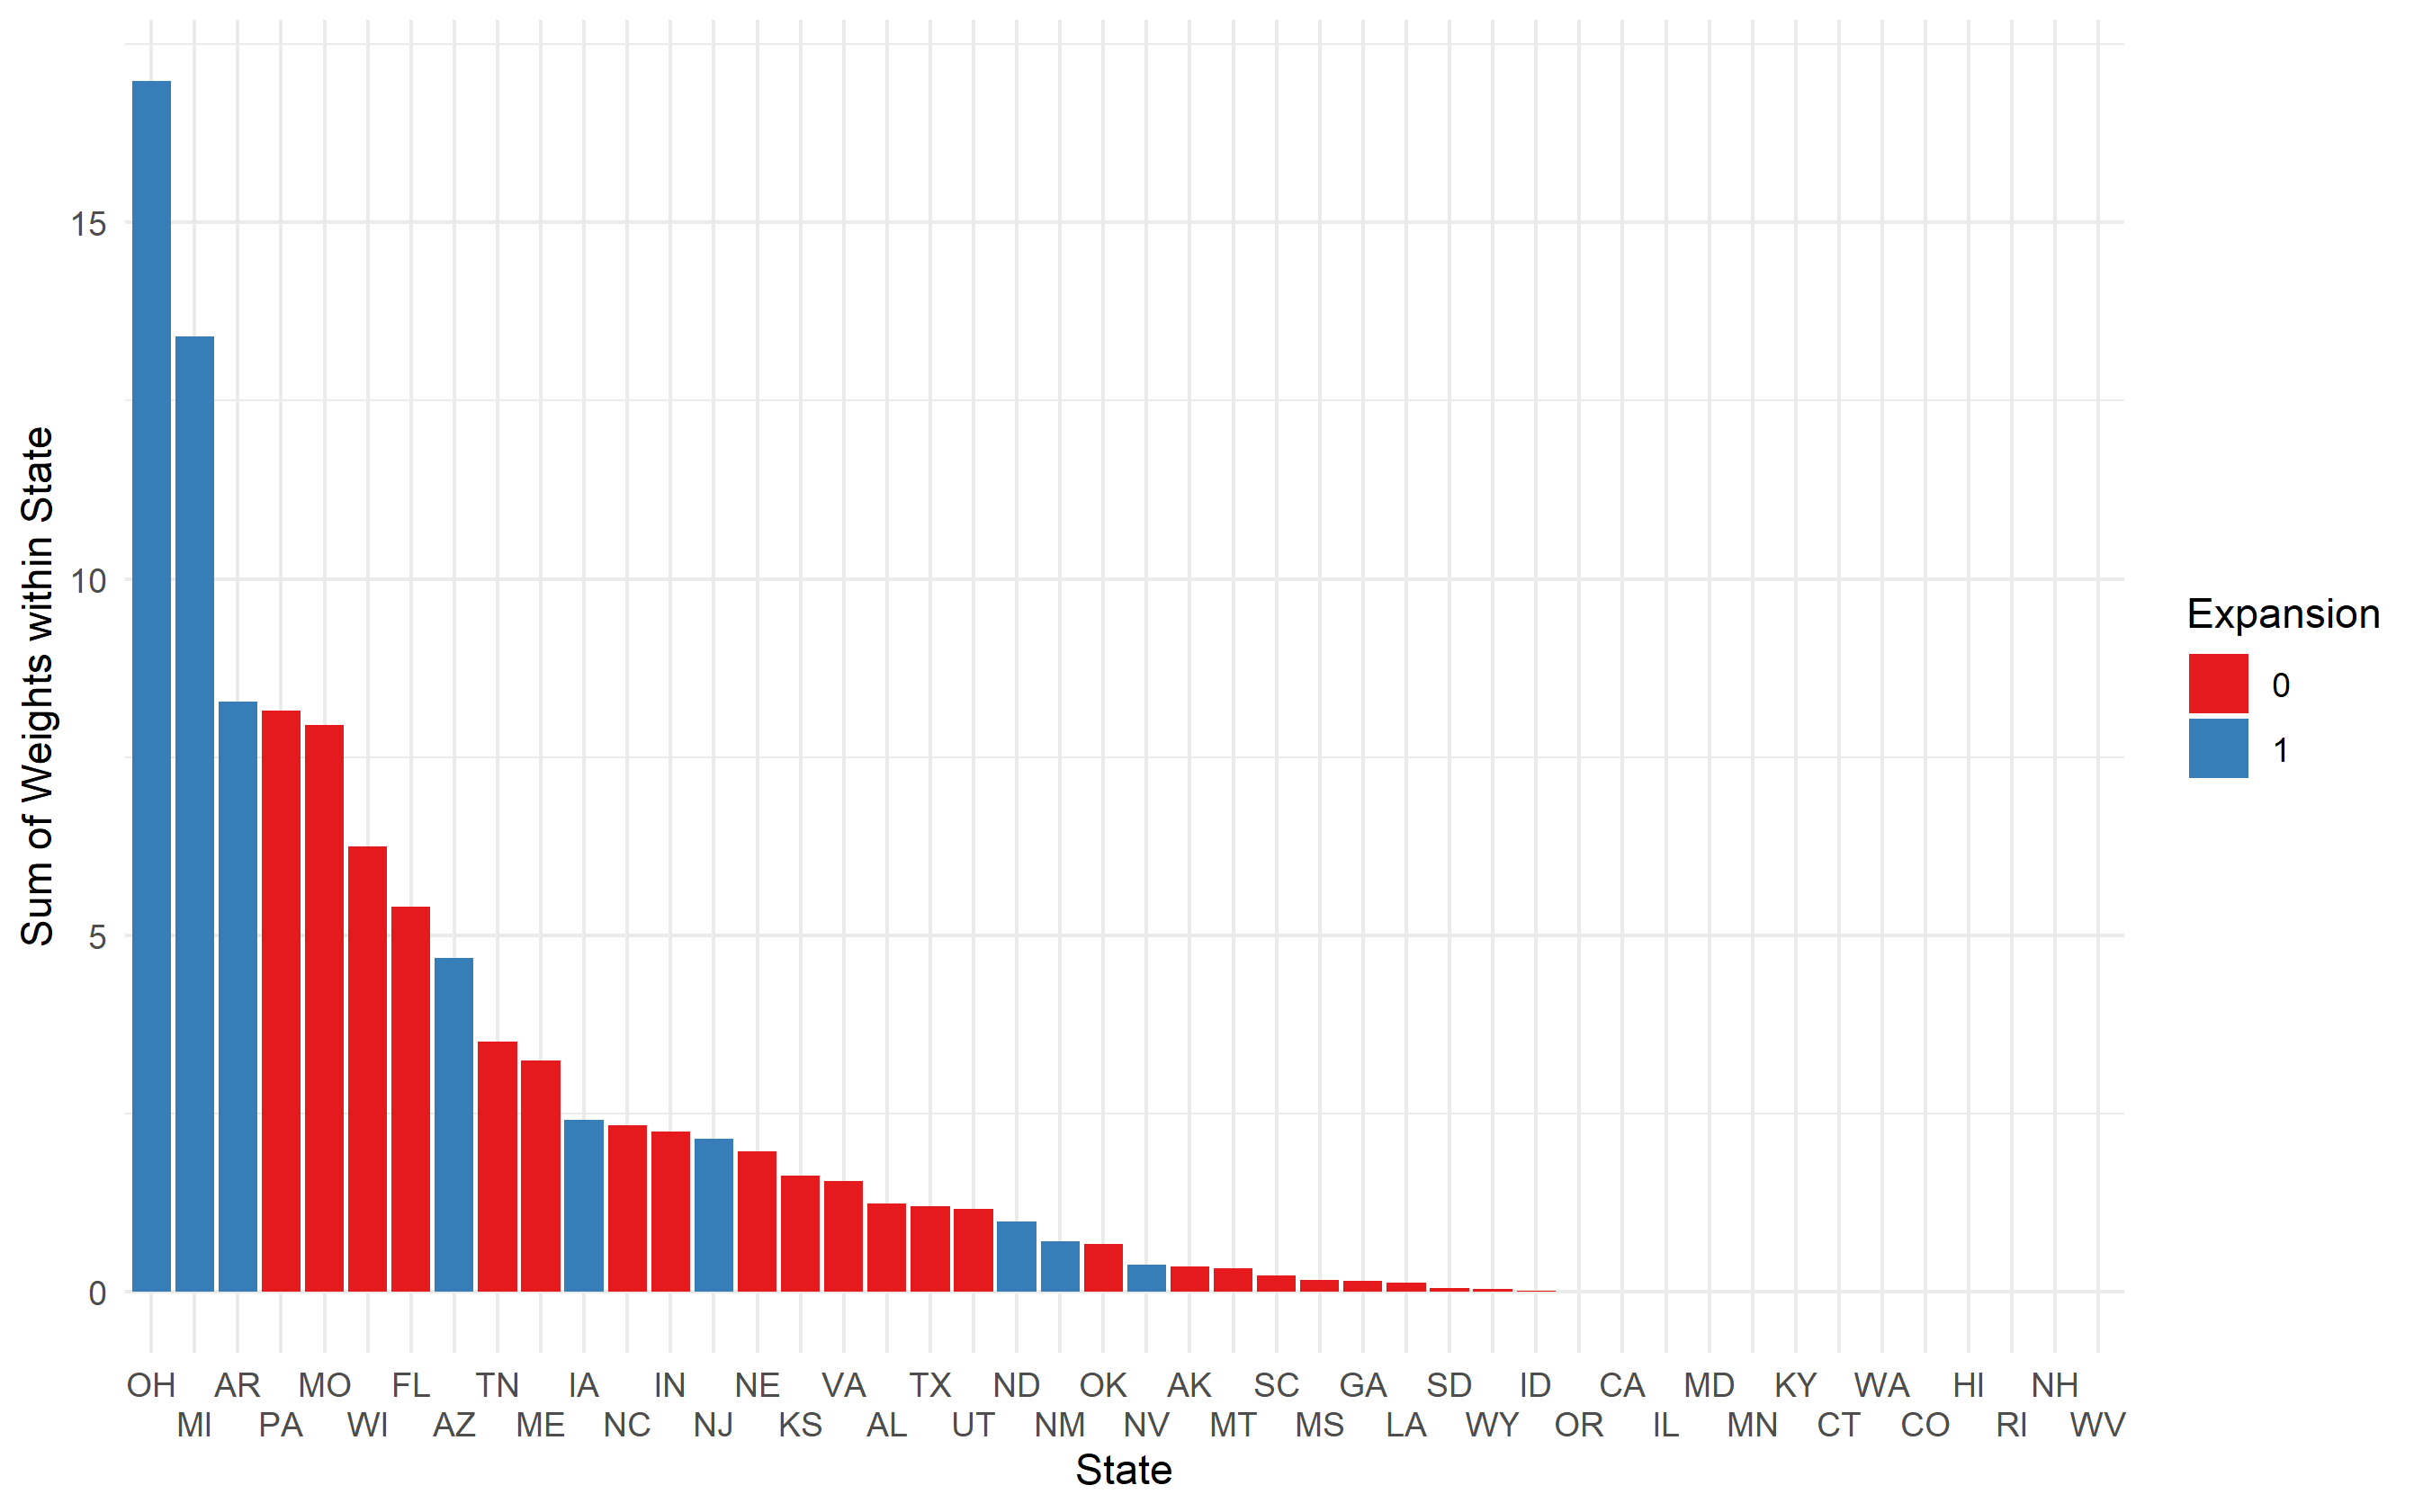
\includegraphics[scale=0.6]{01_Plots/oate-region-c1-a.png}
    \caption{Overlap weights by state}
    \label{oatearea}
\end{center}
\end{figure}

We find similar results to our primary analysis: within the overlap region we find an estimated treatment effect of -1.64 (-2.41 -0.89) when including all treatment states in our primary analysis, and of -1.76 when excluding ``early expansion'' states. We again find a negative association between the estimated contrast and the Republican governance indicators, which decrease the estimated effect size by 0.96 (0.81, 1.10) percentage points on the primary dataset and by 0.62 (0.78, 0.46) percentage points when removing early expansion states. Notice that both of these estimates were statistically significant; the confidence intervals increase only slightly when recomputing the entire adjustment when removing each state. Moreover, this negative difference in estimated contrasts holds for each state left outside, regardless of whether or not we conditioned on the adjustment or recalculated it. Additional results are available in Appendix D, Table~\ref{tab:oateconfint} and Table~\ref{tab:oatesensitive}. This again provides support for our hypothesis that Republican governance is an important predictor of treatment effect heterogeneity.

\section{Discussion}

We estimate that had states that did not expand Medicaid in 2014 expanded their programs, they would have seen a -2.14 (-3.57, -0.71) percentage point change in the adult uninsurance rate. Existing estimates place the ETT between -3 and -6 percentage points; these estimates vary depending on the targeted sub-population of interest, the data used, and the modeling approach (see, eg, \cite{courtemanche2017early}, \cite{kaestner2017effects}, \cite{frean2017premium}). This ETC estimate is therefore closer to zero than these ETT papers, supporting our original hypothesis that the treatment effect on non-expansion states would be smaller in absolute magnitude. Moreover, we also find that we are likely to estimate treatment effects that are larger in absolute magnitude when allowing our comparison states to include states governed by the Democratic party. While the differences all lay within the estimated margins of error of the original point estimates, the consistency of this finding in all of our sensitivity analyses provides evidence that the differing political composition of the expansion versus the non-expansion states may explain these differences. 

We also make several methodological contributions to the literature on balancing weights. First, we extend the synthetic controls literature to estimate the treatment effect on the controls. The key challenge is that we need to predict treatment response rather than the outcome absent treatment. Unlike when estimating the treatment effect on the treated, we cannot use pre-treatment outcomes to conduct variable selection, run placebo tests, or train our model in some other way. This is a fundamentally more difficult problem that requires greater modeling assumptions. Second, we extend the Stable Balancing Weights objective function for use with hierarchical data and measurement error. We modify the criterion to more evenly disperse the weights across states, and the constraint set to to balance on a linear approximation to the true covariate values using regression-calibration techniques (\cite{gleser1992importance}).

Our study's approach also has bearing on estimating the ETT using a differences-in-differences analysis to study the 2014 effects of Medicaid expansion. If we believe that Republican governance is associated with changes in trends over time, then we need to control for this factor. However, there is likely insufficient overlap to control for these factors without significant extrapolation from the data. We see that the ETC requires less extrapolation than the ETT with respect to governance, and is in some sense a more estimable quantity.\footnote{We note, however, that the standard parallel trends assumption used to identify the ETT is different to the no unmeasured confounding assumption we made here.} Setting aside this problem, assume that we do have a reasonable estimate of the ETT for some outcome. Because almost every outcome of interest is largely mediated through increasing the number of insured individuals, and because we have shown that there is likely treatment effect heterogeneity across multiple variables with respect to uninsurance rates, projecting findings from an estimate of the ETT to the ETC would likely lead to inaccurate inferences. For example, \cite{miller2019medicaid} study the effect of Medicaid expansion on mortality. Using their estimate of the ETT they project that had all states expanded Medicaid, 15,600 deaths would have been avoided during their study's time-period. If we believe that the ETT were further away from zero than the ETC, we should expect that this number is too large. Directly estimating the ETC context can therefore also help us better model interesting downstream effects mediated through increasing the number of insured individuals. 

Our results come with the following caveats: (1) we rely on parametric assumptions about the outcome model to estimate our causal effect; (2) our identification assumes no unmeasured confounding given the true covariates; (3) all of our estimated associations between Republican governance and the estimated contrast between treatment and control states fall within our estimated margins of error. 

We conclude by discussing the policy implications of these findings. First, we note that a reduction of adult uninsurance rates by -2.14 percentage points represents approximately a 10 percent reduction in the uninsurance rate among non-expansion states. This estimated treatment effect is closer to zero than corresponding estimates of the ETT (see, eg, \cite{courtemanche2017early}). We may therefore expect that downstream effects that move away from zero monotonically with the number of uninsured are also closer to zero than estimates of the ETT. Second, we emphasize that the positive association we find between governance and the estimated treatment effect is only an association: this finding does not imply, for example, that states with Republican governments in general make Medicaid enrollment more difficult relative to Democratic states. However, this finding does not rule out this possibility either. Even if this causal story were true, then it is also a normative judgment whether this finding is a ``good'' or a ``bad'' result. To evaluate the policy implications, we compare this result against Congress's goal in implementing Medicaid expansion in the 2010 ACA, which was to increase health insurance coverage. Measured against this intent, this finding suggests that leaving states to implement individual enrollment schemes likely achieves sub-optimal results. Better federal policies should encourage states to adopt some form of automatic Medicaid enrollment, or to make Medicaid enrollment easier in some other way. On the other hand, Republican governed states in 2014 were also more culturally conservative, and people may have been less likely to enroll in Medicaid due to social stigma and/or personal beliefs about the welfare state (\cite{sommers2012understanding}). If this remains true today, then Republican governments that are committed to expanding access to health care to low-income individuals may again wish to consider policies such as automatic enrollment to help mitigate these effects. Lastly, for administrations that do not see coverage expansion as an important goal of Medicaid expansion, this finding may not represent a policy problem worth addressing.

\section{Conclusion}

This is the first study to directly estimate the foregone coverage expansions of Medicaid Expansion on states that did not expand Medicaid in 2014. We also contribute to the methodological literature on synthetic controls by clarifying the assumptions required to use longitudinal data to estimate the ETC rather than the ETT, and to the balancing weights literature more generally by considering the case where we have hierarchical data and covariates measured with error. We estimate that had states that did not expand Medicaid in 2014 done so, they would have seen a -2.14 (-3.57, -0.71) percentage point change in their uninsurance rate. This is substantially closer to zero than existing estimates of the ETT, which range between -3 and -6 percentage points. These estimates are also robust to sensitivity analyses examining potential violations of the assumptions of no anticipatory treatment effects and positivity violations. 

We also find evidence that Republican governance is associated with estimated effect sizes closer to zero. This association is also robust our sensitivity analyses. Moreover, it is consistent with existing estimates of the ETT that are also farther away from zero, and the finding that Medicaid take-up rates are lower in Republican-governed states prior to Medicaid expansion in 2014 (\cite{sommers2012understanding}). If the goal of Medicaid expansion is to increase access to insurance for low-income adults, this suggests that state and federal governments may wish to adopt policies that make Medicaid enrollment automatic or at least easier.

\section{Acknowledgements}

The authors gratefully aknowledge invaluable advice and comments from Zachary Branson, Dave Choi, Edward Kennedy, Brian Kovak, Akshaya Jha, Lowell Taylor, and Jose Zubizaretta.

\cleardoublepage
\bibliography{research.bib} 

\cleardoublepage

\section{Appendix}

\subsection{Appendix A: Proofs}

We prove that the bias of the SBW estimator under measurement error is equivalent to the bias of the OLS estimator under the classical errors-in-variables model. For the purposes of this proof we assume that the outcome model holds beyond the support of the data. We then prove the unbiasedness and asymptotic normality of the estimator when balancing on the adjusted covariates when balancing on using $\mathbb{E}\{X_i \mid W_i\}$ instead of $W_i$. This is not meant to be a comprehensive treatment of the properties of this estimator, but rather to introduce the idea that we can apply concepts in the regression-calibration literature in for balancing weights when the covariates are measured with error. We conclude by noting how our application differs from this stylized introduction; Appendix B provides details on how we applied these ideas for our application.

We begin by outlining the classical errors-in-variables setup. Consider the linear model $Y_i^1 = \alpha + X_i^T\beta + \epsilon_i$ and assume we observe covariates $W_i \in \mathbb{R}^d$ which are a vector of mean-unbiased proxies for the true covariate $X_i$; ie $W_i = X_i + v_i$. Assume that $(\epsilon_i, v_i) \sim MVN((0,0), \Sigma_{uu})$ 

$$
\Sigma_{uu} = \begin{pmatrix} 
\Sigma_{\epsilon\epsilon} & 0 \\ 
0 & \Sigma_{vv} 
\end{pmatrix}
$$ 

In general we can either consider the case where $X_i$ are fixed (functional model) or random (structural model); the structural case typically motivates regression calibration, however, the ideas have desirable properties in the functional case as well \cite{gleser1992importance}. For motivating purposes, we therefore think of $X_i$ as random. In a slight departure from the classical setup, we also consider the binary treatment indicator $A_i$ and we let $(X_i, W_i \mid A_i = a)$ are drawn iid from $MVN((\mu_a, \mu_a), \Sigma)$ where 

$$
\Sigma = \begin{pmatrix} 
\Sigma_{XX} & \Sigma_{XX} \\ 
\Sigma_{XX} & \Sigma_{XX} + \Sigma_{vv} 
\end{pmatrix}
$$ 

For simplicity we have assumed that $\Sigma_{WW \mid A = 1} = \Sigma_{WW \mid A = 0} = \Sigma_{WW}$ and $\Sigma_{XX \mid A = 1} = \Sigma_{XX \mid A = 0} = \Sigma_{XX}$. This is not a necessary assumption, but helps simplify notation. By the joint normality of $X_i$ and $W_i$, we know that that $\mathbb{E}\{X_i \mid W_i, A_i = 1\} = \mu_1 + \kappa^T(W_i - \mu_1)$, where $\kappa = \Sigma_{WW}^{-1}\Sigma_{XX}$.

Recall that the bias of the OLS estimator of $\beta$ is $\hat{\beta} - \beta = (\kappa - I_d)\beta$. Our goal is to estimate the treatment effect on the controls, so we can express our causal estimand as $\alpha + \mu_0^T\beta$; recalling that $\alpha = \mu_y - \mu_1^T\beta$, we see the bias of the linear combination is $(\mu_0 - \mu_1)^T(\kappa - I_d)\beta$. We now consider the SBW estimator that sets $\delta = 0$ and show that this estimator has the same bias. The intuition for this result is as follows: exact balancing weights estimate an implicit $\beta$ on a subset of the data where we have sufficient overlap. We can think of the implicit beta as the solution to some weighted-least squares problem. Because we assume that the outcome model holds on all of the data, WLS and OLS are estimating the same $\beta$; therefore, the bias that effects the least squares solution will have the same effect on the weighted least squares solution.

More formally, define the SBW estimator as:

$$
\arg\min_{\gamma \in \Gamma} \gamma_i^2
$$

$$
\Gamma := \{\gamma: W_1^T\gamma = W_0^T1, \gamma_i > 0, \gamma^T1 = 1\}
$$

\begin{align*}
    \mathbb{E}\{\hat{\psi}\} - \psi &= \sum_{i: A_i = 1}w_iY_i - \sum_{i: A_i = 0}Y_i^0 \\
    &= \mathbb{E}\{\beta^T(\sum_{i: A_i = 1} \gamma_i (X_i - v_i) - \sum_{i: A_i = 0} (X_i - v_i))\} \\
    &= \beta^T(\sum_{i: A_i = 1} \gamma_i\mathbb{E}\{v_i \mid W_i, A_i = 1\}) \\
    &= \beta^T(\sum_{i: A_i = 1} \gamma_i\mathbb{E}\{(W_i - X_i) \mid W_i, A_i = 1\} \\
    &= \beta^T(\sum_{i: A_i = 1} \gamma_iW_i - \sum_{i: A_i = 1} \gamma_i\mathbb{E}\{X_i \mid W_i, A_i = 1\})
\end{align*}

Substituting our expressions for the conditional distribution of $\mathbb{E}\{X_i \mid W_i, A_i = 1\}$, using the fact the in expectation, $\sum_{i: A_i = 1}\gamma_iW_i = \mu_0$, and taking expectations over $W_i$, we obtain the desired result.

Correcting for this bias is a much studied topic. We propose using regression calibration techniques, which are discussed at length in the measurement error literature (see, eg, \cite{carroll2006measurement}). This allows us to adjust our covariates without using the outcomes, in the spirit of the design-based estimation strategy we use here. At its most broad, regression calibration seeks to learn the linear projection $\mathbb{E}\{X_i \mid W_i, A_i = 1\} = \mu_1 + (\kappa^T W_i - \mu_1) = \eta(W_i)$ by learning $\kappa$. Notice that $\kappa = \Sigma_{WW}^{-1}\Sigma_{XX}$, and $\Sigma_{WW} = \Sigma_{XX} + \Sigma_{uu}$. We can learn $\Sigma_{WW}$ directly from the data, and $\Sigma_{uu}$ using auxillary data. For our application, we use the replicate survey weights available on the ACS microdata, to estimate this matrix. 

We now show that balancing on $\eta(W_i)$ results in an unbiased estimate of $\psi$. We make the simplifying assumptions that $\eta(W_i)$ is known and that there is no model error on $Y_i$. By linearity, we know that

\begin{align*}
Y_i &= X_i^T\beta \\
&= \eta(W_i)^T\beta + (X_i - \eta(W_i))^T\beta
\end{align*}

Now let $\gamma \in \Gamma$, where $\Gamma := \{\gamma \mid \sum_i \gamma_i \eta(W_i) = \sum_i X_i, \gamma^T1 = n\}$. Let $v_i = X_i - \eta(W_i)$. We then see that

\begin{align*}
    \frac{1}{n}\sum_{i}\gamma_{i}Y_{i} - \frac{1}{n}\sum_{i}Y_{i} &= \frac{1}{n}\beta^T\sum_{i}\gamma_{i}(\eta(W_i) - \sum_{i}X_{i}) + \frac{1}{n}\sum_i \gamma_iv_i^T\beta \\
    &= \frac{1}{n}\sum_i \gamma_iv_i^T\beta
\end{align*}

Across repeated draws of $W$, this term is zero in expectation because we know $\eta$. For fixed $W$ and $X$, this term has no variance and only contributes to a finite-sample bias that vanishes at a $\sqrt{n}$ rate assuming there exists some constant $C$ such that $\max_i \gamma_i \le C\sqrt{n}$. We also see that this imputation increases the variance of the estimator across repeated draws of $W$:

\begin{align*}
    Var(\frac{1}{n}\sum_i \gamma_i Y_i \mid W_i) &= \frac{1}{n^2}\sum_i Var(\gamma_iv_i^T\beta) \\
    &\le \frac{1}{n^2}\sum_i\mathbb{E}(\gamma_i^2)\beta^TCov(X_i \mid W_i)\beta 
\end{align*}

Our goal is again simply to show that many of the ideas developed in the regression-calibration literature can be used with balancing weights when we assume our covariates are measured with error without using any information about the outcomes. While the validity of this procedure relies on several strong modeling assumptions, perhaps the most crucial is the assumption that any measurement error in the covariates is uncorrelated with any measurement error in the outcome. 

We conclude by noting several key departures in our applied setting to the framework we presented above: first, we view $X_i$ as fixed underlying parameters. Second, we don't know $\eta_a(W_i)$ and instead approximate it using an estimate $\Sigma_{vv}$ that we derive from the ACS replicate survey weights. Third, we do not believe that $X_i$ is linear in $W_i$; instead, we view this is an approximation. An extensive literature exists on regression calibration methods that considers the theory of these approximations under different conditions (see, eg, \cite{gleser1992importance}, \cite{carroll2006measurement}).

\subsection{Appendix B: Calibration Details}

We now discuss our imputation procedure. We first outline the traditional imputation outlined in \cite{carroll2006measurement}, and then explain our preferred departures from this framework. In either case we begin by estimating the covariance matrix $\Sigma_{UU, ij}$, the sampling variability for each CPUMA by estimating

$$
\hat{\Sigma}_{UU, sc} = \frac{4}{80}\sum_{b=1}^{80}(X_{ij}^B - \bar{X}_{ij})(X_{b, sc} - \bar{X}_{sc})^T
$$

Let $\hat{\Sigma}_{WW \mid A_s = 1} = \sum_{s: A_s = 1} (W_{sc} - \bar{W})(W_{sc} - \bar{W})^T$ be an estimator for $\Sigma_{WW \mid A = 1} = \mathbb{E}\{(W_{sc} - \mu_w)(W_{sc} - \mu_w)^T\}$. This estimator is calculated on the original dataset. We then estimate $\Sigma_{XX \mid A = 1} = \mathbb{E}\{(X_{sc} - \bar{X})(X_{sc} - \bar{X})^T \mid A_s = 1\}$ using:

$$
\hat{\Sigma}_{XX \mid A_s = 1} = \Sigma_{WW} - N_t^{-1}\sum_{sc: A_s = 1} \Sigma_{UU, sc}
$$

Define

$$
\hat{\kappa} = (\hat{\Sigma}_{WW})^{-1}(\hat{\Sigma_{XX}})
$$

We can think of this matrix as a matrix of estimated coefficients of a linear regressions of the (unobserved) vector $X_{sc}$ on (observed) $W_{sc}$. We can estimate $X_{sc}$ as

$$
\hat{X}_{sc} = \bar{W} + \kappa^T(W_{sc} - \bar{W})
$$

This is the standard imputation suggested by \cite{carroll2006measurement}. However, in our setting we know that there is substantial heterogeneity in the measurement error: in particular, regions with large populations are estimated quite precisely, while others are estimated much less precisely. Even for a given CPUMA, some covariates are measured using three years of data, and others only one. From 2011 through 2013, STATISTICS on sample sizes!! As a result, using the conventional regression calibration approach will affect estimates that we know are precisely estimated and ones that we know aren't in a similar way. 

Our preferred estimators therefore use an alternative approach where we model $\Sigma_{vv, sc}$ as a function of the sample sizes used to estimate each covariate. In particular, let $s_{sc}$ be the d-dimensional vector of the sample sizes used to estimate each covariate value for a given CPUMA. Let $S_{sc} = \sqrt{s_{sc}}\sqrt{s_{sc}}^T$. We then assume that $\sqrt{s_sc}v_{sc} \sim N(0, \Sigma_{vv})$. We then know that $\Sigma_{vv, sc} = \Sigma_{vv} \oslash S_{sc}$. 

To estimate these matrices, we pool our initial estimates of the CPUMA-level covariance matrices ($\hat{\Sigma}_{UU, sc}$) to generate $\hat{\Sigma}_{UU}^m = N_1^{-1}\sum_{ij} S_{ij} \circ \Sigma_{UU, ij}$. We then estimate $\hat{\Sigma}_{UU, ij}^m = \Sigma_{UU}^m \oslash S_{ij}$. From this we estimate $\hat{\Sigma}^m_{XX} = \hat{\Sigma}_{WW} - N_1^{-1}\sum_{ij}\hat{\Sigma}^m_{UU, ij}$. Finally, we calculate $\hat{\kappa}_{ij} = (\hat{\Sigma}^m_{XX} + \hat{\Sigma}^m_{UU, ij})^{-1}\hat{\Sigma}^m_{XX}$, which we use to estimate $\hat{X}_{ij}$. 

Again the benefit of using this estimator is that we account for unit-level heterogeneity in the measurement error. Specifically, this adjustment will primarily affect outlying values of imprecisely estimated covariates, while leaving precisely estimated covariates largely unchanged. Moreover, we can do this while getting the full efficiency of using all of the units in the modeling. 

One cost of this procedure is that this aggregation models all differences as a function of the sample sizes, and averages over any potential heterogeneity due to heteroskedasticity (ie the measurement error covariance matrix changes depending on the true value of $X_{ij}$). A second cost is that we do not account for the hierarchical nature of the data; if we did, we could likely improve the efficiency this estimation procedure. We leave this as future work.

\subsection{Appendix C: Summary Statistics}

Table~\ref{tab:summarytable1}, Table~\ref{tab:summarytable2}, and Table~\ref{tab:summarytable3} display univariate summary statistics from the primary dataset. We display the mean, interquartile range, and the range (as defined by the maximum value minus the minimum value) for the unadjusted dataset (sigma\_zero), the preferred adjustment (sigma\_uu\_avg), and the secondary adjustment (sigma\_uu\_i). We see that in general the preferred adjustment reduces the variability in the data. The secondary adjustment reduces the interquartile range, but increases the overall variability (as measured by the range) by causing extreme values for particular CPUMAs. While we like that this adjustment accounts for the precision of the covariate values, because the secondary adjustment causes values to fall outside of the possible range of these variables, we prefer the standard adjustment. We also calculate these adjustments excluding the early expansion states and leaving out each state one at a time from the primary dataset and the early expansion states excluded dataset; we can make these results available on request.

\begin{table}[ht]
\centering
\begin{tabular}{rllll}
  \toprule
Treat & Variable & sigma\_zero & sigma\_uu\_avg & sigma\_uu\_i \\ 
  \midrule
0 & age\_cat2\_19\_29\_pct & (24.8, 5.5, 48.7) & (24.8, 5.4, 47.8) & (24.8, 5.4, 66) \\ 
  1 & age\_cat2\_19\_29\_pct & (24.5, 6, 30.9) & (24.5, 5.9, 29) & (24.5, 5.9, 29) \\ 
  0 & age\_cat2\_30\_39\_pct & (20.6, 2.6, 18.4) & (20.6, 2.5, 17.2) & (20.4, 2.6, 89) \\ 
  1 & age\_cat2\_30\_39\_pct & (20.9, 3.4, 20.9) & (20.9, 3.2, 19.4) & (20.9, 3.1, 41.3) \\ 
  0 & age\_cat2\_40\_49\_pct & (22, 2.5, 19.5) & (22, 2.3, 18.5) & (22.2, 2.4, 119.8) \\ 
  1 & age\_cat2\_40\_49\_pct & (22.2, 2.5, 15.4) & (22.2, 2.3, 13.8) & (22.3, 2.3, 53.6) \\ 
  0 & avg\_adult\_hh\_ratio & (139.7, 18.7, 156.8) & (139.7, 19, 154) & (139.5, 19.1, 202.9) \\ 
  1 & avg\_adult\_hh\_ratio & (150.8, 27.1, 174.3) & (150.8, 27.1, 173.3) & (150.8, 27, 173.8) \\ 
  0 & citizenship\_pct & (93.6, 5.9, 39.8) & (93.6, 5.9, 39.3) & (93.6, 5.8, 39.7) \\ 
  1 & citizenship\_pct & (90, 11.8, 57.1) & (90, 11.7, 55.7) & (90, 11.8, 55.4) \\ 
  0 & disability\_pct & (11.9, 5, 22.1) & (11.9, 4.8, 20.7) & (11.9, 4.9, 20.5) \\ 
  1 & disability\_pct & (10.5, 5.3, 28.6) & (10.5, 5.4, 27.2) & (10.4, 5.2, 26.7) \\ 
  0 & educ\_hs\_degree\_pct & (29.6, 8.8, 42.7) & (29.6, 8.8, 41.2) & (29.8, 8.8, 136.5) \\ 
  1 & educ\_hs\_degree\_pct & (26.3, 10.6, 43.2) & (26.3, 10.7, 41.9) & (26.3, 10.5, 41.8) \\ 
  0 & educ\_less\_than\_hs\_pct & (11.8, 7.1, 30) & (11.8, 7, 30.2) & (11.6, 7, 90.3) \\ 
  1 & educ\_less\_than\_hs\_pct & (11.4, 7.6, 45.3) & (11.4, 7.3, 44.6) & (11.3, 7.4, 47.3) \\ 
  0 & educ\_some\_college\_pct & (33.8, 5.6, 42.9) & (33.8, 5.1, 42.3) & (33.9, 5, 65.8) \\ 
  1 & educ\_some\_college\_pct & (33.5, 7.8, 34.2) & (33.5, 7.3, 32.9) & (33.5, 7.4, 40.1) \\ 
  0 & female\_pct & (50.5, 1.6, 15.8) & (50.5, 1.5, 15.1) & (50.5, 1.5, 14.9) \\ 
  1 & female\_pct & (50.1, 1.6, 15.4) & (50.1, 1.5, 14.2) & (50.1, 1.4, 14.2) \\ 
  0 & foreign\_born\_pct & (10.5, 8.8, 63.2) & (10.5, 8.9, 62.7) & (10.4, 8.8, 96.5) \\ 
  1 & foreign\_born\_pct & (18, 22.2, 76) & (18, 22.2, 75.3) & (18, 22.2, 75.2) \\ 
  0 & hins\_unins\_pct\_2011 & (22.7, 10.5, 51.4) & (22.7, 9.2, 50.3) & (26.1, 9.8, 2066.1) \\ 
  1 & hins\_unins\_pct\_2011 & (19.6, 11.2, 59) & (19.6, 10.8, 52.3) & (19.4, 10.9, 154.1) \\ 
  0 & hins\_unins\_pct\_2012 & (22.4, 9.3, 49.5) & (22.4, 9.1, 47.8) & (22.2, 9.4, 178.3) \\ 
  1 & hins\_unins\_pct\_2012 & (19.4, 9.8, 50.6) & (19.4, 10.1, 50.1) & (19.3, 10.1, 96.9) \\ 
  0 & hins\_unins\_pct\_2013 & (22, 10.1, 50.1) & (22, 9.4, 49.2) & (19.4, 9.4, 1580.6) \\ 
  1 & hins\_unins\_pct\_2013 & (19, 11.1, 49.9) & (19, 10.4, 48.6) & (19.2, 10.5, 135.3) \\ 
   \bottomrule
\end{tabular}
    \caption{Univariate summary statistics (1)}
    \label{tab:summarytab1}
\end{table}

\begin{table}[ht]
\centering
\begin{tabular}{rllll}
  \toprule
Treat & Variable & sigma\_zero & sigma\_uu\_avg & sigma\_uu\_i \\ 
  \midrule
  0 & hispanic\_pct & (11.4, 10.2, 93.9) & (11.4, 10.2, 93.8) & (11.4, 10.2, 93.8) \\ 
  1 & hispanic\_pct & (15.8, 17.7, 97.2) & (15.8, 17.7, 97) & (15.8, 17.7, 97) \\ 
  0 & inc\_pov2\_138\_pct & (22, 8.8, 42.8) & (22, 8.7, 41.8) & (22, 8.7, 47.2) \\ 
  1 & inc\_pov2\_138\_pct & (19.9, 11.9, 45.6) & (19.9, 11.7, 43.9) & (20, 11.8, 50.2) \\ 
  0 & inc\_pov2\_139\_299\_pct & (27.4, 5.1, 27.9) & (27.4, 4.8, 26.7) & (28.4, 5, 611.1) \\ 
  1 & inc\_pov2\_139\_299\_pct & (24.9, 8.4, 34.2) & (24.9, 7.8, 34.2) & (24.9, 7.9, 34.2) \\ 
  0 & inc\_pov2\_300\_499\_pct & (24.2, 4.8, 21) & (24.2, 4.6, 18.4) & (22.8, 4.6, 819.1) \\ 
  1 & inc\_pov2\_300\_499\_pct & (23.6, 5.5, 23) & (23.6, 4.8, 22.1) & (23.6, 5, 25) \\ 
  0 & inc\_pov2\_500\_plus\_pct & (23.7, 9.9, 51.9) & (23.7, 9.7, 52.1) & (24.1, 9.8, 221.6) \\ 
  1 & inc\_pov2\_500\_plus\_pct & (29.3, 18.4, 69.1) & (29.3, 18.5, 68) & (29.3, 18.4, 68) \\ 
  0 & married\_pct & (51.5, 9.1, 59.7) & (51.5, 9.1, 59.5) & (51.2, 9.2, 198.5) \\ 
  1 & married\_pct & (50.7, 9.4, 45.1) & (50.7, 9.1, 44.3) & (50.7, 9, 44.2) \\ 
  0 & missing\_children\_pct & (13.7, 7.4, 36.2) & (13.7, 7.3, 35.6) & (13.7, 7.3, 59.6) \\ 
  1 & missing\_children\_pct & (10.5, 6.6, 41) & (10.5, 6.6, 40.5) & (10.5, 6.6, 40.7) \\ 
  0 & one\_child\_pct & (10.4, 2.5, 13) & (10.4, 2.1, 12.4) & (10.9, 2.3, 291.9) \\ 
  1 & one\_child\_pct & (11.1, 3.1, 14.3) & (11.1, 2.9, 12.5) & (11.1, 2.8, 12.3) \\ 
  0 & pop\_growth\_2012 & (100.4, 2.3, 29.4) & (100.4, 2.1, 12.4) & (109.1, 2.4, 5163.5) \\ 
  1 & pop\_growth\_2012 & (100.2, 3.1, 27.8) & (100.2, 2.2, 15.4) & (98.1, 2.3, 1217.6) \\ 
  0 & pop\_growth\_2013 & (100.3, 2.6, 20.5) & (100.3, 1.7, 13.1) & (107.6, 2, 4348.5) \\ 
  1 & pop\_growth\_2013 & (100.3, 3.1, 30.1) & (100.3, 2.3, 12.4) & (98, 2.5, 1265.4) \\ 
  0 & race\_white\_pct & (77.8, 22.2, 90.5) & (77.8, 22.1, 90.4) & (77.8, 22, 90.2) \\ 
  1 & race\_white\_pct & (73.9, 25.4, 91.9) & (73.9, 25.5, 91.8) & (73.9, 25.6, 91.7) \\ 
  0 & repub\_gov & (95.9, 0, 100) & (95.9, 0, 100) & (95.9, 0, 100) \\ 
  1 & repub\_gov & (30.9, 100, 100) & (30.9, 100, 100) & (30.9, 100, 100) \\ 
  0 & repub\_lower\_control & (98.8, 0, 100) & (98.8, 0, 100) & (98.8, 0, 100) \\ 
  1 & repub\_lower\_control & (23.9, 0, 100) & (23.9, 0, 100) & (23.9, 0, 100) \\ 
  0 & repub\_total\_control & (94.7, 0, 100) & (94.7, 0, 100) & (94.7, 0, 100) \\ 
  1 & repub\_total\_control & (21, 0, 100) & (21, 0, 100) & (21, 0, 100) \\
   \bottomrule
\end{tabular}
    \caption{Univariate summary statistics (2)}
    \label{tab:summarytab2}
\end{table}

\begin{table}[ht]
\centering
\begin{tabular}{rllll}
  \toprule
Treat & Variable & sigma\_zero & sigma\_uu\_avg & sigma\_uu\_i \\ 
  \midrule
  0 & student\_pct & (11.5, 3.9, 41) & (11.5, 3.8, 41.3) & (11.6, 3.8, 92.7) \\ 
  1 & student\_pct & (11.7, 3.4, 29.5) & (11.7, 3.4, 28) & (11.7, 3.4, 28.1) \\ 
  0 & three\_plus\_child\_pct & (5.2, 2.2, 25.3) & (5.2, 2.2, 23.2) & (5.4, 2.2, 94.7) \\ 
  1 & three\_plus\_child\_pct & (5.2, 2, 14.1) & (5.2, 1.7, 13.3) & (5.2, 1.7, 13.5) \\ 
  0 & two\_child\_pct & (8.9, 2.8, 15) & (8.9, 2.5, 15.1) & (8.5, 2.5, 278.8) \\ 
  1 & two\_child\_pct & (9.7, 3.5, 15) & (9.7, 3.2, 13.6) & (9.7, 3.2, 16.1) \\ 
  0 & unemployed\_pct\_2011 & (9.4, 4.6, 21.7) & (9.4, 4.1, 18.7) & (9.7, 3.9, 189.1) \\ 
  1 & unemployed\_pct\_2011 & (10.2, 4.6, 25.5) & (10.2, 4, 22.6) & (10.1, 3.9, 89.9) \\ 
  0 & unemployed\_pct\_2012 & (8.8, 4.2, 22.4) & (8.8, 3.6, 18.7) & (9.4, 3.6, 370.1) \\ 
  1 & unemployed\_pct\_2012 & (9.4, 4.5, 28.3) & (9.4, 4.3, 23.6) & (9.3, 4.4, 23.7) \\ 
  0 & unemployed\_pct\_2013 & (8, 3.7, 19) & (8, 3.4, 17.6) & (7.4, 3.4, 319.9) \\ 
  1 & unemployed\_pct\_2013 & (8.4, 3.7, 23.4) & (8.4, 3.5, 20.6) & (8.3, 3.5, 20.5) \\ 
  0 & urban\_pct & (74.6, 39.2, 85.7) & (74.6, 39.2, 85.7) & (74.6, 39.2, 85.7) \\ 
  1 & urban\_pct & (82.7, 31.5, 91.3) & (82.7, 31.5, 91.3) & (82.7, 31.5, 91.3) \\ 
   \bottomrule
\end{tabular}
    \caption{Univariate summary statistics (3)}
    \label{tab:summarytab3}
\end{table}

Table~\ref{tab:extreme} displays the frequency that the adjusted covariates fell outside of the support of the unadjusted dataset for the (control, treatment) groups. Note that for our ETT estimates, we only use the adjustments on the treatment data, while we use both for the OATE estimates. As a reminder there are 414 control group CPUMAs and 515 treatment group CPUMAs.

\begin{table}[ht]
\centering
\begin{tabular}{lll}
  \toprule
Variable & sigma\_uu\_avg & sigma\_uu\_i \\ 
  \midrule
age\_cat2\_19\_29\_pct & (0, 0) & (1, 0) \\ 
  age\_cat2\_30\_39\_pct & (0, 0) & (1, 1) \\ 
  age\_cat2\_40\_49\_pct & (0, 0) & (2, 1) \\ 
  avg\_adult\_hh\_ratio & (0, 0) & (1, 0) \\ 
  citizenship\_pct & (1, 0) & (3, 0) \\ 
  disability\_pct & (0, 2) & (0, 2) \\ 
  educ\_hs\_degree\_pct & (0, 0) & (1, 0) \\ 
  educ\_less\_than\_hs\_pct & (2, 1) & (3, 2) \\ 
  educ\_some\_college\_pct & (0, 0) & (1, 1) \\ 
  female\_pct & (0, 0) & (0, 0) \\ 
  foreign\_born\_pct & (0, 0) & (1, 1) \\ 
  hins\_unins\_pct\_2011 & (0, 0) & (6, 1) \\ 
  hins\_unins\_pct\_2012 & (0, 1) & (1, 1) \\ 
  hins\_unins\_pct\_2013 & (1, 1) & (4, 1) \\ 
  hispanic\_pct & (1, 0) & (1, 0) \\ 
  inc\_pov2\_138\_pct & (2, 1) & (3, 2) \\ 
  inc\_pov2\_139\_299\_pct & (1, 1) & (6, 1) \\ 
  inc\_pov2\_300\_499\_pct & (0, 0) & (5, 1) \\ 
  inc\_pov2\_500\_plus\_pct & (2, 0) & (4, 0) \\ 
   \bottomrule
\end{tabular}
    \caption{Extreme covariate adjustments (1)}
    \label{tab:extreme1}
\end{table}

\begin{table}[ht]
\centering
\begin{tabular}{lll}
  \toprule
Variable & sigma\_uu\_avg & sigma\_uu\_i \\ 
  \midrule
  married\_pct & (1, 0) & (3, 0) \\ 
  missing\_children\_pct & (1, 0) & (2, 1) \\ 
  one\_child\_pct & (0, 0) & (3, 0) \\ 
  pop\_growth\_2012 & (0, 0) & (11, 6) \\ 
  pop\_growth\_2013 & (0, 0) & (11, 4) \\ 
  race\_white\_pct & (1, 1) & (1, 1) \\ 
  student\_pct & (1, 0) & (3, 0) \\ 
  three\_plus\_child\_pct & (2, 0) & (5, 2) \\ 
  two\_child\_pct & (2, 1) & (5, 2) \\ 
  unemployed\_pct\_2011 & (0, 0) & (3, 1) \\ 
  unemployed\_pct\_2012 & (0, 0) & (5, 0) \\ 
  unemployed\_pct\_2013 & (0, 0) & (3, 0) \\ 
   \bottomrule
\end{tabular}
    \caption{Extreme covariate adjustments (2)}
    \label{tab:extreme2}
\end{table}

We conclude with Figure~\ref{fig:corrmatrix}, which displays the Pearson's correlation coefficients for the bivariate relationships between the covariates on the unadjusted dataset. The relationships are quite similar when using the ``sigma\_uu\_avg'' adjustment, but change quite a bit do to the outlying values on the third adjustment.

\subsection{Appendix D: Balance Tables}

Table~\ref{tab:baltab1} and Table~\ref{tab:baltab2} display the differences between the population-weighted mean covariate values of the non-expansion region and the weighted mean of the expansion region (calculated on on our adjusted dataset). The weights presented here are from the H-SBW $(\rho = 0.2)$ estimator. Additional results are available on request.

\begin{table}[ht]
\centering
\begin{tabular}{lrr}
  \toprule
Variables & Unweighted Difference & Weighted Difference \\ 
  \midrule
age\_cat2\_19\_29\_pct & 0.51 & 0.50 \\ 
  age\_cat2\_30\_39\_pct & 0.23 & 0.42 \\ 
  age\_cat2\_40\_49\_pct & -0.10 & 0.50 \\ 
  avg\_adult\_hh\_ratio & -10.11 & -0.15 \\ 
  citizenship\_pct & 2.19 & 2.00 \\ 
  disability\_pct & 1.01 & -0.52 \\ 
  educ\_hs\_degree\_pct & 2.38 & -1.54 \\ 
  educ\_less\_than\_hs\_pct & 0.74 & -1.32 \\ 
  educ\_some\_college\_pct & -0.01 & -0.75 \\ 
  female\_pct & 0.34 & 0.72 \\ 
  foreign\_born\_pct & -5.26 & -2.00 \\ 
  hins\_unins\_pct\_2011 & 4.37 & -0.05 \\ 
  hins\_unins\_pct\_2012 & 4.10 & -0.00 \\ 
  hins\_unins\_pct\_2013 & 3.84 & 0.05 \\ 
  hispanic\_pct & -1.70 & -1.00 \\ 
  inc\_pov2\_138\_pct & 1.92 & -0.57 \\ 
  inc\_pov2\_139\_299\_pct & 2.43 & -0.83 \\ 
  inc\_pov2\_300\_499\_pct & 0.27 & -0.03 \\ 
  inc\_pov2\_500\_plus\_pct & -5.01 & 2.00 \\ 
  married\_pct & 0.68 & 0.74 \\ 
  missing\_children\_pct & 3.63 & 2.08 \\ 
  one\_child\_pct & -0.53 & 0.15 \\ 
  pop\_growth\_2012 & 2.55 & 0.25 \\ 
  pop\_growth\_2013 & 2.49 & -0.23 \\ 
   \bottomrule
    \end{tabular}
    \caption{Balance Table (1)}
    \label{tab:baltab1}
\end{table}

\begin{table}[ht]
\centering
\begin{tabular}{lrr}
  \toprule
Variables & Unweighted Difference & Weighted Difference \\ 
  \midrule
  race\_white\_pct & 1.49 & -1.00 \\ 
  repub\_gov & 65.02 & 17.40 \\ 
  repub\_lower\_control & 74.91 & 19.37 \\ 
  repub\_total\_control & 73.72 & 20.00 \\ 
  student\_pct & -0.18 & 0.77 \\ 
  three\_plus\_child\_pct & 0.00 & 0.07 \\ 
  two\_child\_pct & -0.63 & 0.35 \\ 
  unemployed\_pct\_2011 & -0.81 & -0.10 \\ 
  unemployed\_pct\_2012 & -0.85 & 0.10 \\ 
  unemployed\_pct\_2013 & -0.61 & 0.10 \\ 
  urban\_pct & -6.52 & 2.00 \\ 
   \bottomrule
    \end{tabular}
    \caption{Balance Table (2)}
    \label{tab:baltab2}
\end{table}

Table~\ref{tab:oatedist1} and Table~\ref{tab:oatedist2} display the difference in means from the overlap region (calculated on our preferred adjusted datasets) and the treated and untreated regions (unweighted). 

\begin{table}[ht]
\centering
\begin{tabular}{lrr}
  \toprule
Variable & Dist from control & Dist from treatment \\ 
  \midrule
  age\_cat2\_19\_29\_pct & -1.38 & -1.09 \\ 
  age\_cat2\_30\_39\_pct & -0.65 & -1.08 \\ 
  age\_cat2\_40\_49\_pct & 0.01 & -0.07 \\ 
  avg\_adult\_hh\_ratio & -3.62 & -14.95 \\ 
  citizenship\_pct & 1.72 & 5.27 \\ 
  disability\_pct & 0.31 & 1.77 \\ 
  educ\_hs\_degree\_pct & 0.94 & 4.51 \\ 
  educ\_less\_than\_hs\_pct & -1.54 & -1.26 \\ 
  educ\_some\_college\_pct & 0.27 & 0.67 \\ 
  female\_pct & -0.09 & 0.27 \\ 
  foreign\_born\_pct & -2.17 & -9.75 \\ 
  hins\_unins\_pct\_2011 & -6.76 & -0.03 \\ 
  hins\_unins\_pct\_2012 & -3.11 & -0.21 \\ 
  hins\_unins\_pct\_2013 & -0.93 & -0.81 \\ 
  hispanic\_pct & -4.53 & -8.90 \\ 
  inc\_pov2\_138\_pct & -1.37 & 0.62 \\ 
  inc\_pov2\_139\_299\_pct & -1.32 & 2.19 \\ 
  inc\_pov2\_300\_499\_pct & 2.42 & 1.68 \\ 
  inc\_pov2\_500\_plus\_pct & 0.52 & -4.72 \\ 
  married\_pct & 2.04 & 2.48 \\ 
  missing\_children\_pct & -0.70 & 2.43 \\ 
  one\_child\_pct & -0.88 & -1.09 \\ 
  pop\_growth\_2012 & -9.23 & 1.76 \\ 
  pop\_growth\_2013 & -7.66 & 1.90 \\ 
   \bottomrule
\end{tabular}
    \caption{Overlap region distance from control, treatment regions (1)}
    \label{tab:oatedist1}
\end{table}

\begin{table}[ht]
\centering
\begin{tabular}{lrr}
  \toprule
Variable & Dist from control & Dist from treatment \\ 
  \midrule
  race\_white\_pct & 4.41 & 8.25 \\ 
  repub\_gov & -12.46 & 52.56 \\ 
  repub\_lower\_control & -5.28 & 69.63 \\ 
  repub\_total\_control & -17.73 & 55.98 \\ 
  student\_pct & -0.72 & -0.82 \\ 
  three\_plus\_child\_pct & -0.37 & -0.21 \\ 
  two\_child\_pct & 0.40 & -0.80 \\ 
  unemployed\_pct\_2011 & -0.25 & -0.58 \\ 
  unemployed\_pct\_2012 & -0.72 & -0.71 \\ 
  unemployed\_pct\_2013 & 0.25 & -0.68 \\ 
  urban\_pct & -5.34 & -13.42 \\ 
   \bottomrule
\end{tabular}
    \caption{Overlap region distance from control, treatment regions (2)}
    \label{tab:oatedist2}
\end{table}

Finally, Table ~\ref{tab:oatestateweights} displays the sum of CPUMA-level weights within each state for the OATE region, using the preferred covariate adjustment (``sigma\_uu\_i''), as well as no adjustment (``sigma\_zero'') and the secondary adjustment (``sigma\_uu\_avg''). We display all states where the total sum of weights within states is greater than one for any state. The total sum of weights for each set is standardized to sum to 100 for each set of weights.

\begin{table}[ht]
\centering
\begin{tabular}{lrrrr}
  \toprule
State & Treatment & sigma\_uu\_i & sigma\_uu\_avg & sigma\_zero \\ 
  \midrule
OH & 1 & 33.98 & 35.10 & 36.75 \\ 
  MI & 1 & 26.80 & 26.21 & 27.96 \\ 
  AR & 1 & 16.56 & 16.11 & 12.29 \\ 
  PA & 0 & 16.31 & 17.06 & 18.94 \\ 
  MO & 0 & 15.90 & 15.45 & 11.67 \\ 
  WI & 0 & 12.49 & 12.77 & 13.66 \\ 
  FL & 0 & 10.80 & 11.95 & 11.22 \\ 
  AZ & 1 & 9.36 & 8.58 & 8.97 \\ 
  TN & 0 & 7.01 & 7.50 & 5.78 \\ 
  ME & 0 & 6.48 & 6.46 & 6.17 \\ 
  IA & 1 & 4.83 & 5.30 & 5.73 \\ 
  NC & 0 & 4.68 & 3.92 & 4.69 \\ 
  IN & 0 & 4.49 & 4.06 & 5.56 \\ 
  NJ & 1 & 4.30 & 4.18 & 4.57 \\ 
  NE & 0 & 3.95 & 4.83 & 3.84 \\ 
  KS & 0 & 3.25 & 2.25 & 2.81 \\ 
  VA & 0 & 3.11 & 2.24 & 1.79 \\ 
  AL & 0 & 2.48 & 1.80 & 2.31 \\ 
  TX & 0 & 2.40 & 1.92 & 2.85 \\ 
  UT & 0 & 2.32 & 1.72 & 1.82 \\ 
  ND & 1 & 1.98 & 2.25 & 2.13 \\ 
  NM & 1 & 1.41 & 1.63 & 0.89 \\ 
  OK & 0 & 1.35 & 2.17 & 0.81 \\ 
  NV & 1 & 0.77 & 0.65 & 0.71 \\ 
  AK & 0 & 0.71 & 1.13 & 1.55 \\ 
  MT & 0 & 0.66 & 0.66 & 0.62 \\ 
  SC & 0 & 0.47 & 0.47 & 1.00 \\ 
  \bottomrule
\end{tabular}
\caption{OATE weights summed by state by covariate adjustment}
\label{tab:oatestateweights}
\end{table}

\subsection{Appendix E: Additional Results}

Table~\ref{tab:confintmain} displays the point estimates from all estimators as well as confidence intervals calculated either (a) leave-one-state-out jackknife on the adjusted dataset (CI (states)); (b) leave-one-state-out jackknife repeating the entire adjusted leaving each state out (CI (proc)). 

This table also includes the Oaxaca-Blinder weights (OB and H-OB), and also all analyses calculated on a second version of the adjusted data where we use a common $\kappa$ for all values (sigma\_uu\_avg), which is the adjustment suggested by \cite{carroll2006measurement}. Notice that they are identical for ``sigma\_zero'' because this is the unadjusted dataset. ``sigma\_uu\_i'' is our preferred covariate adjustment.

\begin{table}[ht]
\centering
\begin{tabular}{llrll}
  \toprule
Weight type & Sigma estimate & Psihat & CI (states) & CI (proc) \\ 
  \midrule
H-SBW & sigma\_uu\_i & -2.00 & (-3.59, -0.4) & (-3.74, -0.26) \\ 
  H-SBW & sigma\_uu\_avg & -2.08 & (-3.16, -1) & (-4.14, -0.02) \\ 
  H-SBW & sigma\_zero & -2.26 & (-3.23, -1.29) & (-3.23, -1.29) \\ 
  BC-HSBW & sigma\_uu\_i & -2.14 & (-3.57, -0.71) & (-4.03, -0.26) \\ 
  BC-HSBW & sigma\_uu\_avg & -2.10 & (-3.22, -0.99) & (-3.86, -0.35) \\ 
  BC-HSBW & sigma\_zero & -2.50 & (-3.41, -1.58) & (-3.41, -1.58) \\ 
  SBW & sigma\_uu\_i & -1.81 & (-3.6, -0.02) & (-3.83, 0.21) \\ 
  SBW & sigma\_uu\_avg & -1.98 & (-3.24, -0.72) & (-4.23, 0.27) \\ 
  SBW & sigma\_zero & -2.25 & (-3.34, -1.16) & (-3.34, -1.16) \\ 
  BC-SBW & sigma\_uu\_i & -1.89 & (-3.06, -0.73) & (-3.6, -0.19) \\ 
  BC-SBW & sigma\_uu\_avg & -1.96 & (-2.78, -1.14) & (-6.7, 2.78) \\ 
  BC-SBW & sigma\_zero & -2.37 & (-3.1, -1.64) & (-3.1, -1.64) \\ 
  H-OB & sigma\_uu\_i & -2.30 & (-3.24, -1.35) & (-5.32, 0.73) \\ 
  H-OB & sigma\_uu\_avg & -2.20 & (-3.19, -1.22) & (-8.69, 4.28) \\ 
  H-OB & sigma\_zero & -2.55 & (-3.31, -1.78) & (-3.31, -1.78) \\ 
  OB & sigma\_uu\_i & -2.11 & (-2.83, -1.39) & (-5.79, 1.57) \\ 
  OB & sigma\_uu\_avg & -2.08 & (-2.9, -1.25) & (-9.6, 5.44) \\ 
  OB & sigma\_zero & -2.47 & (-3.11, -1.83) & (-3.11, -1.83) \\ 
   \bottomrule
\end{tabular}
\caption{Primary point estimates and confidence intervals}
\label{tab:confintmain}
\end{table}

Table~\ref{tab:ptests} presents all versions of the estimators that we calculated. The ``Var subset`` column indicates which variables were excluded from the estimation: 0 excludes no variables; 1 removes Republican governance indicators; 2 pre-treatment uninsurance and unemployment rates; 3 urban, age, education, citizenship, marital status, student, disability, or female; 4 race, ethnicity, income, foreign born; 5 children, population growth, and household to person ratio.

\begin{table}[ht]
\centering
\begin{tabular}{rlrrrrrr}
  \toprule
Var subset & Sigma estimate & H-SBW & BC-HSBW & SBW & BC-SBW & H-OB & OB \\ 
  \midrule
0 & sigma\_uu\_i & -2.00 & -2.14 & -1.81 & -1.89 & -2.30 & -2.11 \\ 
  0 & sigma\_uu\_avg & -2.08 & -2.10 & -1.98 & -1.96 & -2.20 & -2.08 \\ 
  0 & sigma\_zero & -2.26 & -2.50 & -2.25 & -2.37 & -2.55 & -2.47 \\ 
  1 & sigma\_uu\_i & -2.62 & -2.66 & -2.74 & -2.30 & -2.82 & -2.37 \\ 
  1 & sigma\_uu\_avg & -2.68 & -2.66 & -2.77 & -2.27 & -2.63 & -2.19 \\ 
  1 & sigma\_zero & -2.90 & -2.99 & -2.95 & -2.71 & -2.98 & -2.67 \\ 
  2 & sigma\_uu\_i & -5.59 & -4.43 & -5.19 & -4.14 & -4.30 & -3.96 \\ 
  2 & sigma\_uu\_avg & -5.67 & -4.41 & -5.34 & -4.13 & -4.25 & -3.91 \\ 
  2 & sigma\_zero & -5.61 & -5.46 & -5.19 & -5.15 & -5.46 & -5.15 \\ 
  3 & sigma\_uu\_i & -2.03 & -2.16 & -1.93 & -1.95 & -2.23 & -2.11 \\ 
  3 & sigma\_uu\_avg & -2.03 & -2.08 & -1.91 & -1.89 & -2.20 & -2.10 \\ 
  3 & sigma\_zero & -2.16 & -2.00 & -2.22 & -1.99 & -2.13 & -2.14 \\ 
  4 & sigma\_uu\_i & -2.20 & -2.17 & -1.95 & -1.89 & -2.22 & -2.11 \\ 
  4 & sigma\_uu\_avg & -2.42 & -2.13 & -2.36 & -2.05 & -2.18 & -2.13 \\ 
  4 & sigma\_zero & -2.23 & -2.50 & -2.19 & -2.37 & -2.61 & -2.59 \\ 
  5 & sigma\_uu\_i & -1.81 & -2.34 & -1.84 & -2.22 & -2.70 & -2.62 \\ 
  5 & sigma\_uu\_avg & -2.03 & -2.48 & -2.06 & -2.42 & -2.62 & -2.62 \\ 
  5 & sigma\_zero & -2.14 & -2.44 & -2.23 & -2.44 & -2.64 & -2.58 \\ 
   \bottomrule
\end{tabular}
\caption{Point estimates for all specifications}
\label{tab:ptests}
\end{table}

Table ~\ref{tab:confintmainc2} and Table~\ref{tab:secondaryptests} are identical to the structure of the previous two tables except we exclude the ``early expansion states'' from the pool of expansion state matches. We note that some of the confidence intervals are extremely large when rerunning the entire procedure, particularly for estimators that require extrapolating from the observed data. This may be a function of both the extreme weights required to achieve balance and also of rare extreme covariate values that occasionally occur in the adjustment procedure. For example, for our preferred adjustment procedure, we find that the results are particularly sensitive to the exclusion of Illinois from the expansion-state group. On this dataset, we find that the variance of the H-SBW weights is approximately 15 while the variance of the BC-HSBW weights is over 5,000.

\begin{table}[ht]
\centering
\begin{tabular}{llrll}
  \toprule
Weight type & Sigma estimate & Psihat & CI (states) & CI (proc) \\ 
  \midrule
H-SBW & sigma\_uu\_i & -1.29 & (-2.45, -0.12) & (-2.54, -0.03) \\ 
  H-SBW & sigma\_uu\_avg & -1.64 & (-3.27, -0.01) & (-4.27, 0.99) \\ 
  H-SBW & sigma\_zero & -1.83 & (-2.63, -1.03) & (-2.63, -1.03) \\ 
  BC-HSBW & sigma\_uu\_i & -2.17 & (-3.65, -0.68) & (-33.17, 28.83) \\ 
  BC-HSBW & sigma\_uu\_avg & -2.70 & (-4.26, -1.14) & (-11.82, 6.42) \\ 
  BC-HSBW & sigma\_zero & -2.53 & (-3.66, -1.39) & (-3.66, -1.39) \\ 
  SBW & sigma\_uu\_i & -1.12 & (-2.23, -0.02) & (-2.49, 0.24) \\ 
  SBW & sigma\_uu\_avg & -1.53 & (-3.22, 0.15) & (-4.15, 1.08) \\ 
  SBW & sigma\_zero & -1.76 & (-2.64, -0.89) & (-2.64, -0.89) \\ 
  BC-SBW & sigma\_uu\_i & -1.93 & (-3.32, -0.54) & (-27.55, 23.69) \\ 
  BC-SBW & sigma\_uu\_avg & -2.57 & (-4.14, -1) & (-9.41, 4.28) \\ 
  BC-SBW & sigma\_zero & -2.42 & (-3.74, -1.11) & (-3.74, -1.11) \\ 
  H-OB & sigma\_uu\_i & -2.45 & (-4.15, -0.74) & (-41.48, 36.58) \\ 
  H-OB & sigma\_uu\_avg & -1.22 & (-4.67, 2.22) & (-20.04, 17.6) \\ 
  H-OB & sigma\_zero & -2.70 & (-3.82, -1.57) & (-3.82, -1.57) \\ 
  OB & sigma\_uu\_i & -2.32 & (-4.35, -0.29) & (-35.53, 30.88) \\ 
  OB & sigma\_uu\_avg & -1.71 & (-5.87, 2.46) & (-15.14, 11.73) \\ 
  OB & sigma\_zero & -2.66 & (-3.65, -1.67) & (-3.65, -1.67) \\ 
   \bottomrule
\end{tabular}
\caption{Early expansion excluded, point estimates and confidence intervals}
\label{tab:confintmainc2}
\end{table}

\begin{table}[ht]
\centering
\begin{tabular}{rlrrrrrr}
  \toprule
Variable subset & Sigma estimate & H-SBW & BC-HSBW & SBW & BC-SBW & H-OB & OB \\ 
  \midrule
0 & sigma\_uu\_i & -1.29 & -2.17 & -1.12 & -1.93 & -2.45 & -2.32 \\ 
  0 & sigma\_uu\_avg & -1.64 & -2.70 & -1.53 & -2.57 & -1.22 & -1.71 \\ 
  0 & sigma\_zero & -1.83 & -2.53 & -1.76 & -2.42 & -2.70 & -2.66 \\ 
  1 & sigma\_uu\_i & -2.56 & -2.90 & -2.65 & -2.66 & -2.89 & -2.83 \\ 
  1 & sigma\_uu\_avg & -2.58 & -3.32 & -2.68 & -3.27 & -3.40 & -3.56 \\ 
  1 & sigma\_zero & -2.87 & -3.14 & -2.83 & -2.83 & -3.05 & -2.91 \\ 
  2 & sigma\_uu\_i & -5.53 & -5.30 & -4.98 & -5.09 & -5.13 & -5.08 \\ 
  2 & sigma\_uu\_avg & -5.54 & -4.05 & -5.01 & -3.60 & -3.52 & -3.18 \\ 
  2 & sigma\_zero & -5.53 & -5.31 & -5.01 & -5.14 & -5.04 & -5.13 \\ 
  3 & sigma\_uu\_i & -1.10 & -1.58 & -1.06 & -1.57 & -2.15 & -2.16 \\ 
  3 & sigma\_uu\_avg & -1.59 & -1.88 & -1.53 & -1.86 & -2.06 & -2.09 \\ 
  3 & sigma\_zero & -1.77 & -1.82 & -1.75 & -1.75 & -2.20 & -2.11 \\ 
  4 & sigma\_uu\_i & -1.52 & -1.84 & -1.45 & -1.47 & -2.48 & -2.13 \\ 
  4 & sigma\_uu\_avg & -1.80 & -2.24 & -1.69 & -1.86 & -2.44 & -2.15 \\ 
  4 & sigma\_zero & -1.93 & -2.55 & -1.95 & -2.41 & -2.81 & -2.68 \\ 
  5 & sigma\_uu\_i & -1.18 & -1.43 & -1.04 & -1.29 & -1.89 & -1.77 \\ 
  5 & sigma\_uu\_avg & -1.21 & -1.67 & -1.14 & -1.60 & -2.07 & -2.00 \\ 
  5 & sigma\_zero & -1.73 & -2.27 & -1.58 & -2.14 & -2.53 & -2.49 \\ 
   \bottomrule
\end{tabular}
   \caption{Point estimates for all specifications, early expansion excluded}
    \label{tab:secondaryptests}
\end{table}

Finally, Table~\ref{tab:sensitivityc1} displays the point estimates from the H-SBW estimator when leaving out each state compared to the original point estimates. We display the changes relative to the full covariate set (``Psihat (0)'') and the covariate set excluding the Republican governance indicators (``Psihat (1)''). We display the point estimates both when leaving out the state conditional on the covariate adjustment and when rerunning the entire adjustment procedure (``(states, proc)''). Additional results for other estimators are available on request.

\begin{table}[ht]
\centering
\begin{tabular}{lrlrl}
  \toprule
State & Psihat (0) & None (states, proc) & Psihat (1) & Repub (states, proc) \\ 
  \midrule
AR & -2.00 & (-2.18, -2.21) & -2.62 & (-2.55, -2.55) \\ 
  AZ & -2.00 & (-2.13, -2.06) & -2.62 & (-2.65, -2.65) \\ 
  CA & -2.00 & (-1.46, -1.36) & -2.62 & (-2.57, -2.52) \\ 
  CO & -2.00 & (-2, -2.01) & -2.62 & (-2.68, -2.66) \\ 
  CT & -2.00 & (-2, -2) & -2.62 & (-2.62, -2.56) \\ 
  HI & -2.00 & (-2, -1.97) & -2.62 & (-2.54, -2.56) \\ 
  IA & -2.00 & (-1.87, -1.9) & -2.62 & (-2.64, -2.63) \\ 
  IL & -2.00 & (-2.01, -1.94) & -2.62 & (-2.61, -2.62) \\ 
  KY & -2.00 & (-1.92, -1.86) & -2.62 & (-2.39, -2.26) \\ 
  MD & -2.00 & (-2.03, -2.12) & -2.62 & (-2.69, -2.72) \\ 
  MI & -2.00 & (-1.62, -1.67) & -2.62 & (-2.61, -2.64) \\ 
  MN & -2.00 & (-2, -1.94) & -2.62 & (-2.64, -2.65) \\ 
  ND & -2.00 & (-2.05, -2.09) & -2.62 & (-2.62, -2.64) \\ 
  NH & -2.00 & (-2, -2.03) & -2.62 & (-2.74, -2.72) \\ 
  NJ & -2.00 & (-2.19, -2.14) & -2.62 & (-2.74, -2.78) \\ 
  NM & -2.00 & (-1.95, -2.02) & -2.62 & (-2.5, -2.48) \\ 
  NV & -2.00 & (-2, -2.08) & -2.62 & (-2.66, -2.66) \\ 
  OH & -2.00 & (-2.38, -2.4) & -2.62 & (-2.83, -2.78) \\ 
  OR & -2.00 & (-1.98, -2.07) & -2.62 & (-2.57, -2.58) \\ 
  RI & -2.00 & (-2, -1.97) & -2.62 & (-2.6, -2.57) \\ 
  WA & -2.00 & (-1.91, -1.94) & -2.62 & (-2.52, -2.45) \\ 
  WV & -2.00 & (-2, -2.02) & -2.62 & (-2.54, -2.54) \\ 
   \bottomrule
\end{tabular}
\end{table}

Table~\ref{tab:oateconfint} displays point estimates and confidence intervals for the primary point estimates. We display the confidence intervals calculated using both the leave-one-out-states conditional on the covariate adjustment (CI (states)) and recalculating the covariate adjustment for the OATE (CI (proc)). We note that when calculating these confidence intervals, on the rare occasions when logistic regression failed to converge, we used the probit link instead.

\begin{table}[ht]
\centering
\begin{tabular}{rllll}
  \toprule
Psihat & Sigma estimate & Dataset & CI (states) & CI (proc) \\ 
  \midrule
-1.64 & sigma\_uu\_i & c1 & (-2.40, -0.89) & (-2.57, -0.72) \\ 
  -1.58 & sigma\_avg & c1 & (-2.17, -1.00) & (-2.37, -0.79) \\ 
  -1.80 & sigma\_zero & c1 & (-2.49, -1.10) & (-2.49, -1.10) \\ 
  -1.73 & sigma\_uu\_i & c2 & (-2.7, -0.76) & (-2.76, -0.70) \\ 
  -1.76 & sigma\_avg & c2 & (-2.53, -0.99) & (-2.66, -0.86) \\ 
  -1.95 & sigma\_zero & c2 & (-2.65, -1.25) & (-2.65, -1.25) \\ 
   \bottomrule
\end{tabular}
\caption{OATE results inference}
\label{tab:oateconfint}
\end{table}

Table~\ref{tab:oatesensitive} presents all point estimates calculate using the overlap weights. Dataset ``c1'' refers to the preferred dataset and dataset ``c2'' removes the early expansion states. The numeric column names refer to the covariate group excluded (covariate groups described above).

\begin{table}[ht]
\centering
\begin{tabular}{llrrrrrr}
  \toprule
Sigma estimate & Dataset & 0 & 1 & 2 & 3 & 4 & 5 \\ 
  \midrule
sigma\_uu\_i & c1 & -1.64 & -2.60 & -2.96 & -1.86 & -1.86 & -1.77 \\ 
  sigma\_uu\_i & c2 & -1.73 & -2.35 & -3.25 & -2.18 & -2.06 & -1.91 \\ 
  sigma\_avg & c1 & -1.58 & -2.62 & -2.85 & -1.76 & -1.76 & -1.78 \\ 
  sigma\_avg & c2 & -1.76 & -2.40 & -3.19 & -2.14 & -2.09 & -1.90 \\ 
  sigma\_zero & c1 & -1.80 & -2.55 & -3.11 & -1.98 & -1.94 & -1.83 \\ 
  sigma\_zero & c2 & -1.95 & -2.51 & -3.25 & -2.12 & -2.10 & -2.00 \\ 
   \bottomrule
\end{tabular}
\caption{OATE point estimates}
\label{tab:oatesensitive}
\end{table}

Table~\ref{tab:oaterepubdiff} displays the difference between the estimated contrasts when excluding Republican governance indicators and when including all covariates as well as the estimated confidence intervals, estimated both conditional on the imputation (CI (states)) and recalculating the entire covariate adjustment (CI (proc)).

\begin{table}[ht]
\centering
\begin{tabular}{llrll}
  \toprule
Sigma estimate & Dataset & Difference & CI (states) & CI (proc) \\ 
  \midrule
sigma\_uu\_i & c1 & -0.96 & (-1.1, -0.81) & (-1.12, -0.8) \\ 
  sigma\_uu\_i & c2 & -0.62 & (-0.78, -0.46) & (-0.79, -0.45) \\ 
  sigma\_avg & c1 & -1.04 & (-1.19, -0.89) & (-1.22, -0.86) \\ 
  sigma\_avg & c2 & -0.64 & (-0.8, -0.48) & (-0.82, -0.46) \\ 
  sigma\_zero & c1 & -0.75 & (-0.88, -0.63) & (-0.88, -0.63) \\ 
  sigma\_zero & c2 & -0.56 & (-0.69, -0.43) & (-0.69, -0.43) \\ 
   \bottomrule
\end{tabular}
\caption{OATE weights summed by state by covariate adjustment}
\label{tab:oaterepubdiff}
\end{table}

Finally, Figure~\ref{fig:oateheatmap} displays a heatmap showing how the point estimates change when removing each state, conditional on our preferred covariate adjustment for both the primary dataset and when excluding early expansion states. We present the results for all covariates and excluding the Republican governance indicators. Additional results are available on request. We see that our point estimates move closer to zero when removing Wisconsin or Ohio for all specifications. Removing Arkansas appears to generally move the point estimates further away from zero.

\begin{figure}[]
\begin{center}
    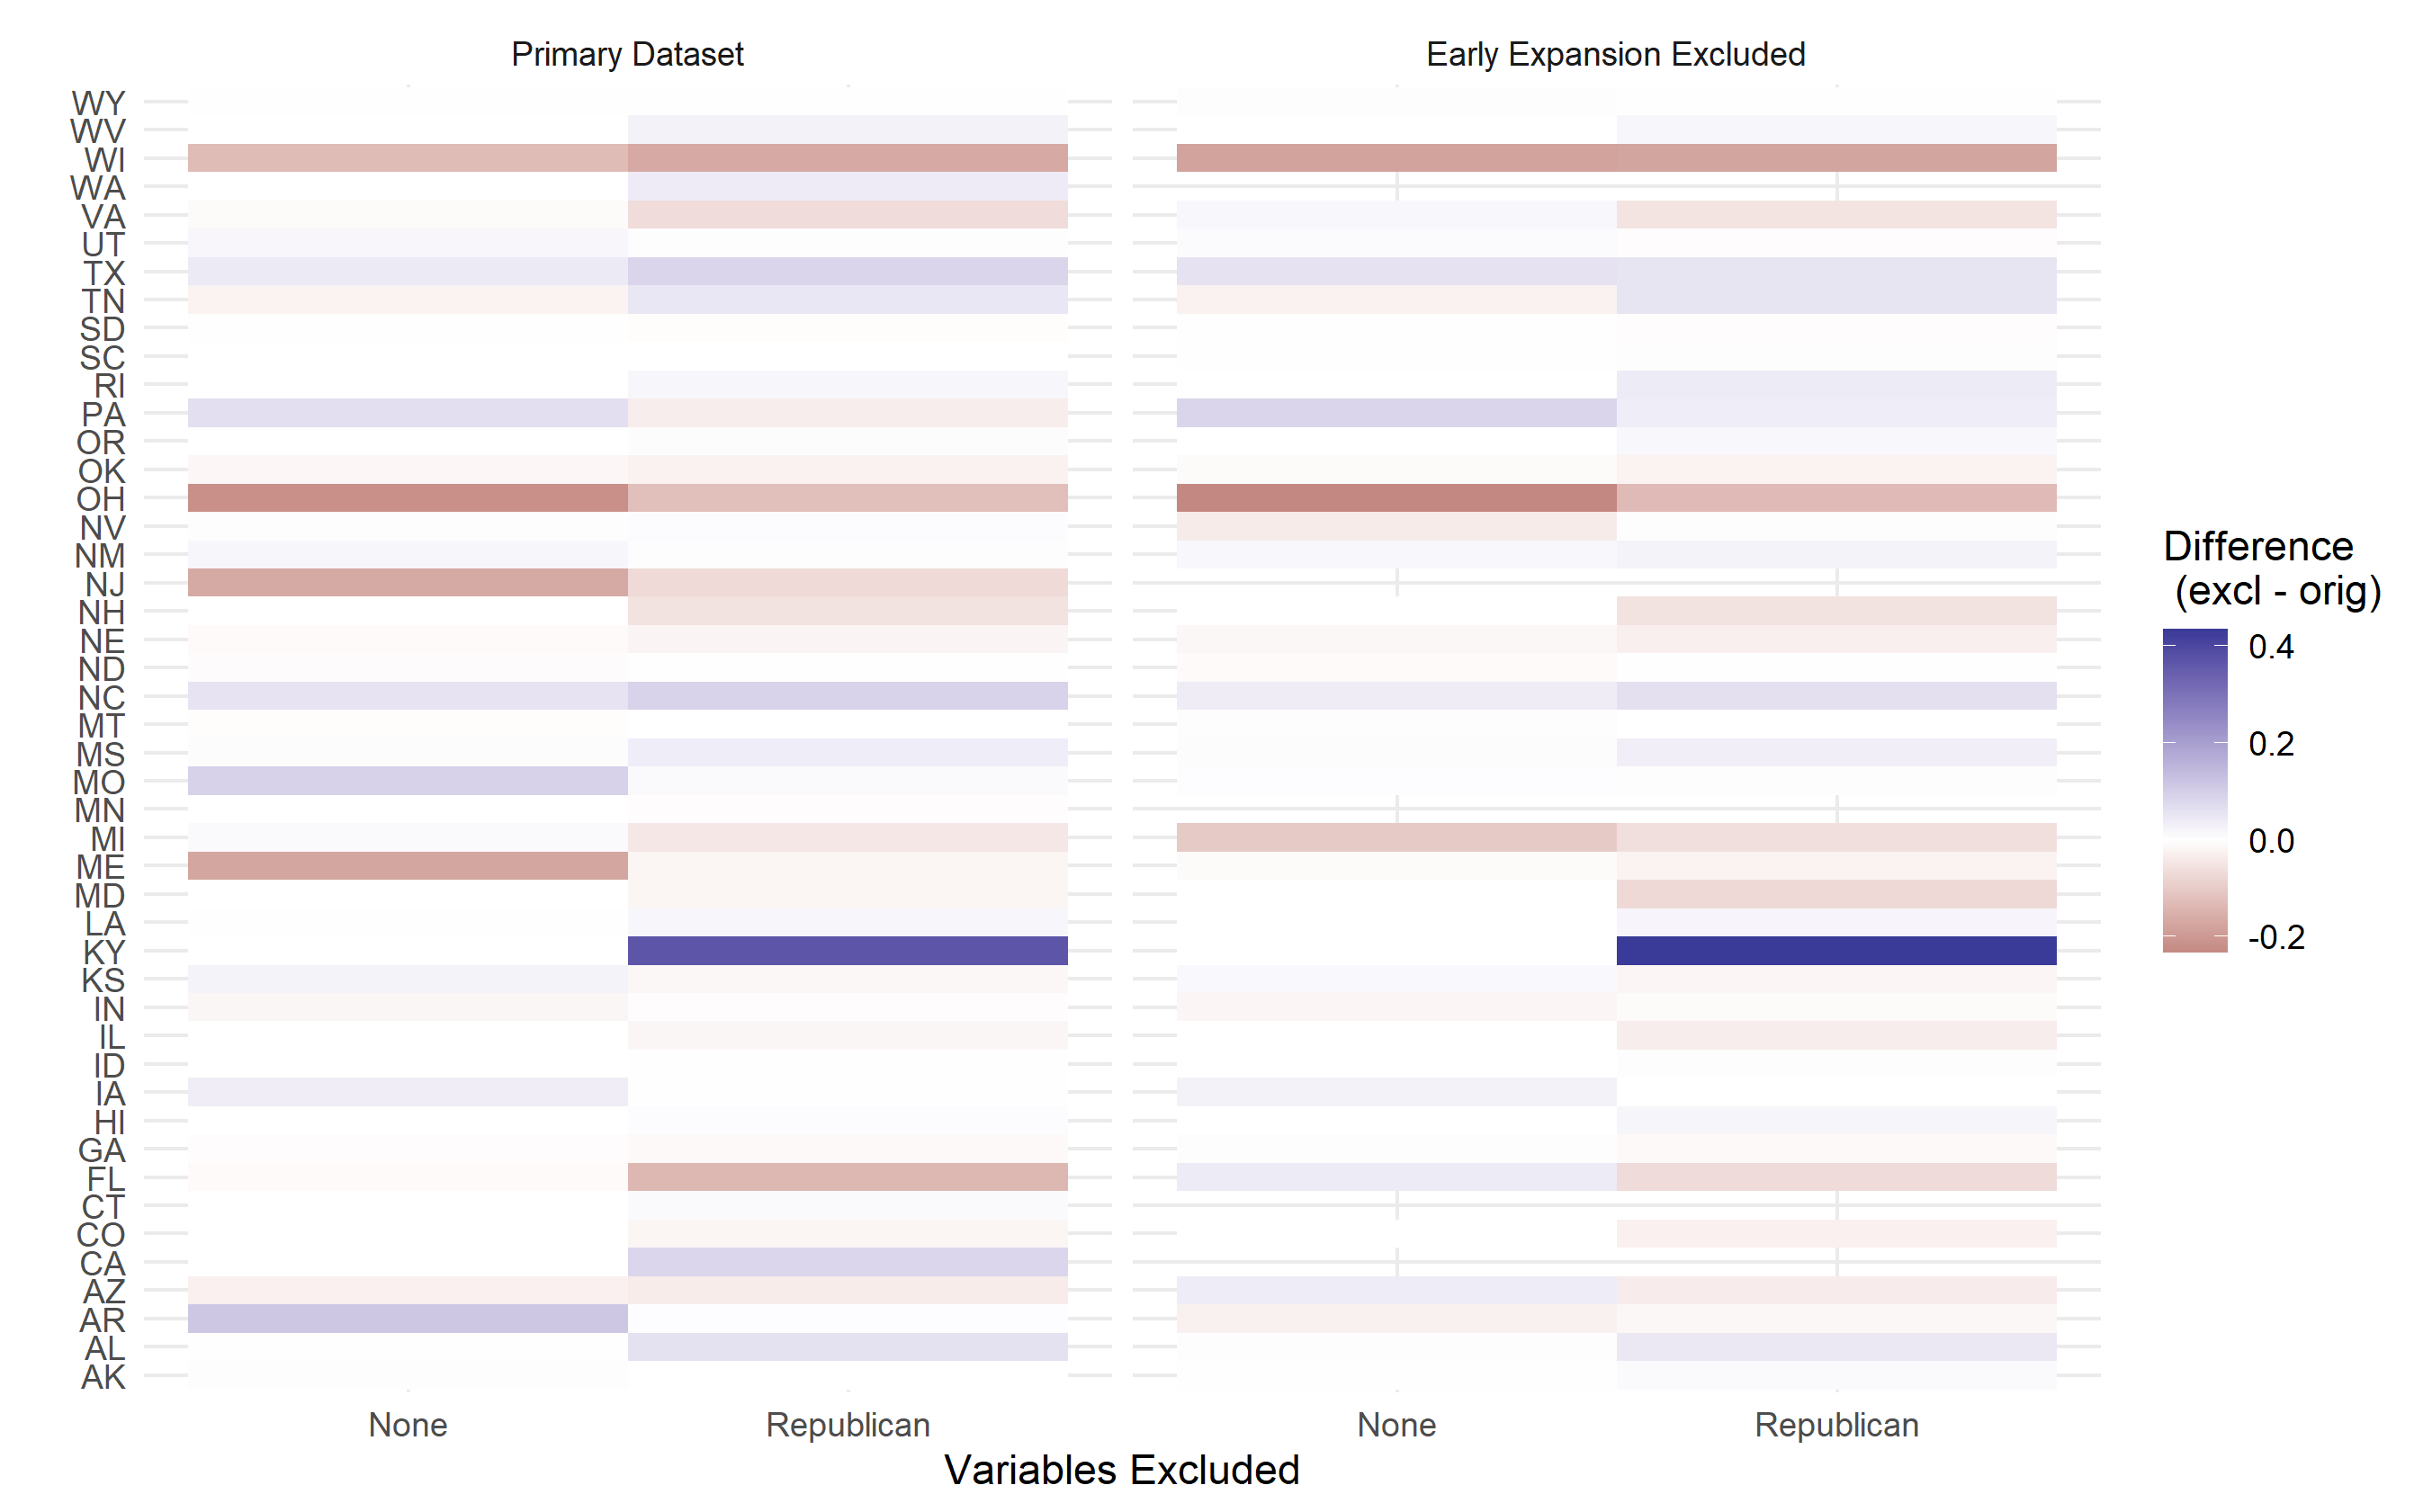
\includegraphics[scale=0.6]{01_Plots/oate-loo-state-cov-group-heatmap-states.png}
    \caption{OATE estimates, leave-one-out-states analysis}
    \label{fig:oateheatmap}
\end{center}
\end{figure}

\subsection{Appendix F: Miscellaneous Program Details}

We implement Stable Balancing Weights using a modification of Noah Griefer's ``optweight'' package available in R. The modifications are available on ``github.com/mrubinst757'', but are not documented. We use this program to generate weights that balance the means of the following covariates in the treated group to the control group within an error tolerance, $\delta$. When estimating the weights on different subsets of the data, $\delta^\star$ is not guaranteed to converge. We therefore modify the program so that if it does not converge, it relaxes some of the constraints until convergence. The program is available on github.com/mrubinst757/Medicaid-Expansion-Project/03\_RPrograms/03\_Analysis/02\_model-estimation.R and all R programs used to complete this analysis are available in the parent directory.

\end{document}






